% !TEX program = xelatex
% 酒店预订管理系统 设计与建模报告 —— 软件工程实验二
\documentclass[UTF8,a4paper,zihao=-4,fntsize=12pt]{ctexart}

\usepackage{geometry}
\geometry{top=2.5cm,bottom=2.3cm,left=2.5cm,right=2.5cm,headsep=6mm,footskip=9mm}
\usepackage{amsmath}
\usepackage{graphicx}
\usepackage{booktabs}
\usepackage{tabularx}
\usepackage{xltabular}
\usepackage{array}
\usepackage{enumitem}
\usepackage{fancyhdr}
\usepackage{caption}
\usepackage{subcaption}
\usepackage{capt-of}
\usepackage{needspace}
\usepackage{float}
\usepackage{placeins}
% 尽量让图与正文同页，减少整页只有一张图的空档
\renewcommand{\textfraction}{0.06}
\renewcommand{\topfraction}{0.92}
\renewcommand{\bottomfraction}{0.80}
\renewcommand{\floatpagefraction}{0.86}
\setcounter{topnumber}{3}
\setcounter{bottomnumber}{2}
\setcounter{totalnumber}{4}
\usepackage[hidelinks]{hyperref}

% ---------- 字体与排版 ----------
\linespread{1.35}
\setlength{\headheight}{14pt}
\setlength{\emergencystretch}{2em}
% 不留单行孤行（段首/段末各至少两行）
\widowpenalty=10000
\clubpenalty=10000
\setlength{\parskip}{0.35em}
\setlength{\parindent}{2em}
\raggedbottom
\setlist{nosep,leftmargin=3em,itemsep=2pt,topsep=3pt}

\ctexset{
  section = {
    name   = {,},
    number = \arabic{section},
    format = \heiti\zihao{3}\raggedright,
    aftername = \hspace{0.55em},
    beforeskip = 1.1em plus 0.2em minus 0.1em,
    afterskip  = 0.6em plus 0.1em minus 0.1em,
  },
  subsection = {
    name   = {,},
    number = \arabic{section}.\arabic{subsection},
    format = \heiti\zihao{4}\raggedright,
    aftername = \hspace{0.5em},
    beforeskip = 0.9em plus 0.15em minus 0.1em,
    afterskip  = 0.45em plus 0.1em minus 0.1em,
  },
  subsubsection = {
    name   = {,},
    number = \arabic{section}.\arabic{subsection}.\arabic{subsubsection},
    format = \heiti\zihao{-4}\raggedright,
    aftername = \hspace{0.4em},
    beforeskip = 0.7em plus 0.1em minus 0.1em,
    afterskip  = 0.35em plus 0.1em minus 0.1em,
  },
}

% ---------- 页眉页脚 ----------
\pagestyle{fancy}
\fancyhf{}
\fancyhead[C]{\zihao{5}\songti 软件工程实验二\quad 酒店预订管理系统设计与建模报告}
\fancyfoot[C]{\zihao{5}—\ \thepage\ —}
\renewcommand{\headrulewidth}{0.4pt}
\renewcommand{\footrulewidth}{0pt}
\fancypagestyle{plain}{%
  \fancyhf{}%
  \fancyfoot[C]{\zihao{5}—\ \thepage\ —}%
  \renewcommand{\headrulewidth}{0pt}%
}

% ---------- 图表 ----------
\renewcommand{\arraystretch}{1.15}
\renewcommand{\tablename}{表}
\renewcommand{\figurename}{图}
\captionsetup[table]{font=small,labelsep=quad,position=top,skip=5pt}
\captionsetup[figure]{font=small,labelsep=quad,position=bottom,skip=6pt}
\newcommand{\tabfont}{\zihao{5}}
% 窄列不要两端对齐，否则中文字距会被拉开成「字 距 稀 疏」
\newcolumntype{L}[1]{>{\raggedright\arraybackslash}p{#1}}

\hypersetup{
  pdftitle  = {酒店预订管理系统 设计与建模报告},
  pdfauthor = {曹继贤},
  pdfsubject= {软件工程实验二 · 软件设计与建模},
  pdfkeywords = {软件设计; UML; 架构设计; 数据库设计; UI 设计; 酒店预订}
}

\begin{document}

% ==================== 封面 ====================
\thispagestyle{empty}
\null\vfill
\begin{center}
{\zihao{3} 软件工程实验二}\\[2.2em]
{\heiti\zihao{1} 软件设计与建模报告}\\[1.4em]
\rule{0.62\textwidth}{0.8pt}\\[1.4em]
{\zihao{4} 酒店预订管理系统}\\[0.5em]
{\zihao{5} （小型单体酒店，承接实验一）}\\[3.2em]

{\zihao{4}
\renewcommand{\arraystretch}{1.6}
\begin{tabular}{r@{\hspace{1em}}l}
学\qquad 号 & 241220031 \\
姓\qquad 名 & 曹继贤 \\
指导教师 & 王\quad 豫 \\
实验日期 & 2026 年 11 月 7 日 \\
\end{tabular}}
\end{center}
\vfill
\newpage

% ---------- 目录 ----------
{\renewcommand{\contentsname}{目\quad 录}
\tableofcontents}
\newpage

% ==================== 一、项目与设计目标 ====================
\section{项目与设计目标}

\subsection{项目选择与承接关系}

本项目是实验一「需求分析」所选的第 \textcircled{4} 个题目——\textbf{小型酒店预订管理系统}的延续。实验一交付的是需求规格说明：四类角色（顾客、前台、店长、平台地区负责人）、两台状态机（订单六态、房间六态）、按「房型 $\times$ 日期」逐晚记录的库存模型、以及并发抢房、改价与下单互斥、价格快照等跨模块约束，共 36 条需求（其中已确认 34 条，REQ-035、REQ-036 仍标「待确认」）。

实验二的定位不同：\textbf{不写任何业务代码}，只把需求翻译成可以照着实现的设计。因此本报告自始至终遵守一条原则——\textbf{凡是能落到表结构、接口签名、状态转换表上的，就写实；凡是只能停留在口头描述的，就当成没设计}。报告里出现的每一个类、每一张表、每一个界面状态，都能回答「它对应哪条需求」和「实验三照着它能不能写出来」。

\subsection{设计目标}

\begin{enumerate}[leftmargin=3.2em]
  \item \textbf{不超卖}。同一房型同一晚最后一份库存，被 100 个请求同时抢，只能卖出 1 间；多晚订单中任一晚不足则整单失败，不留半截占用。
  \item \textbf{状态一致}。订单与房间各有一台状态机，非法转换一律拒绝而不是「尽力修正」；支付、取消、超时、未到店四个入口改的是同一行数据，且都带前置状态条件，谁先改成谁生效。
  \item \textbf{关键操作可追溯}。改价、开单、入住、取消、审批、删除，每一次写入都留操作人、时间、变更前后值；日志不提供修改与删除入口。
  \item \textbf{每个模块都有界面}。这是实验二的交付约束，也是本设计在模块划分阶段实际调整过划分的依据（见第七章 U-01）。
\end{enumerate}

\subsection{设计范围}

\begin{table}[H]
\centering
\caption{本次设计覆盖的内容与深度}
\tabfont
\begin{tabularx}{\textwidth}{@{}L{3.0cm}L{3.6cm}X@{}}
\toprule
设计项 & 产物 & 深度 \\
\midrule
软件的主要功能 & 第 2 章 + 表 \ref{tab:trace} & 36 条需求逐条映射到模块，标明跨模块与不覆盖的需求 \\
架构设计 & 第 3 章 + 包图、组件图、部署图 & 分层依赖规则、模块边界、依赖方向、部署形态写死 \\
数据存储设计 & 第 4 章 + 12 张表 & 字段、主键、唯一约束、索引；幂等与库存的约束落在具体列上 \\
行为建模 & 第 5 章 + 用例图、状态图、活动图 & 状态转换表穷举，非法转换给出处理方式 \\
交互建模 & 第 5 章 + 4 张时序图 & 抢房、支付回调、改价互斥、超时释放与对账 \\
UI 设计 & 第 6 章 + 16 屏界面 & 四端各屏的元素、状态与对应需求 \\
\bottomrule
\end{tabularx}
\end{table}

\subsection{明确不做的部分}

实验一已把会员、积分、优惠券、OTA 对接、在线开票划到范围之外（REQ-019），本设计同样不涉及。此外还有三处设计层面主动放弃的能力，写在这里以免读者以为漏了：

\begin{itemize}
  \item \textbf{不做微服务拆分}。本系统日均订单在百量级、门店十余间房，拆成多个服务只会把「扣库存 + 落单」这一个事务拆成两段，破坏不超卖的前提。模块边界按领域切，但部署为一个应用进程，见 3.5 决策一。
  \item \textbf{不做多活与异地容灾}。REQ-017 只要求营业时间可用性 99.5\%、故障 2 小时内恢复，主从 + 备份 + binlog 回放已经足够，多活会引入跨地域写冲突，与「库存只在一处串行扣减」直接矛盾。
  \item \textbf{不做动态定价}。REQ-023 明确「房价不与剩余房间数量挂钩」，因此系统里没有收益管理算法，价格是人定的，系统只负责守住平台下发的区间。
\end{itemize}

\subsection{统一的数据基准}

报告里 16 张 UML 图和 16 屏界面用的是同一套数据，读者可以拿界面上的数字去反查类图与表结构。基准如下（快照时刻 \textbf{2026-10-31 周六 13:47}）：

\begin{itemize}
  \item \textbf{门店}：湖滨银泰酒店，杭州西湖区，5 星，评分 4.6。
  \item \textbf{房型与楼层}：豪华双床房 24 间（1F、2F、6F），高级大床房 16 间（4F、5F），行政套房 8 间（3F），合计 48 间。
  \item \textbf{当日房态}（48 间）：在住 33、需打扫 7、已预定 3、维修中 2（408 水管、608 空调）、空闲 2、已退房 1，出租率 33/48 = 68.8\%。
  \item \textbf{当日价格}：高级大床房 ¥428/晚，豪华双床房 ¥498/晚，行政套房 ¥888/晚。
  \item \textbf{当日库存}（高级大床房）：总房量 16 − 线下保留 8 − 维修占用 1 = 线上可售上限 7，线上已售 3，剩余 4；次日 11-01 维修已结束，上限 8、已售 7、剩余 1，故「10-31 至 11-02 两晚」的可订量为 $\min(4,1)=1$ 间。
  \item \textbf{片区}：6 家门店、296 间房，当日营收 ¥113,721，加权出租率 72.7\%，平均房价（ADR）¥528.7。
\end{itemize}

\begin{quote}
\zihao{5}这套数字不是随手编的。它被三处交叉校验过：48 间的六种房态必须相加等于 48；48 间的价格 $\times$ 出租率必须能解释当日营收；片区 6 店的出租率按房量加权必须等于 72.7\%。界面上的每个数字改动都要过这三道校验，否则就是设计里出现了两套事实。
\end{quote}

% ==================== 二、软件的主要功能 ====================
\section{软件的主要功能}

\subsection{四类角色与各自的使用场景}

系统只有四类角色，且每类角色只在一端活动——这是 REQ-001「最小权限」在界面层面的直接体现：不同角色看到的不是同一套菜单的裁剪版，而是四套各自独立的前端。

\begin{table}[H]
\centering
\caption{角色、使用端与核心场景}
\tabfont
\begin{tabularx}{\textwidth}{@{}L{2.6cm}L{2.8cm}X@{}}
\toprule
角色 & 使用端 & 核心场景 \\
\midrule
顾客 & 手机 H5 & 搜房 $\rightarrow$ 看房型与实时余量 $\rightarrow$ 下单 $\rightarrow$ 15 分钟内支付 $\rightarrow$ 到店入住 $\rightarrow$ 退房后评价；入住日 18:00 前可自助取消 \\
前台 & 桌面工作台 & 看房态看板与今日待办 $\rightarrow$ 排房 $\rightarrow$ 3 步内办完入住 $\rightarrow$ 退房与派打扫 $\rightarrow$ 线下开单 $\rightarrow$ 18:00 后替顾客提取消申请 \\
店长 & 桌面后台 & 按日历定房价与线下保留额度 $\rightarrow$ 审批改价 / 取消 / 超限开单 / 维修派单 $\rightarrow$ 排班 $\rightarrow$ 看评价与绩效；对房态\textbf{只读} \\
平台地区负责人 & 桌面后台 & 向门店下发价格区间 $\rightarrow$ 审核跨店绩效 $\rightarrow$ 选派与调动店长 $\rightarrow$ 审批删除原始数据申请；\textbf{不得}代门店办理入住或改房态 \\
\bottomrule
\end{tabularx}
\end{table}

\subsection{九个业务模块与一个支撑模块}

模块按\textbf{业务能力}切分，不按角色切分：同一个模块的接口会同时被两端调用（例如「库存」既被顾客下单扣减，也被前台线下开单扣减、被店长改上限）。这样切的好处是一个业务概念只有一处实现，代价是模块数量与角色数量不对应，需要靠权限模块在入口处拦截。

\begin{table}[H]
\centering
\caption{模块与主要功能}
\tabfont
\begin{tabularx}{\textwidth}{@{}L{2.9cm}X@{}}
\toprule
模块 & 主要功能 \\
\midrule
M1 账号与权限 & 用户与角色维护；登录认证与会话签发；每个请求校验「角色 + 数据范围」；员工账号由上级分配；店长调动时权限实时回收 \\
M2 门店与房源 & 门店档案与营业状态；房型档案与上下架；房间档案（房号、楼层、房型归属、当前状态、预计修复日期）；对外提供房间总数与维修间数 \\
M3 定价 & 按「房型 $\times$ 日期」维护日价与价格来源；平台价格区间的接收与校验；改价申请与审批；为下单提供带锁取价 \\
M4 库存 & 按「房型 $\times$ 日期」逐晚维护上限、线上已售、线下保留、线下已售；下单条件扣减、取消与超时释放；按公式重算线上可售上限 \\
M5 预订与订单 & 订单状态机；下单（建单 + 扣库存同事务）；改期改房型；取消判定与退款发起；22:00 未到店与次日 12:00 逾期处理；订单查询 \\
M6 支付与退款 & 创建支付单；回调验签、按支付单号判重；原路退款；发布「支付成功」事件；每日对账与补单 \\
M7 房态与工单 & 房间状态机；空闲房间查询与排房占房；办理入住与退房；生成打扫与维修工单；工单执行与关闭 \\
M8 评价与绩效 & 已退房订单的一次性评价（1--5 星 + 文字）；门店与店长绩效汇总；跨店绩效供平台审核；排班与打卡 \\
M9 审计与数据保留 & 操作日志写入与分角色查询；3 年保留策略；半年绩效归档；删除原始数据的审批与执行 \\
M10 通知 & 订阅订单、支付、工单事件，按模板发短信与站内消息；失败重试与降级；失败不触发订单回滚 \\
\bottomrule
\end{tabularx}
\end{table}

其中 M1 与 M9 是\textbf{横切模块}——每一个业务模块都要校验权限、都要写审计日志，因此它们在组件图上不画十根箭头，而是合并成一根「公共支撑」箭头（见 3.3 节）。

\subsection{需求到模块的追溯矩阵}

下表把实验一的 36 条需求逐条映射到模块。功能需求 29 条中 28 条落到具体模块；非功能需求与范围约束横切全系统，在架构设计一节展开；两条待确认需求明确标注为不覆盖。

{\tabfont
\begin{xltabular}{\textwidth}{@{}p{1.55cm}p{4.15cm}p{3.5cm}X@{}}
\caption{REQ—模块追溯矩阵}\label{tab:trace}\\
\toprule
编号 & 需求名称 & 主要模块 & 落点说明 \\
\midrule
\endfirsthead
\toprule
编号 & 需求名称 & 主要模块 & 落点说明 \\
\midrule
\endhead
\midrule
\multicolumn{4}{r}{\zihao{6}续下页}\\
\endfoot
\bottomrule
\endlastfoot
REQ-001 & 角色定义与最小权限 & M1 & 角色与数据范围在会话中签发，网关逐请求校验 \\
REQ-002 & 顾客查询与预订 & M2、M4、M5 & 房源提供可售房型，库存给出余量，订单落单 \\
REQ-003 & 退房与评价提交 & M7、M8 & 退房改订单与房态；评价限已退房且一次 \\
REQ-004 & 前台办理入住 & M7 & 排房 + 入住两动作，同事务改房间与订单 \\
REQ-005 & 房间状态机 & M7 & 六态转换表驱动，非法转换抛异常 \\
REQ-006 & 店长门店管理 & M2、M3、M4、M7 & 日价在 M3，保留与上限在 M4，营业状态在 M2，房态只读在 M7 \\
REQ-007 & 平台地区负责人管理 & M1、M3、M8 & 调动在 M1，区间下发在 M3，跨店汇总在 M8 \\
REQ-008 & 订单状态机 & M5 & 六态转换表驱动，每次变更记来源 \\
REQ-009 & 取消与退款 & M5、M6 & 取消规则在 M5，退款执行在 M6 \\
REQ-010 & 重复提交防护 & M5 & 请求号唯一索引，重放返回原订单号 \\
REQ-011 & 并发抢房 & M4 & 条件更新写进 WHERE 子句，影响 0 行即失败 \\
REQ-012 & 改价与下单隔离 & M3 & 「房型 $\times$ 日期」粒度的锁，只覆盖写价这一个小段 \\
REQ-013 & 库存与可售上限 & M4 & 每晚一行，多晚一次扣减、整单回滚 \\
REQ-014 & 操作日志 & M9 & 只增不改，按角色数据范围过滤查询 \\
REQ-015 & 性能 & 横切 & 见 3.5 决策七 \\
REQ-016 & 安全 & 横切 & 见 3.5 决策八 \\
REQ-017 & 可靠性与数据一致 & 横切 & 见 3.5 决策三、部署图 \\
REQ-018 & 易用性 & 横切 & 入住 3 步，见第 6 章 09 屏 \\
REQ-019 & 范围约束 & 约束 & 不进入本期设计 \\
REQ-020 & 支付超时释放 & M5、M6 & 状态条件更新 + 同事务释放 \\
REQ-021 & 取消截止与前台代取消 & M5 & 18:00 为界，之后转审批 \\
REQ-022 & 未到店标记与迟入住 & M5、M7 & 定时任务判状态，M7 只回答「今天入住了没有」 \\
REQ-023 & 价格快照与定价依据 & M3、M5 & 快照写在订单明细行上，改价不回写 \\
REQ-024 & 房号分配 & M7 & 排房占房记录，唯一约束防重复占用 \\
REQ-025 & 房态变更工单 & M7 & 工单是改房态的唯一入口 \\
REQ-026 & 员工信息可见范围 & M1 & 数据范围规则，店长限本店 \\
REQ-027 & 输入校验与错误提示 & 横切 & 服务端独立校验，见 3.4 节 \\
REQ-028 & 支付与订单一致性 & M6、M5 & 对账补单，库存不足则退款 \\
REQ-029 & 通知失败处理 & M10 & 独立失败队列，不参与订单事务 \\
REQ-030 & 数据保留与删除审批 & M9 & 3 年保留 + 审批后删除 \\
REQ-031 & 订单变更 & M3、M4、M5 & 差额调库存，按新价重算快照 \\
REQ-032 & 多房型多晚次组合 & M4、M5 & 一单多明细，明细粒度是「房型 $\times$ 日期」 \\
REQ-033 & 线上可售上限与线下保留 & M2、M4 & 总数与维修数来自 M2，上限公式在 M4 \\
REQ-034 & 维修中与可售上限联动 & M2、M4、M7 & 维修标记在 M2，逐日扣减在 M4，入口在 M7 \\
REQ-035 & 订单排房时限 & —— & 实验一待确认，本设计不覆盖 \\
REQ-036 & 账号注册与登录 & —— & 实验一待确认，本设计不覆盖 \\
\end{xltabular}
}

\subsection{一笔订单的完整链路}

把上表横过来看：一笔订单从产生到终结，会依次穿过 M2、M3、M4、M5、M6、M7、M8、M10 八个模块。这条链路上有四个「状态会分叉」的时刻，它们是后面所有图与表的重点：

\begin{enumerate}[leftmargin=3.2em]
  \item \textbf{下单}：先扣库存再建单，同一事务。扣库存是链路上唯一会失败的关键动作，放在最前，失败的请求尽早退出，不浪费订单号分配。
  \item \textbf{支付}：回调改状态与超时任务改状态改的是同一行，都带「状态 = 待支付」条件，谁先改成谁生效。
  \item \textbf{入住}：房间从空闲变已预定，订单从已确认变已入住，两个状态机在同一个操作里各走一步。
  \item \textbf{取消}：18:00 前立即生效，18:00 后转审批；未到店订单取消不退房费；重复提交只退一次。
\end{enumerate}

% ==================== 三、软件架构设计 ====================
\section{软件架构设计}

\subsection{为什么是「分层 + 领域模块化」}

实验一的需求里，真正难的从来不是「把界面做出来」，而是三件会互相打架的事：库存不能被两个人同时卖出、改价不能和下单撞在半个价格上、订单与房间两个状态机必须同步推进。这三件事的共同点是——\textbf{它们都要求某个最小粒度的东西只有一个权威副本}。库存的权威副本是「房型 $\times$ 日期」这一格，价格的权威副本也是这一格，订单状态的权威副本是订单表的 `status` 列。

由此推出架构的第一条约束：\textbf{任何可能被并发写入的业务概念，只能有一个存储点、一种写入口}。这条约束直接决定了系统长成「单体应用 + 一个 MySQL」，而不是微服务。

第二条约束来自角色：四个端面对的界面完全不同，但它们操作的是同一批业务对象。如果把「顾客端下单」和「前台线下开单」写成两套扣库存逻辑，两边迟早会对不上，超卖只是时间问题。因此表现层可以分裂成四套，\textbf{领域层必须合并成一套}。

两条约束合起来，就是本设计采用的架构风格：\textbf{按层分离部署形态，按领域划业务模块，模块之间单向依赖，事件解耦环}。

\subsection{分层与包结构}

图 \ref{fig:pkg} 是包图。四层从上到下依次是表现层、接入层、领域层、基础设施层，依赖方向严格向下，不允许反向。

\begin{figure}[htbp]
\centering
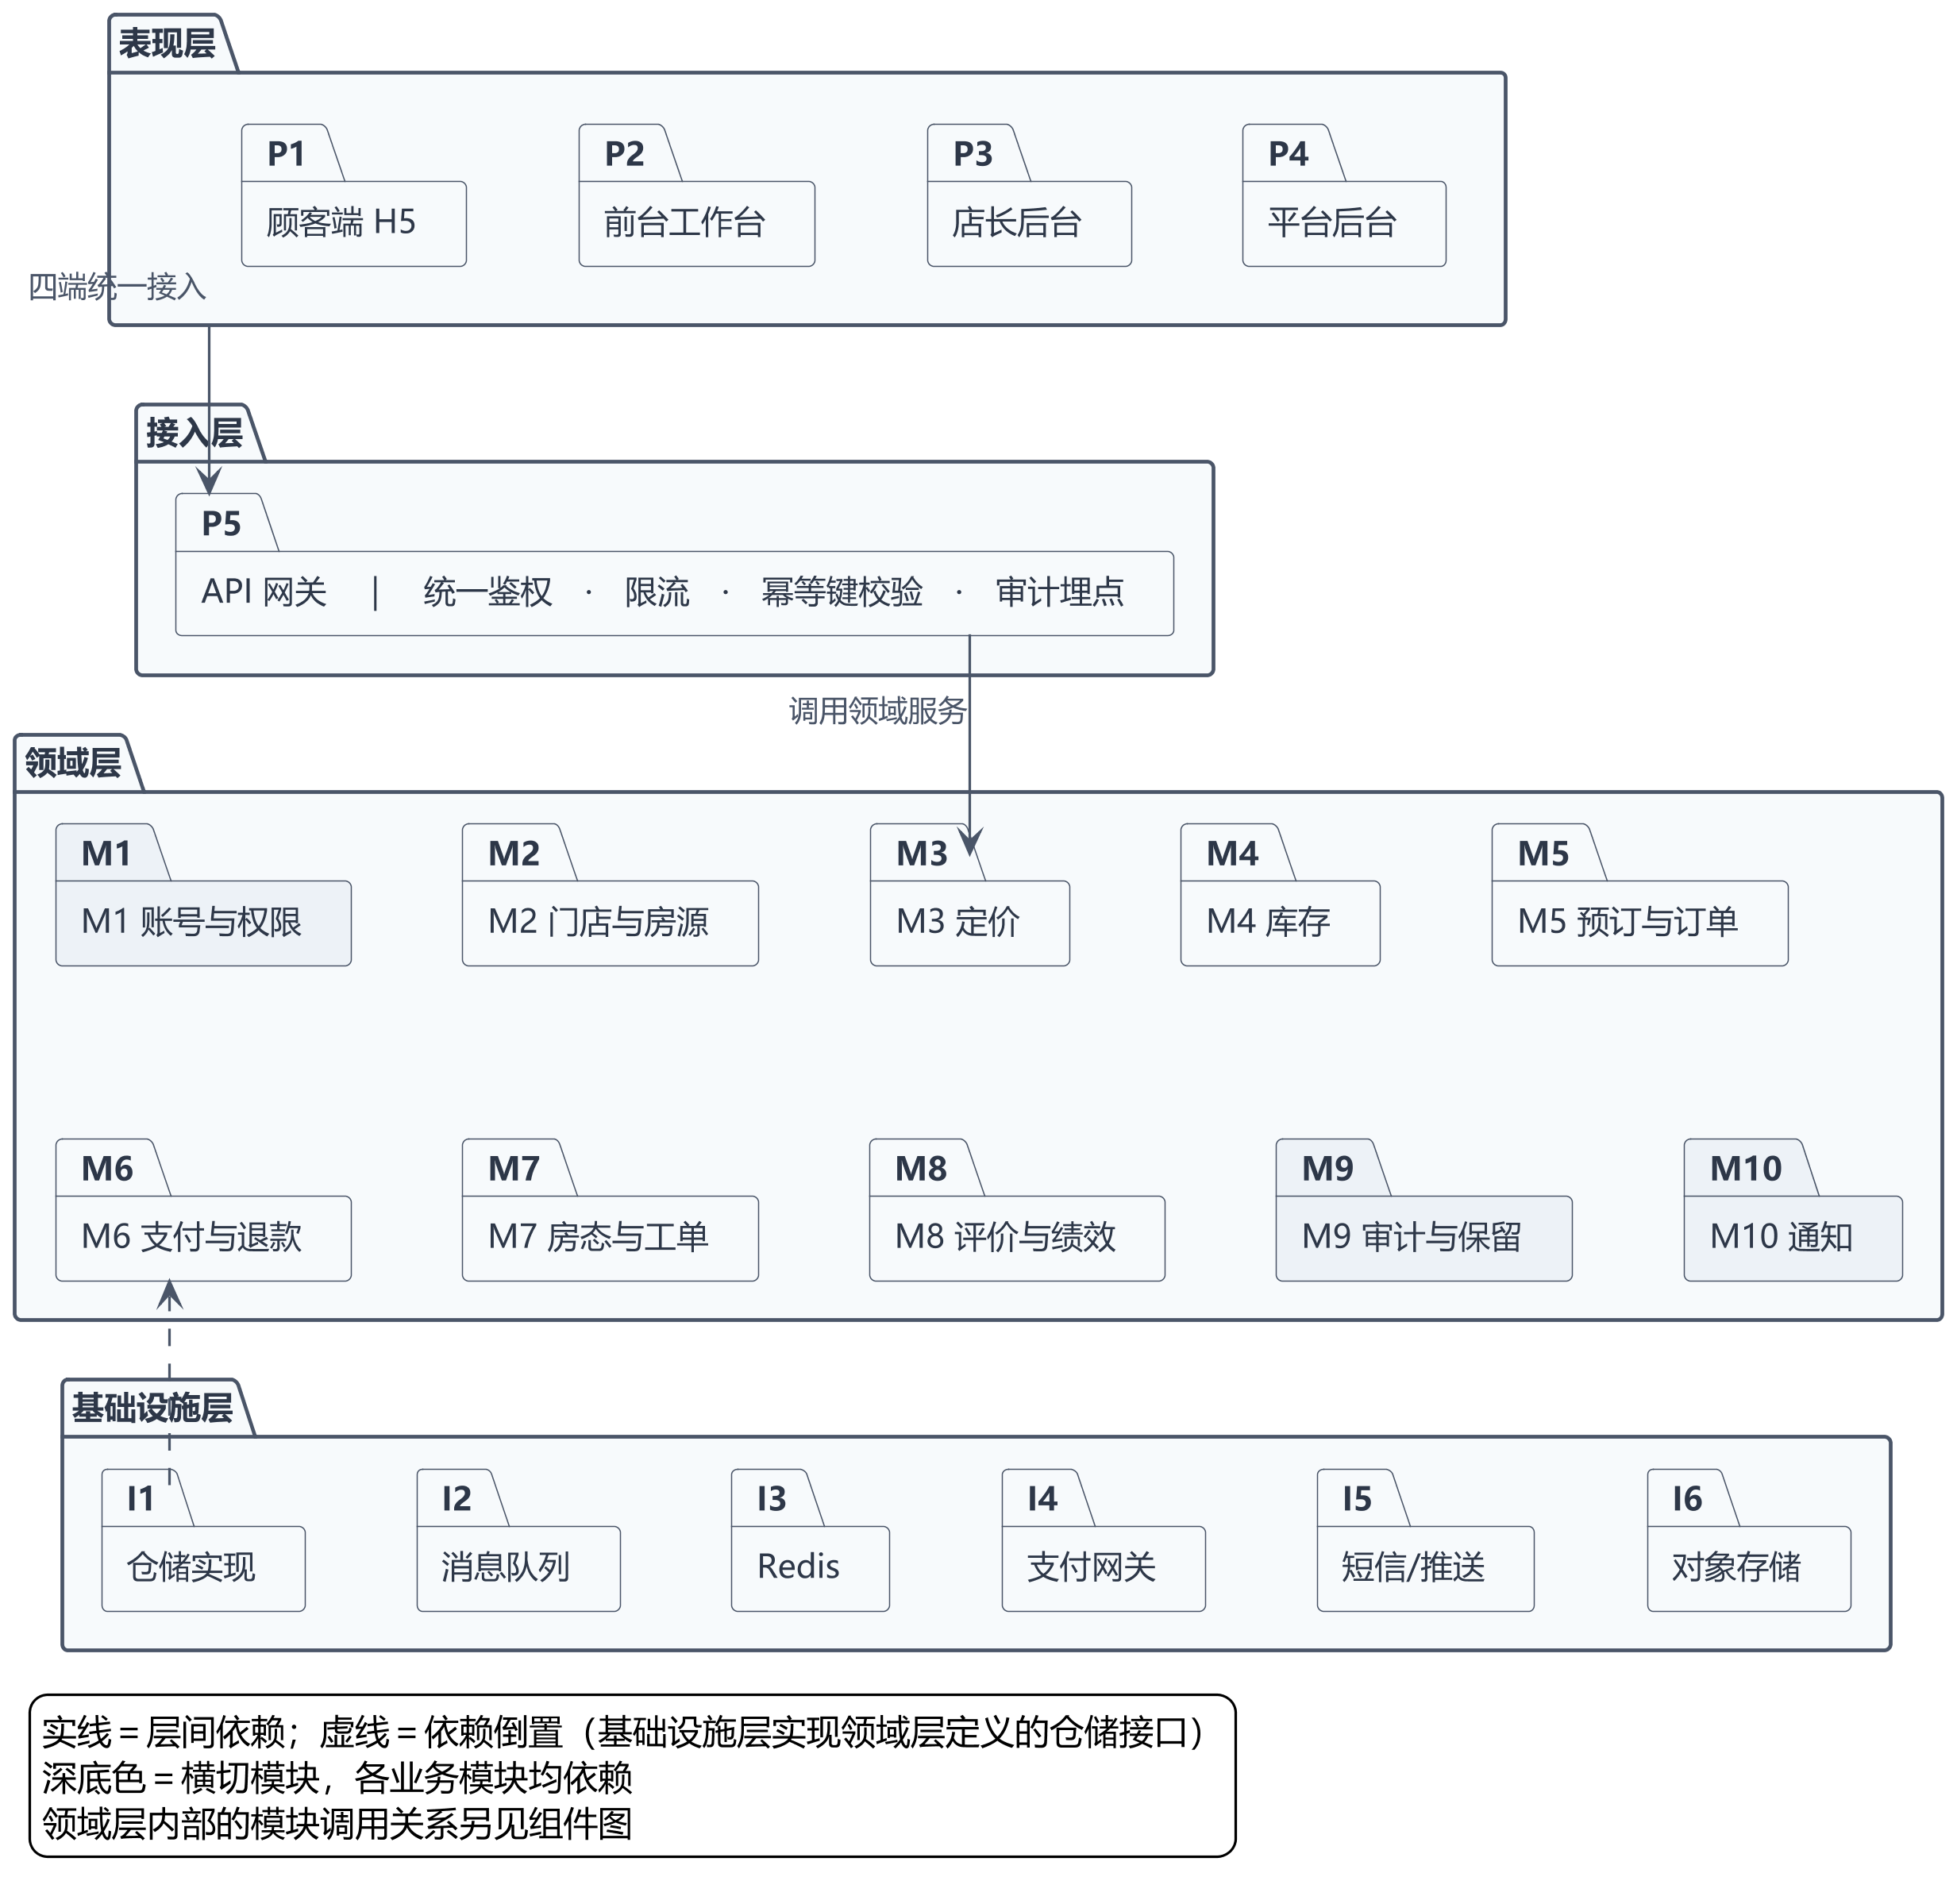
\includegraphics[width=0.96\textwidth]{../UML/UML包图.png}
\caption{UML 包图：四层结构与十个领域包}
\label{fig:pkg}
\end{figure}

四个层的职责与被禁止的动作：

\begin{itemize}
  \item \textbf{表现层}：四个独立前端，只做渲染与表单校验。不允许把业务规则写在前端——REQ-027 明确要求服务端独立校验，前端的校验只是体验，不是保障。
  \item \textbf{接入层}：API 网关，做鉴权、限流、幂等键校验、审计埋点。它是唯一知道「谁在调用」的地方，因此也是最省事的越权拦截点。
  \item \textbf{领域层}：十个模块，全部业务规则在这里。领域层\textbf{不认识} HTTP，也不认识具体数据库——它依赖的是仓储接口。
  \item \textbf{基础设施层}：仓储实现、消息队列、Redis、支付网关适配、短信适配、对象存储。它实现领域层定义的接口，箭头是\textbf{反向的虚线}（依赖倒置）：不是领域层去 new 一个 MySQL，而是基础设施层去实现它。
\end{itemize}

包图里有一条不太显眼但很关键的约束：\textbf{领域层内部没有跨越层的捷径}。例如 M5 想释放库存，必须走 M4 的接口，不能直接更新 `日库存` 表。这条约束看起来啰嗦，但它保证了「库存只有 M4 会改」——一旦允许绕过，REQ-011 的并发正确性就失去了推理基础。

\subsection{模块划分与依赖关系}

\subsubsection{组件图读法}

图 \ref{fig:comp} 是组件图。实线是调用依赖，虚线是事件订阅，方向即依赖方向。

\begin{figure}[htbp]
\centering
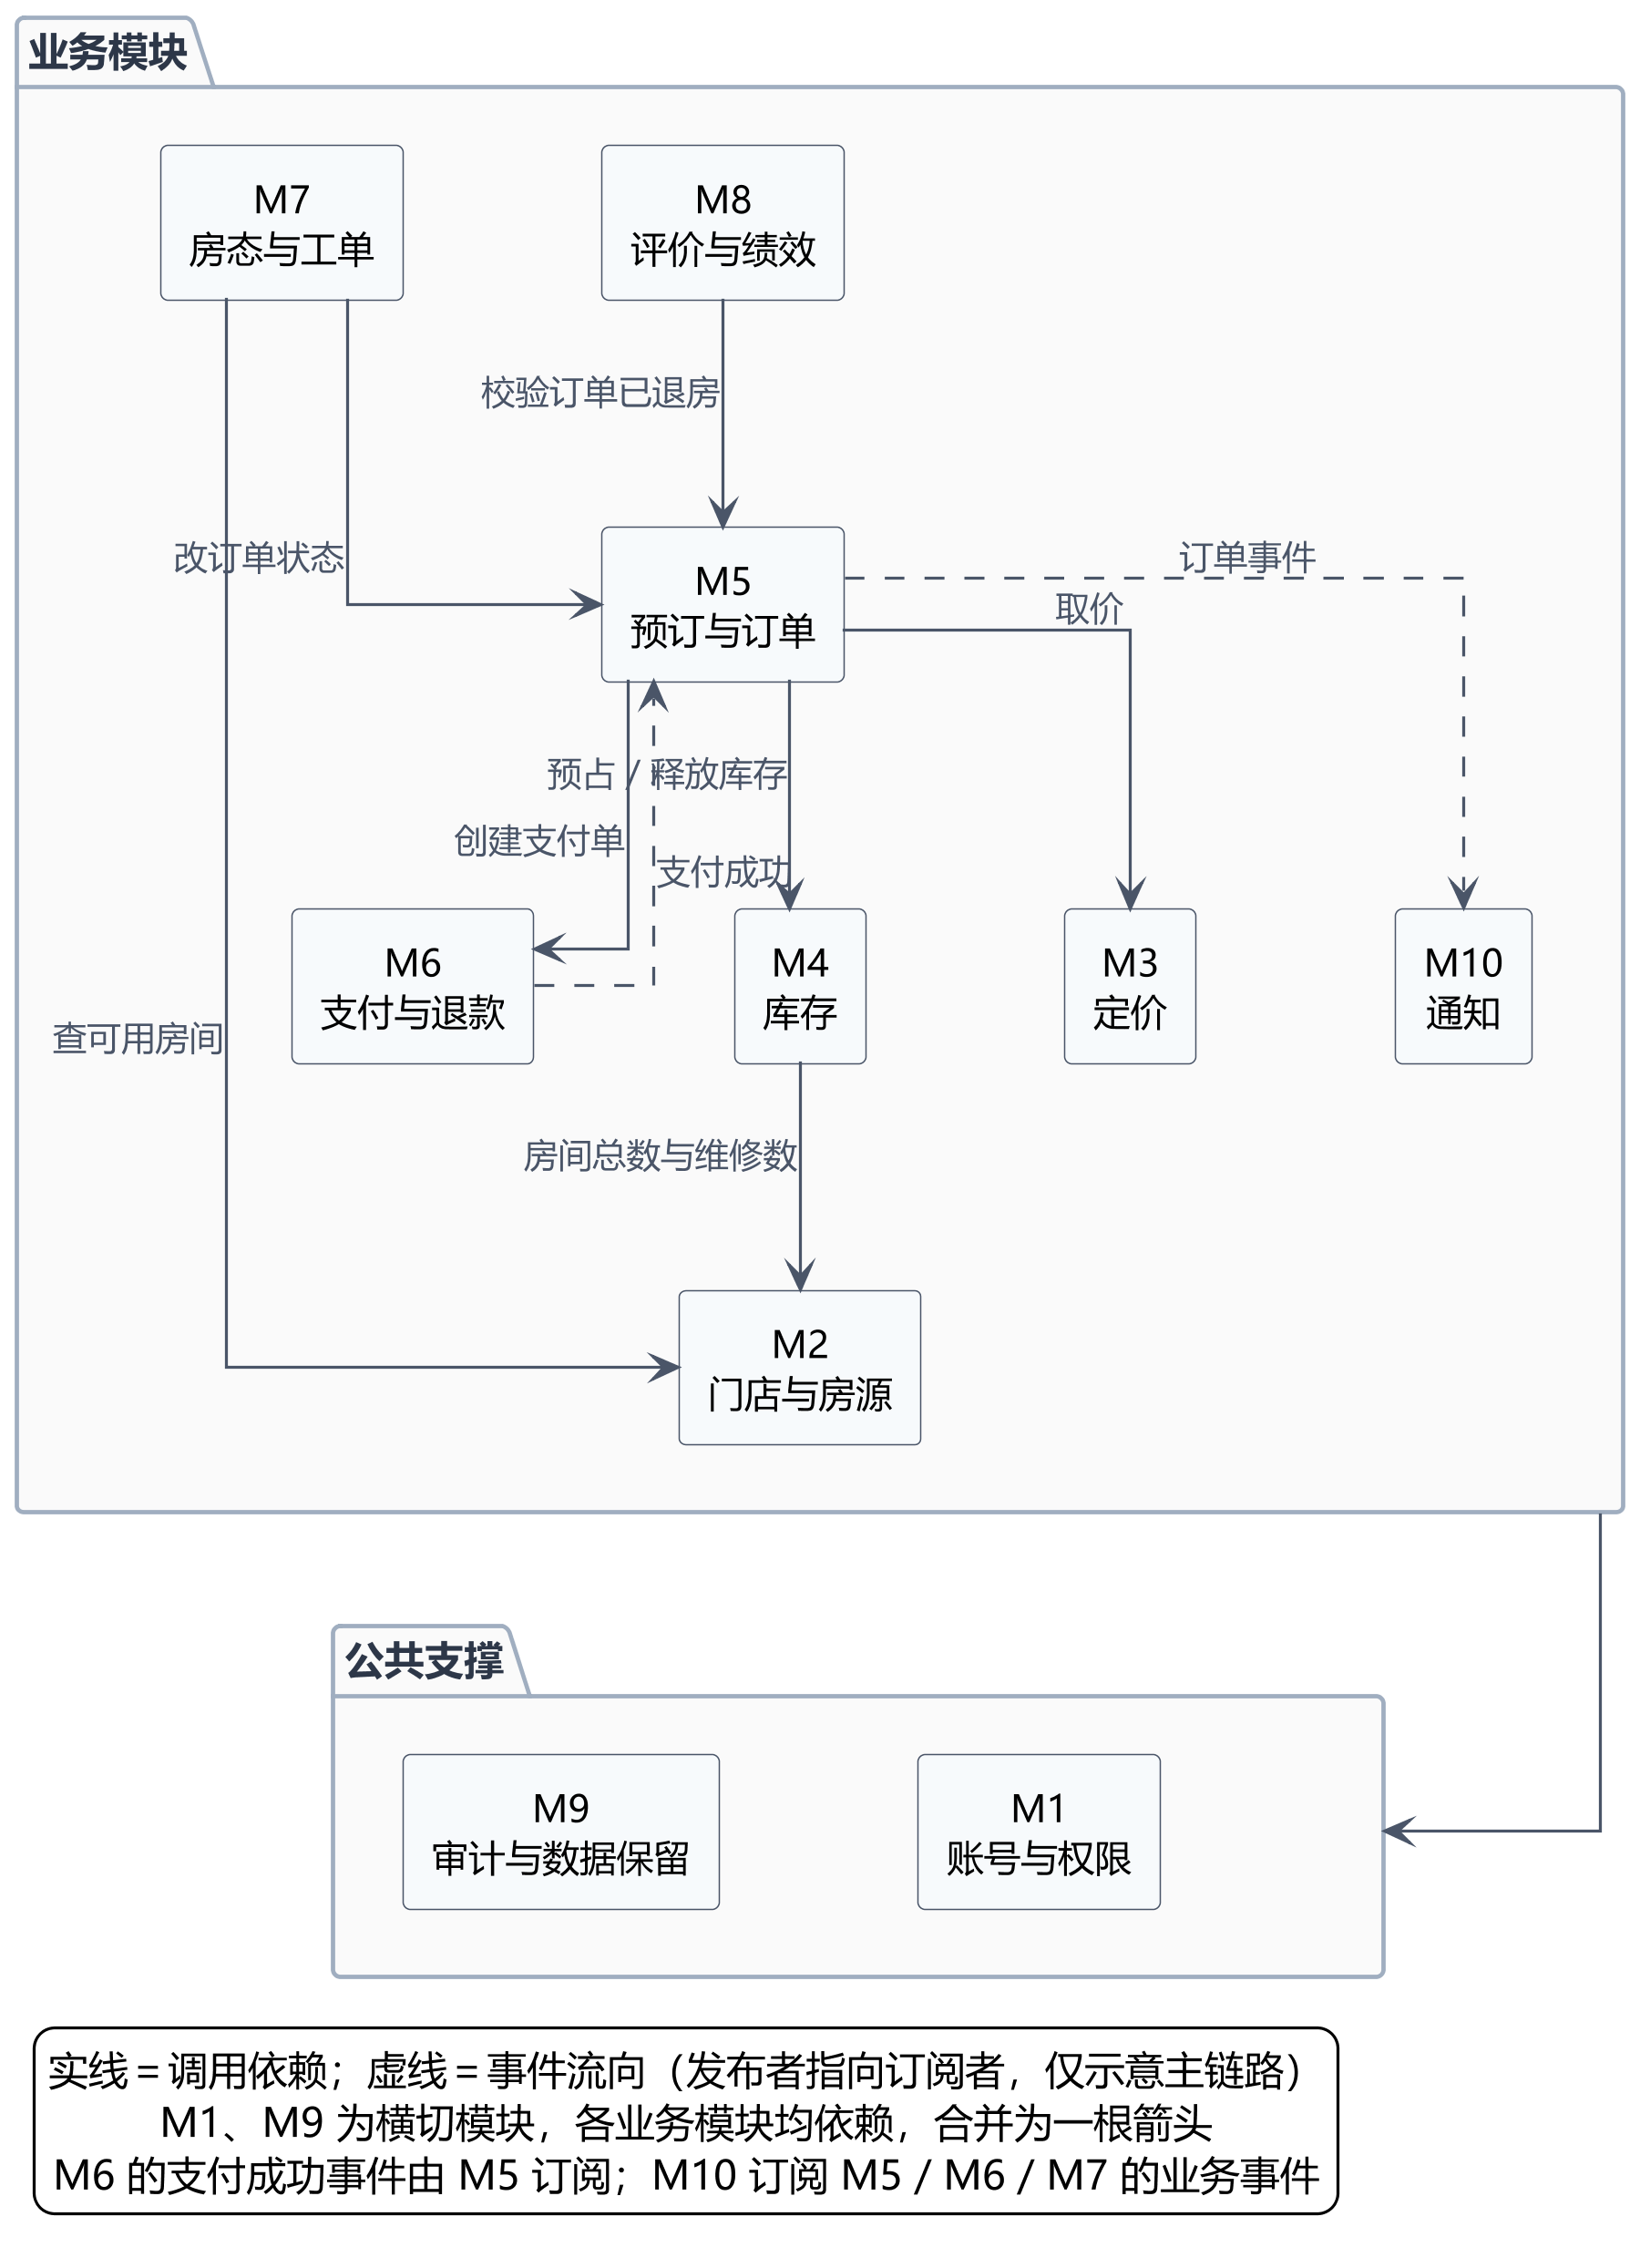
\includegraphics[width=0.68\textwidth]{../UML/UML组件图.png}
\caption{UML 组件图：十个模块的调用依赖与事件订阅}
\label{fig:comp}
\end{figure}

图上有\textbf{九条}依赖，逐条都有对应的业务事实：

\begin{table}[H]
\centering
\caption{组件图上的依赖及其依据}
\tabfont
\begin{tabularx}{\textwidth}{@{}L{2.5cm}L{1.8cm}X@{}}
\toprule
依赖 & 类型 & 为什么存在 \\
\midrule
M5 $\rightarrow$ M4 & 调用 & 下单预占、取消与超时释放库存（REQ-011、REQ-013） \\
M5 $\rightarrow$ M3 & 调用 & 下单取价并生成价格快照（REQ-023） \\
M5 $\rightarrow$ M6 & 调用 & 用户点「去支付」时创建支付单（不在下单时创建，见决策四） \\
M6 $\rightarrow$ M5 & 事件 & 支付成功后 M6 只发事件，M5 订阅后自行推进订单状态 \\
M4 $\rightarrow$ M2 & 调用 & 计算可售上限需要房间总数与维修间数（REQ-033、REQ-034） \\
M7 $\rightarrow$ M2 & 调用 & 排房时查询可用房间（REQ-024） \\
M7 $\rightarrow$ M5 & 调用 & 入住与退房要同步推进订单状态（REQ-004） \\
M8 $\rightarrow$ M5 & 调用 & 提交评价前校验订单已退房（REQ-003） \\
M5、M6、M7 $\rightarrow$ M10 & 事件 & 订单、支付、工单事件触发通知（REQ-029） \\
\bottomrule
\end{tabularx}
\end{table}

\subsubsection{三处边界约定的理由}

模块划分最容易被质疑的不是「切成了几块」，而是「某个职责为什么放在这块」。本设计有三处是讨论后才定的，都写在这里：

\textbf{一、维修标记放在 M2 的房间档案上，M7 只是改它的入口。} 库存要算可售上限，必须拿到「这间房在哪些日期维修」，而库存不能反过来依赖房态模块——那会让库存回算路径变成 M4 $\rightarrow$ M7 $\rightarrow$ M2 三段。把维修日期作为房间档案的一个字段，M4 只需要依赖 M2 一段。代价是 M7 改房态时写的是 M2 的表，看起来越界，但这是有意为之的取舍。

\textbf{二、排房归 M7，不归 M2。} M2 只管「这栋楼有几间房、几间在修」，是静态档案；「今天这间房被哪张订单占着」是动态事实，属于房态。若把排房交给 M2，M2 就要持有占房记录并维护唯一性，而它原本是无状态的档案模块。

\textbf{三、M10 只订阅事件，绝不反向调用业务模块。} 这条约束的意思是：事件载荷里必须带够渲染通知所需的字段（订单号、金额、顾客联系方式、时间），M10 不能回头查 M5 补全。不守住这条，实验三实现时一定会退化成「M10 调 M5 查订单」，于是通知模块一旦故障就会拖慢下单。

\subsubsection{横切模块的画法}

M1 账号与权限、M9 审计与数据保留被所有业务模块依赖。组件图上没有画十根箭头——那样图会被压成一张蜘蛛网，反而看不出业务模块之间的关系。折中的画法是把两者放进「公共支撑」带，各业务模块汇一根箭头指过去。

这里需要说明的是：\textbf{这个折中本身是违反「画全」原则的}，因为 M1、M9 在图上的连线不完整。做出这个选择的原因是作业要求「写明软件的模块划分」，一张看不出结构的完整图等于没画；而缺失的那部分信息在上表与本节文字里已经补齐。

\subsection{模块之间的交互}

组件图只说了「谁依赖谁」，没说「什么时候、按什么顺序」。这要靠时序图与活动图（图 \ref{fig:seq1}--\ref{fig:act2}，说明见 5.4 节）。这里先概括三处最关键的交互：

\subsubsection{下单与扣库存}

顾客提交订单时携带请求号，网关按请求号做幂等校验，M5 在同一事务内完成「条件扣减库存 + 插入待支付订单」。库存扣减写在 SQL 的 WHERE 子句里：

\begin{quote}
\zihao{5}\ttfamily
UPDATE inventory SET sold = sold + n\\
WHERE room\_type = ? AND stay\_date = ? AND sold + n <= online\_limit
\end{quote}

影响 0 行就是抢房失败，不需要「先查再改」。这不是性能优化，而是正确性要求：先查再改之间只要有间隙，100 并发下必然超卖（REQ-011、REQ-015）。

\subsubsection{支付回调与订单生效}

支付平台异步回调时，M6 依次做三件事：验签、按支付单号判重、按订单\textbf{此刻}的状态决定落点。状态是待支付就转已确认并保留库存；状态已被超时任务改成已取消，就不再恢复订单——库存可能已经被别人买走——而是发起原路退款。这条分支是 REQ-028「不得出现已扣款而无对应订单」的具体实现。

\subsubsection{改价与下单互斥}

店长改价与顾客下单在同一格「房型 $\times$ 日期」上互斥，锁的范围只覆盖「读旧价 $\rightarrow$ 写新价 $\rightarrow$ 提交」这一小段，毫秒级。等锁超过 300 ms 就返回重试提示，\textbf{不允许静默使用旧价}——静默用旧价等于把一次改价悄悄吞掉。

\subsection{部署形态}

\begin{figure}[htbp]
\centering
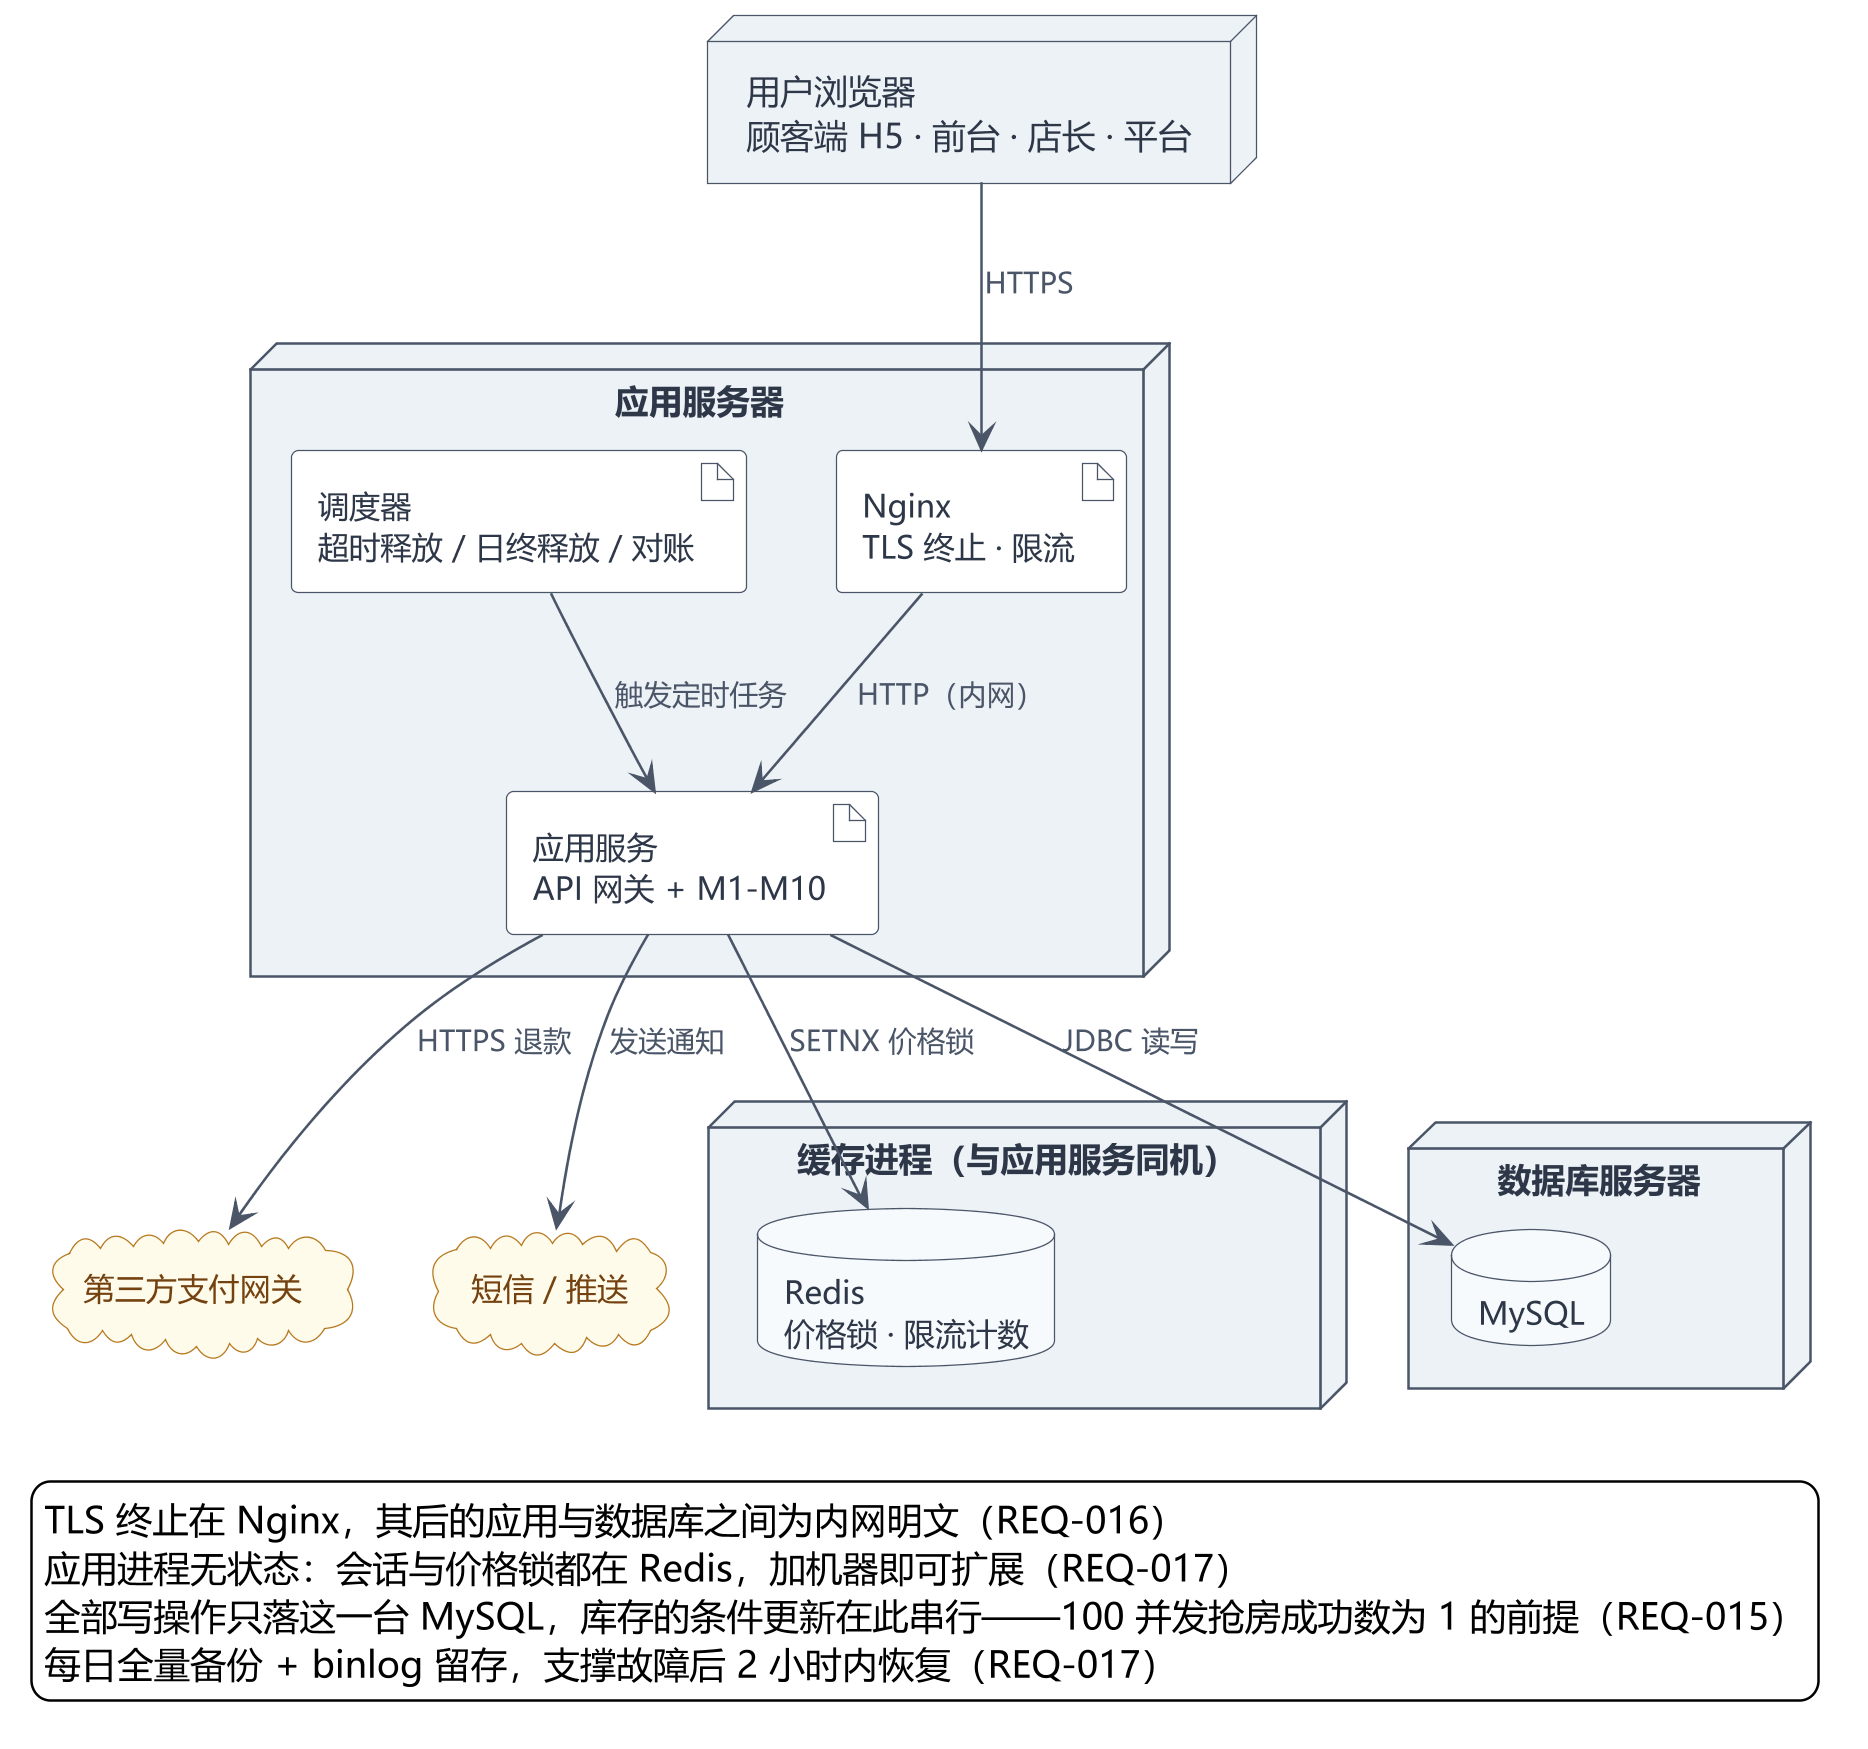
\includegraphics[width=0.92\textwidth]{../UML/UML部署图.png}
\caption{UML 部署图：应用、缓存、数据库与三类外部系统}
\label{fig:deploy}
\end{figure}

图 \ref{fig:deploy} 是部署图，四个要点：

\begin{itemize}
  \item \textbf{TLS 终止在 Nginx}，其后应用与数据库之间为内网明文。这不是省事，而是内网段本身不对外，再做一层 TLS 只会增加证书轮换成本（REQ-016 只要求「全站通过 HTTPS 传输」，指的是用户侧）。
  \item \textbf{应用进程无状态}：会话与价格锁都在 Redis，加机器即可扩展。这意味着可以横向加应用节点，但\textbf{不能}横向加数据库——库存的条件更新必须在同一台 MySQL 上串行，这是 100 并发抢房成功数为 1 的前提。
  \item \textbf{调度器与应用同机部署}，负责支付超时扫描、日终保留释放、每日对账。选同机是因为它只是一个定时触发循环，拆成独立进程反而要多一套部署与监控。
  \item \textbf{唯一写库}：去掉主从读写分离对写的影响，读请求可以走从库，写请求全部落主库。
\end{itemize}

\subsection{八条关键设计决策与代价}

架构设计最容易被问的问题是「为什么不那样做」。下面八条是本设计里争议最大、也最需要说清代价的取舍。

{\tabfont
\begin{xltabular}{\textwidth}{@{}p{0.5cm}p{3.3cm}X@{}}
\caption{关键设计决策与代价}\label{tab:decisions}\\
\toprule
\# & 决策 & 取舍与代价 \\
\midrule
\endfirsthead
\toprule
\# & 决策 & 取舍与代价 \\
\midrule
\endhead
\midrule
\multicolumn{3}{r}{\zihao{6}续下页}\\
\endfoot
\bottomrule
\endlastfoot
一 & 单体应用而非微服务 & 换来「扣库存 + 落单」是一个本地事务，不超卖可以只靠数据库保证。代价是模块只能靠代码边界约束，不能靠进程隔离；某个模块内存泄漏会拖垮全站。以本系统的量级（日均百单、十余间房），这个代价可以接受。 \\
二 & 库存记在「房型 $\times$ 日期」而非房间上 & 下单时顾客并不知道住哪间，REQ-024 也是「先占房型、入住前才排房」。代价是查询余量要按日期范围聚合，且排房时需要另一次「房间是否被占」的判定——这个判定落在 M7 的占房记录上。 \\
三 & 库存只信 MySQL 行锁，Redis 不承担计数 & 换来不存在「缓存与数据库双写不一致」这一类问题，REQ-017 的数据一致性有单点可依。代价是并发高峰时库存这一行会成为热点行，吞吐受限；本系统的峰值并发是 100 个请求抢 1 间房，MySQL 足够。 \\
四 & 支付单在「去支付」时创建，不在下单时创建 & 换来支付网关故障不波及下单——网关挂了，顾客仍能正常下单，只是暂时付不了款。代价是订单与支付单不是同时产生的，对账时可能出现「订单存在但无支付单」的正常中间态，判断差异时必须排除超时未支付这一种。 \\
五 & 订单与房间各一台状态机，转换表驱动 & 换来非法转换有唯一处理方式（抛异常并提示当前实际状态），而不是各处的 if-else 各写各的。代价是每次新增状态都要同时改三处：状态枚举、转换表、界面文案，漏一处就会在某个入口上崩。 \\
六 & 订单明细存价格快照 & 换来改价不影响历史订单（REQ-023），退款金额也有据可查。代价是订单表与价格表之间多一份冗余，出现「同一晚两个价格」时必须能解释清楚哪一个是快照、哪一个是当前价——界面上不展示当日价时不标「当前价」就是错的。 \\
七 & 查询走缓存，写一律落主库 & REQ-015 要求 50 并发下查询 2 秒内返回。房型与价格是读多写少，加一层本地缓存即可满足；写请求不缓存，避免为了刷新缓存引入一致性窗口。代价是改价后最多有一个缓存 TTL 的延迟，本设计把 TTL 设为 5 秒，并在改价成功后主动失效该房型当日的缓存条目。 \\
八 & 鉴权在网关一次做完，领域模块不重复鉴权 & 换来权限规则只有一处，改一次全站生效（REQ-016）。代价是领域模块被内部服务直接调用时没有防线，因此约定：领域模块的接口\textbf{只能}由网关或本进程内的上游模块调用，不对外开放端口。 \\
\end{xltabular}
}

% ==================== 四、数据库设计 ====================
\section{数据库设计}

\subsection{设计原则}

数据库表结构重点落实以下约束：

\begin{enumerate}[leftmargin=3.2em]
  \item 请求号唯一，防止重复创建订单（REQ-010）。
  \item 库存扣减采用条件更新，防止同一房型同一晚超卖（REQ-011）。
  \item 房间与晚次的组合唯一，防止重复排房（REQ-024）。
\end{enumerate}

字段类型采用以下约定：

\begin{itemize}
  \item 金额使用 \texttt{DECIMAL(10,2)}，供订单金额与支付金额比对。
  \item 入住日、晚次日期使用 \texttt{DATE}；下单、支付等操作时刻使用 \texttt{DATETIME}。
\end{itemize}

\subsection{核心表清单}

共 17 张表，其中 12 张核心表承载业务，5 张辅助表承载流转与留痕。

\begin{table}[H]
\centering
\caption{表清单与职责}
\tabfont
\begin{tabularx}{\textwidth}{@{}p{3.3cm}p{2.4cm}X@{}}
\toprule
表名 & 中文名 & 职责与关键约束 \\
\midrule
\texttt{user} & 账号 & 四类角色、所属门店或片区、账号状态 \\
\texttt{store} & 门店 & 营业状态、城市与地段、所属片区 \\
\texttt{room\_type} & 房型 & 房间总数、最大入住人数、是否上架 \\
\texttt{room} & 房间 & 房号、楼层、当前状态、预计修复日期 \\
\texttt{daily\_price} & 日价 & 主键（房型，日期）；价格来源区分人工定价与平台默认 \\
\texttt{daily\_inventory} & 日库存 & 主键（房型，日期）；上限、线上已售、线下保留、线下已售 \\
\texttt{orders} & 订单 & 请求号唯一；状态、房间数、总金额、支付截止时间 \\
\texttt{order\_item} & 订单明细 & 唯一（订单，房型，日期）；单价快照在此 \\
\texttt{payment} & 支付单 & 支付单号唯一、渠道流水号唯一 \\
\texttt{refund} & 退款单 & 幂等键唯一，保证重复提交只退一次 \\
\texttt{room\_occupancy} & 占房记录 & 唯一（房间，日期），保证同一晚不被两单占用 \\
\texttt{work\_order} & 工单 & 维修与换房型；同一房间未关闭工单唯一 \\
\midrule
\texttt{approval} & 审批单 & 改价、取消、超限开单、升级房型四类共表 \\
\texttt{review} & 评价 & 订单号唯一，一单一评 \\
\texttt{audit\_log} & 审计日志 & 只增不改，无 UPDATE/DELETE 权限 \\
\texttt{notice} & 通知记录 & 失败原因、重试次数、下次重试时间 \\
\texttt{reconciliation} & 对账记录 & 每日差异与处理结果 \\
\bottomrule
\end{tabularx}
\end{table}
\subsection{表结构}

\subsubsection{账号与门店}

\begin{table}[H]
\centering
\caption{\texttt{user} 账号表}
\tabfont
\begin{tabularx}{\textwidth}{@{}L{2.7cm}L{2.9cm}L{2.6cm}X@{}}
\toprule
字段 & 类型 & 约束 & 说明 \\
\midrule
user\_id & CHAR(20) & PK & 账号编号 \\
name & VARCHAR(32) & NOT NULL & 姓名 \\
phone & VARCHAR(20) & UNIQUE & 手机号即登录名 \\
pwd\_hash & VARCHAR(255) & NOT NULL & 保存带随机盐的密码哈希（REQ-016） \\
role & TINYINT & NOT NULL & 1 顾客 / 2 前台 / 3 店长 / 4 平台地区负责人 \\
store\_id & CHAR(20) & FK, NULL & 前台与店长必填；顾客与平台负责人为空 \\
region\_id & CHAR(20) & FK, NULL & 平台地区负责人必填 \\
status & TINYINT & NOT NULL & 1 正常 / 2 停用 \\
\bottomrule
\end{tabularx}
\end{table}

\texttt{store} 表字段为 \texttt{store\_id}（PK）、\texttt{name}、\texttt{city}、\texttt{area}（地段）、\texttt{region\_id}（FK）、\texttt{business\_status}（1 营业 / 2 停业）。停业只影响新订单，不影响已有订单（REQ-006）。

\subsubsection{房源}

\begin{table}[H]
\centering
\caption{\texttt{room\_type} 房型表与 \texttt{room} 房间表}
\tabfont
\begin{tabularx}{\textwidth}{@{}L{2.7cm}L{2.9cm}L{2.6cm}X@{}}
\toprule
字段 & 类型 & 约束 & 说明 \\
\midrule
\multicolumn{4}{@{}l}{\textbf{room\_type 房型}} \\
room\_type\_id & CHAR(20) & PK & 房型编号 \\
store\_id & CHAR(20) & FK & 所属门店 \\
name & VARCHAR(32) & NOT NULL & 如「高级大床房」 \\
bed & VARCHAR(32) & & 床型 \\
max\_guests & SMALLINT & NOT NULL & 最大入住人数，供 REQ-027 校验 \\
total\_rooms & SMALLINT & NOT NULL & 房间总数，可售上限公式的起点 \\
on\_sale & TINYINT & NOT NULL & 1 上架 / 2 下架 \\
\midrule
\multicolumn{4}{@{}l}{\textbf{room 房间}} \\
room\_id & CHAR(20) & PK & 房间编号 \\
room\_type\_id & CHAR(20) & FK & 所属房型 \\
room\_no & VARCHAR(10) & UNIQUE(门店) & 房号，如 408 \\
floor & TINYINT & NOT NULL & 楼层；房型与楼层绑定，见 1.5 节 \\
status & TINYINT & NOT NULL & 六种房态之一 \\
repair\_until & DATE & NULL & 预计修复日期，为空表示无维修计划 \\
\bottomrule
\end{tabularx}
\end{table}

\texttt{repair\_until} 这一列是 M4 计算可售上限的依据。它放在房间档案上而不是工单上，是为了让库存只依赖 M2 一个模块（见 3.3 节边界约定一）。同一房间重复登记维修只覆盖该列，不重复扣减（REQ-034）。

\subsubsection{价格与库存}

\begin{table}[H]
\centering
\caption{\texttt{daily\_price} 日价与 \texttt{daily\_inventory} 日库存}
\tabfont
\begin{tabularx}{\textwidth}{@{}L{3.0cm}L{2.9cm}L{3.4cm}X@{}}
\toprule
字段 & 类型 & 约束 & 说明 \\
\midrule
\multicolumn{4}{@{}l}{\textbf{daily\_price 日价}} \\
room\_type\_id & CHAR(20) & PK(1) & \\
stay\_date & DATE & PK(2) & 晚次日期 \\
amount & DECIMAL(10,2) & NOT NULL & 当日房价 \\
source & TINYINT & NOT NULL & 1 店长设定 / 2 平台默认 / 3 节假日规则 \\
updated\_by & CHAR(20) & FK & 最近一次改价的操作人 \\
\midrule
\multicolumn{4}{@{}l}{\textbf{daily\_inventory 日库存}} \\
room\_type\_id & CHAR(20) & PK(1) & \\
stay\_date & DATE & PK(2) & 晚次日期 \\
online\_limit & SMALLINT & NOT NULL & 线上可售上限 \\
online\_sold & SMALLINT & NOT NULL DEFAULT 0 & 线上已售 \\
offline\_hold & SMALLINT & NOT NULL DEFAULT 0 & 线下保留额度 \\
offline\_sold & SMALLINT & NOT NULL DEFAULT 0 & 线下已售 \\
\bottomrule
\end{tabularx}
\end{table}

日价和日库存均以「房型、日期」为复合主键。10 月 31 日入住、11 月 2 日离店的订单占用 10 月 31 日与 11 月 1 日两晚的库存（REQ-013）。

线上可售上限由公式维护，不由人直接填：

\[
\texttt{online\_limit} = \texttt{total\_rooms} - \text{当日维修间数} - \texttt{offline\_hold}
\]

店长可手动下调线上可售上限，但不得高于公式值；这一设置保留了 REQ-006 的调整入口，同时满足 REQ-033 的上限约束。

\subsubsection{订单与明细}

\begin{table}[H]
\centering
\caption{\texttt{orders} 订单表}
\tabfont
\begin{tabularx}{\textwidth}{@{}L{3.0cm}L{3.0cm}L{2.8cm}X@{}}
\toprule
字段 & 类型 & 约束 & 说明 \\
\midrule
order\_no & CHAR(22) & PK & 订单号，含日期前缀 \\
request\_no & CHAR(36) & \textbf{UNIQUE} & 请求号，REQ-010 的幂等键 \\
customer\_id & CHAR(20) & FK & 下单顾客 \\
store\_id & CHAR(20) & FK & 所属门店 \\
status & TINYINT & NOT NULL & 六种订单状态之一 \\
room\_count & SMALLINT & NOT NULL & 本单总间数，用于列表展示 \\
total\_amount & DECIMAL(10,2) & NOT NULL & 各明细小计之和 \\
check\_in & DATE & NOT NULL & 入住日 \\
check\_out & DATE & NOT NULL & 离店日 \\
pay\_deadline & DATETIME & NOT NULL & 下单后 15 分钟，超时扫描用 \\
check\_in\_at & DATETIME & NULL & 实际入住时刻 \\
created\_at & DATETIME & NOT NULL & 下单时刻 \\
\bottomrule
\end{tabularx}
\end{table}

\texttt{request\_no} 设置唯一索引，并发重放时仅允许一张订单写入（REQ-010）。

\begin{table}[H]
\centering
\caption{\texttt{order\_item} 订单明细表}
\tabfont
\begin{tabularx}{\textwidth}{@{}L{3.0cm}L{3.0cm}L{3.2cm}X@{}}
\toprule
字段 & 类型 & 约束 & 说明 \\
\midrule
item\_id & CHAR(24) & PK & 明细编号 \\
order\_no & CHAR(22) & FK & 所属订单 \\
room\_type\_id & CHAR(20) & 唯一(1) & \\
stay\_date & DATE & 唯一(2) & 晚次日期 \\
qty & SMALLINT & NOT NULL & 间数，正整数 \\
unit\_price & DECIMAL(10,2) & NOT NULL & \textbf{下单时的价格快照} \\
subtotal & DECIMAL(10,2) & NOT NULL & $=$ 单价 $\times$ 间数 \\
\bottomrule
\end{tabularx}
\end{table}

\texttt{UNIQUE(order\_no, room\_type\_id, stay\_date)} 约束同一订单的同房型、同晚次只保留一条明细，重复选择时累加间数（REQ-032）。\texttt{unit\_price} 保存下单时价格，改价不回写（REQ-023）。

\subsubsection{支付、退款与占房}

\begin{table}[H]
\centering
\caption{\texttt{payment} 支付单与 \texttt{refund} 退款单}
\tabfont
\begin{tabularx}{\textwidth}{@{}L{2.9cm}L{2.9cm}L{3.0cm}X@{}}
\toprule
字段 & 类型 & 约束 & 说明 \\
\midrule
\multicolumn{4}{@{}l}{\textbf{payment 支付单}} \\
pay\_no & CHAR(24) & PK & 本系统支付单号 \\
order\_no & CHAR(22) & FK & 所属订单 \\
amount & DECIMAL(10,2) & NOT NULL & 支付金额 \\
channel & TINYINT & NOT NULL & 微信 / 支付宝 / 银行卡 \\
txn\_no & VARCHAR(64) & \textbf{UNIQUE} & 支付平台流水号，回调判重用 \\
status & TINYINT & NOT NULL & 待支付 / 成功 / 失败 / 已退款 \\
paid\_at & DATETIME & NULL & 支付时刻 \\
\midrule
\multicolumn{4}{@{}l}{\textbf{refund 退款单}} \\
refund\_no & CHAR(24) & PK & 退款单号 \\
pay\_no & CHAR(24) & FK & 原支付单，原路退回 \\
amount & DECIMAL(10,2) & NOT NULL & 退款金额 \\
idem\_key & CHAR(64) & \textbf{UNIQUE} & 幂等键：订单号 + 取消动作序号 \\
reason & VARCHAR(64) & & 取消原因 \\
status & TINYINT & NOT NULL & 处理中 / 成功 / 失败 \\
refunded\_at & DATETIME & NULL & 退款完成时刻 \\
\bottomrule
\end{tabularx}
\end{table}

\texttt{refund.idem\_key} 采用「订单号 + 退款动作序号」并设置唯一索引。同一订单发生差额退款和取消退款时，两次退款使用不同序号；重复提交同一次退款仍使用原键（REQ-009）。

\begin{table}[H]
\centering
\caption{\texttt{room\_occupancy} 占房记录表}
\tabfont
\begin{tabularx}{\textwidth}{@{}L{2.9cm}L{2.9cm}L{3.4cm}X@{}}
\toprule
字段 & 类型 & 约束 & 说明 \\
\midrule
occ\_id & CHAR(24) & PK & 记录编号 \\
order\_no & CHAR(22) & FK & 占用它的订单 \\
room\_id & CHAR(20) & 唯一(1) & \\
stay\_date & DATE & 唯一(2) & 晚次日期 \\
assigned\_by & CHAR(20) & FK & 排房操作人 \\
assigned\_at & DATETIME & NOT NULL & 排房时刻 \\
\bottomrule
\end{tabularx}
\end{table}

占房记录按「房间 $\times$ 晚」存储，并设置 \texttt{UNIQUE(room\_id, stay\_date)}，防止同一房间同晚重复分配（REQ-024）。

占房记录只在\textbf{排房}时写入，下单时不写——因为下单时顾客并不知道住哪间（REQ-024）。

\subsubsection{工单与辅助表}

\texttt{work\_order} 工单表字段：\texttt{wo\_id}（PK）、\texttt{room\_id}（FK）、\texttt{type}（1 维修 / 2 换房型）、\texttt{reason}、\texttt{affect\_date}（涉及日期）、\texttt{status}（待执行 / 已执行 / 已拒绝 / 已关闭）、\texttt{submitter\_id}、\texttt{executor\_id}、\texttt{created\_at}。约束：同一房间在 \texttt{status IN (待执行)} 时唯一，防止重复提交（REQ-025）。

5 张辅助表的要点：

\begin{table}[H]
\centering
\caption{辅助表要点}
\tabfont
\begin{tabularx}{\textwidth}{@{}p{3.0cm}X@{}}
\toprule
表 & 要点 \\
\midrule
\texttt{approval} & 四类审批共表，字段 \texttt{type} 区分改价 / 取消 / 超限开单 / 升级房型；流水号唯一，防止同一申请重复入审批 \\[2pt]
\texttt{review} & \texttt{order\_no} 唯一，保证一单一评；评分 \texttt{CHECK (score BETWEEN 1 AND 5)} \\[2pt]
\texttt{audit\_log} & 只增不改；数据库账号对该表只授予 INSERT 与 SELECT，不授予 UPDATE、DELETE \\[2pt]
\texttt{notice} & 记录渠道、状态、失败原因、重试次数、下次重试时间；与订单事务无关，写入失败不影响下单 \\[2pt]
\texttt{reconciliation} & 每日一条对账任务记录，差异单笔落行，\texttt{handle\_result} 记录补单 / 退款 / 转人工 \\
\bottomrule
\end{tabularx}
\end{table}

\subsection{主要数据库约束}

\begin{table}[H]
\centering
\caption{需求约束与数据库实现的对应}
\tabfont
\begin{tabularx}{\textwidth}{@{}p{3.4cm}p{3.6cm}X@{}}
\toprule
需求约束 & 数据库手段 & 并发时的作用 \\
\midrule
同一请求号只落一单（REQ-010） & \texttt{orders.request\_no} UNIQUE & 并发重放时两次插入同时通过应用层判重，只有唯一索引能拦住第二次 \\
同一晚不超卖（REQ-011） & \texttt{UPDATE ... WHERE sold + n <= online\_limit} & 先查再改之间必然有间隙，100 并发下必然多卖 \\
同一房间同一晚不被两单占用（REQ-024） & \texttt{room\_occupancy} 唯一（房间，日期） & 两笔排房同时通过「房间是否空闲」检查，只有唯一索引能拦住第二笔 \\
重复取消只退一次（REQ-009） & \texttt{refund.idem\_key} UNIQUE & 退款动作可能来自顾客自助、前台代提、审批通过三个入口 \\
一单一评（REQ-003） & \texttt{review.order\_no} UNIQUE & 同一订单的两次评价可能来自两个终端 \\
\bottomrule
\end{tabularx}
\end{table}

% ==================== 五、UML 建模 ====================
\section{UML 建模}

\subsection{图的选取与分类}

作业要求三类图各至少一张、总数不少于四张，且类图必画。本设计画了 16 张，三类都有覆盖，其中交互类多画了几张，因为本系统真正复杂的地方全在并发与异步上。

\begin{table}[H]
\centering
\caption{UML 图清单}\label{tab:uml_list}
\tabfont
\begin{tabularx}{\textwidth}{@{}L{0.6cm}L{4.5cm}L{1.6cm}X@{}}
\toprule
\# & 图名 & 类别 & 说明什么问题 \\
\midrule
1 & UML 类图 & 结构 & 领域模型 24 个类与它们的关系，是全系统数据形状的来源 \\
2 & UML 包图 & 结构 & 四层结构与十个领域包，约束依赖方向 \\
3 & UML 组件图 & 结构 & 十个模块的调用与订阅，回答「模块之间怎么协作」 \\
4 & UML 部署图 & 结构 & 应用、缓存、数据库与外部系统的物理分布 \\
5 & UML 用例图·顾客端 & 行为 & 顾客能做什么，include / extend 关系 \\
6 & UML 用例图·前台端 & 行为 & 前台的九个用例与「入住包含排房」 \\
7 & UML 用例图·店长端 & 行为 & 店长的七个用例与「改价扩展自设价」 \\
8 & UML 用例图·平台端 & 行为 & 平台地区负责人的六个用例 \\
9 & UML 状态图·订单 & 行为 & 订单六态与超时、未到店两条时间分支 \\
10 & UML 状态图·房间 & 行为 & 房间六态与维修旁路 \\
11 & UML 活动图·下单与锁库存 & 行为 & 下单链路的三个判断点与回滚 \\
12 & UML 活动图·支付回调与订单生效 & 行为 & 回调的验签、判重与状态分支 \\
13 & UML 时序图·并发抢房 & 交互 & 两单抢最后一间，谁成功谁失败 \\
14 & UML 时序图·支付回调 & 交互 & 三种订单状态下的三条落点 \\
15 & UML 时序图·改价互斥 & 交互 & 改价与下单在同一格上互斥 \\
16 & UML 时序图·超时释放与对账 & 交互 & 超时任务与每日对账两条定时链路 \\
\bottomrule
\end{tabularx}
\end{table}

包图、组件图、部署图已在第 3 章出现过，本章不重复；下面按「类图—用例图—状态图—活动图—时序图」的顺序说明其余各图。

\subsection{结构图：类图}

\begin{figure}[htbp]
\centering
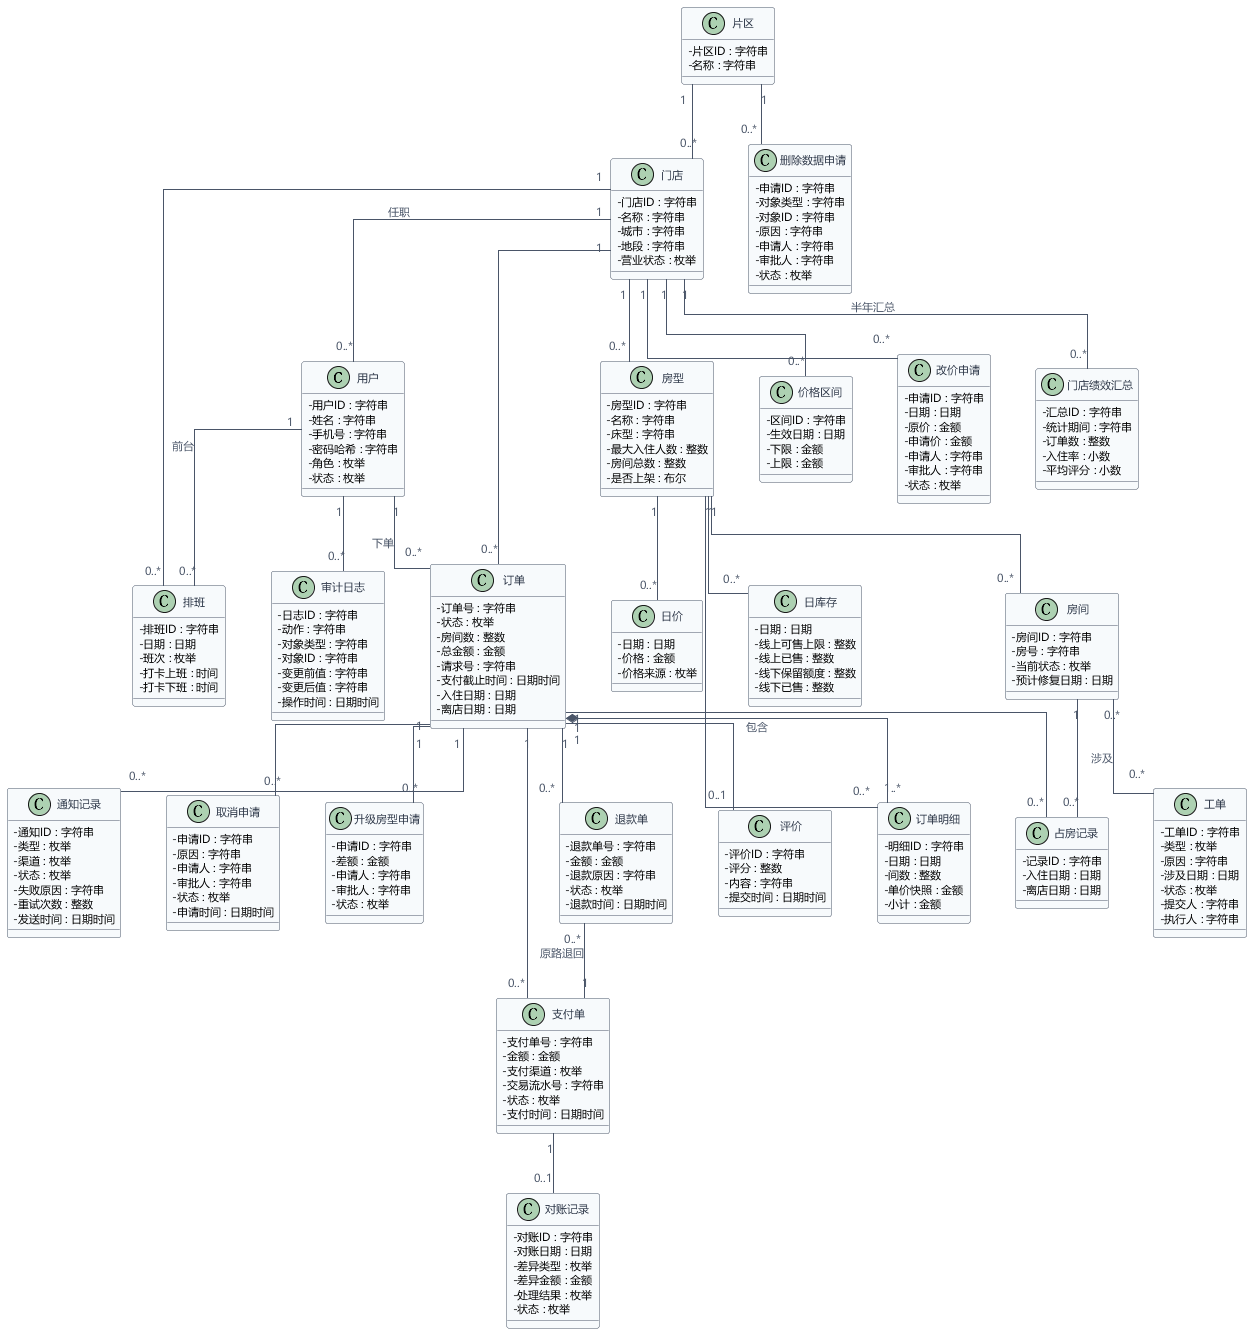
\includegraphics[width=0.94\textwidth]{../UML/UML类图.png}
\caption{UML 类图：领域模型}
\label{fig:class}
\end{figure}

类图上有 24 个类，按职责可以分成四簇：

\begin{itemize}
  \item \textbf{组织与人员}：片区、门店、用户、排班。片区 1 对多门店，门店 1 对多用户与排班。
  \item \textbf{房源与价格}：房型、房间、日价、日库存、价格区间、改价申请。房型 1 对多房间，也 1 对多日价与日库存。
  \item \textbf{交易}：订单、订单明细、支付单、退款单、取消申请、升级房型申请、占房记录。
  \item \textbf{支撑}：工单、评价、审计日志、通知记录、对账记录、删除数据申请、门店绩效汇总。
\end{itemize}

读这张图要注意三处\textbf{刻意}的连接，它们各自对应一条需求：

\textbf{一、日库存挂在房型上，不挂在房间上。} 类图里 `日库存` 与 `房型` 是一对多关系，与 `房间` 没有任何直接连线。这是 REQ-013 的直接表达：库存按房型与日期逐晚记录，下单时并不知道住哪间。

\textbf{二、订单与订单明细是组合关系，且明细上带单价快照。} `订单` 与 `订单明细` 之间是实心菱形（组合），意味着明细不能脱离订单存在；`订单明细` 有 `单价快照` 与 `小计` 两个属性，改价不回写（REQ-023）。

\textbf{三、占房记录是一个独立的关联类。} 订单与房间之间不是直接的多对多，而是通过 `占房记录` 关联，且这条记录带 `入住日期` 与 `离店日期`。原因是一间房在不同日期可以被不同订单占用，直接用多对多表达会丢掉时间维度。

还有两处容易漏的关系：`取消申请` 与 `订单` 是多对一（一张订单可能有多次取消申请，只有一条会通过），`退款单` 与 `支付单` 是多对一且注明「原路退回」（退款必须挂在原支付单上，否则不知道该退到哪个渠道）。

\subsection{行为图：四张用例图}

\begin{figure}[htbp]
\centering
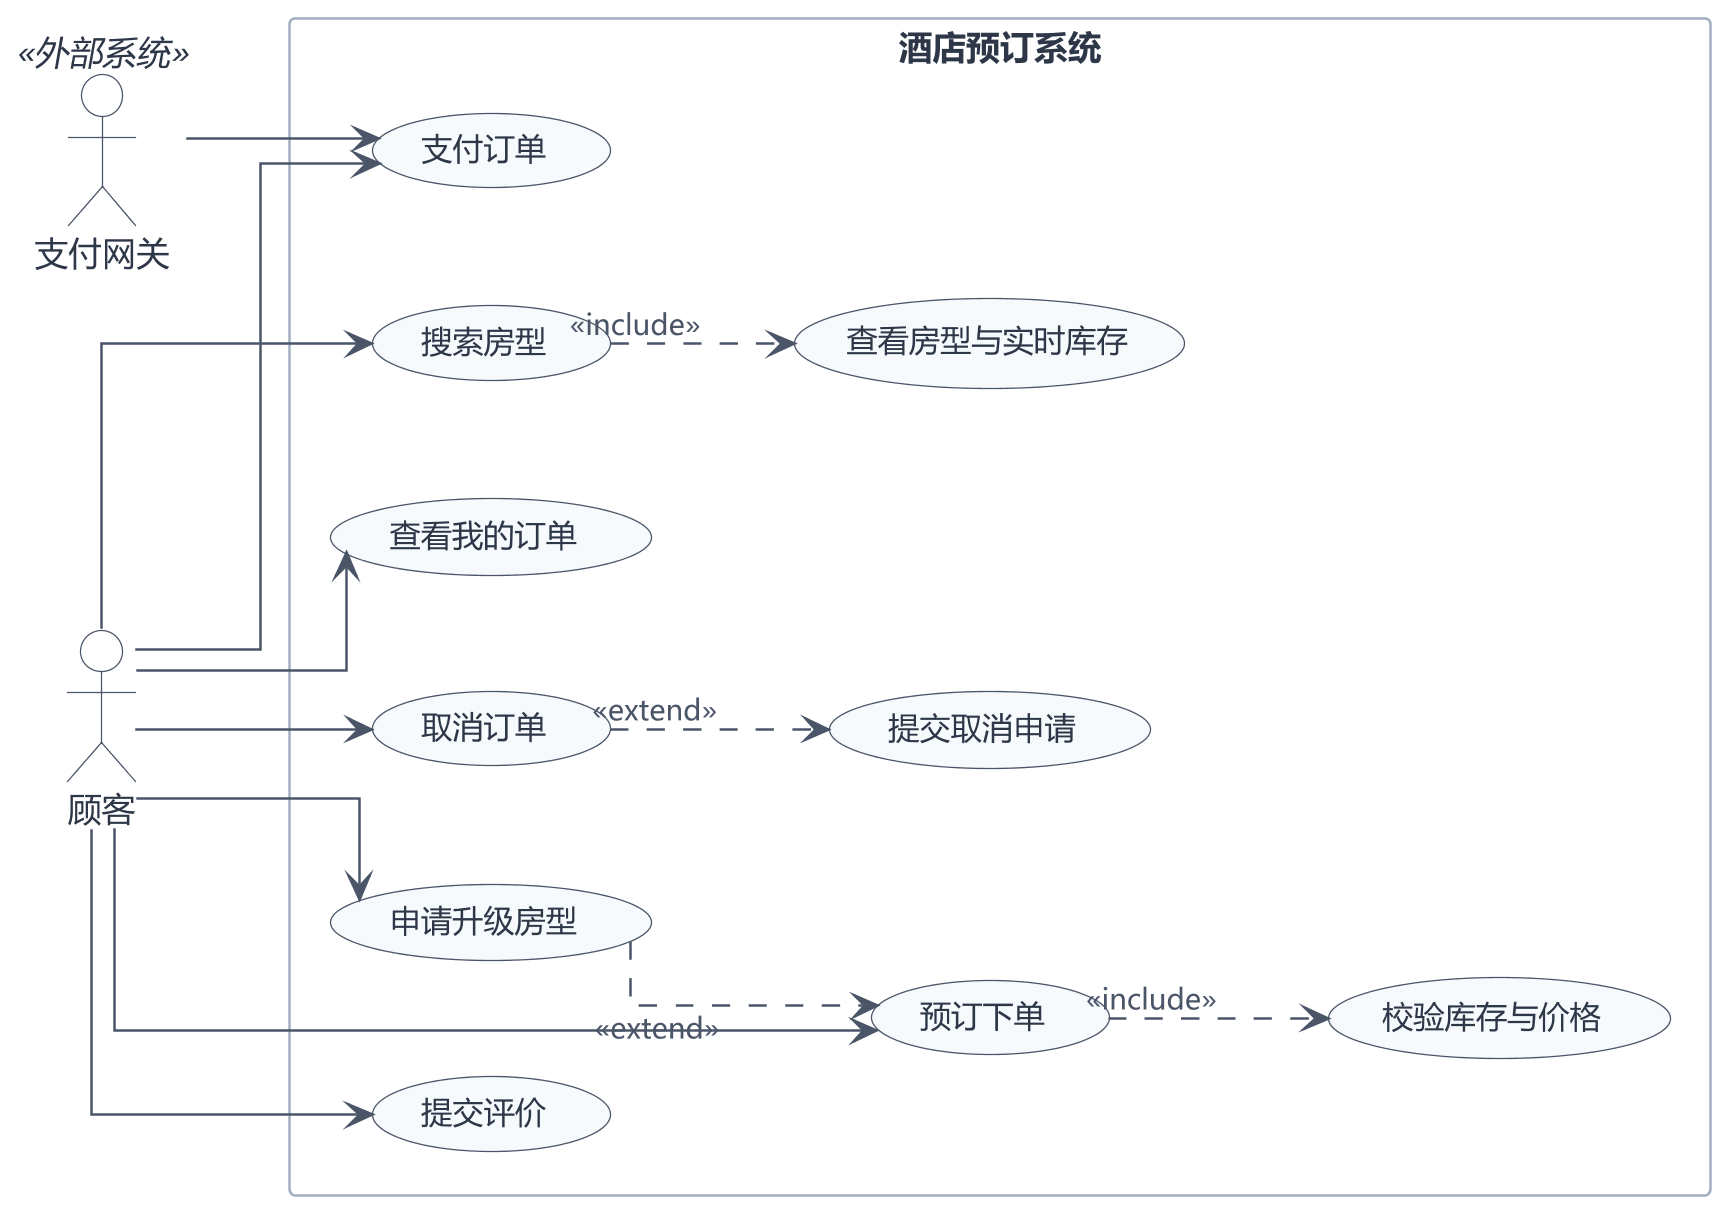
\includegraphics[width=0.86\textwidth]{../UML/UML用例图_顾客端.png}
\caption{UML 用例图：顾客端}
\label{fig:uc_c}
\end{figure}

顾客端九个用例，两条 include、两条 extend。最值得注意的是 `取消订单` 与 `提交取消申请` 是 extend 关系而不是 include——因为 18:00 之前取消根本不经过申请，只有过了 18:00 才扩展出「提交申请」这一步（REQ-021）。这一处如果画成 include，就等于说顾客每次取消都要走审批，与需求直接矛盾。

\begin{figure}[htbp]
\centering
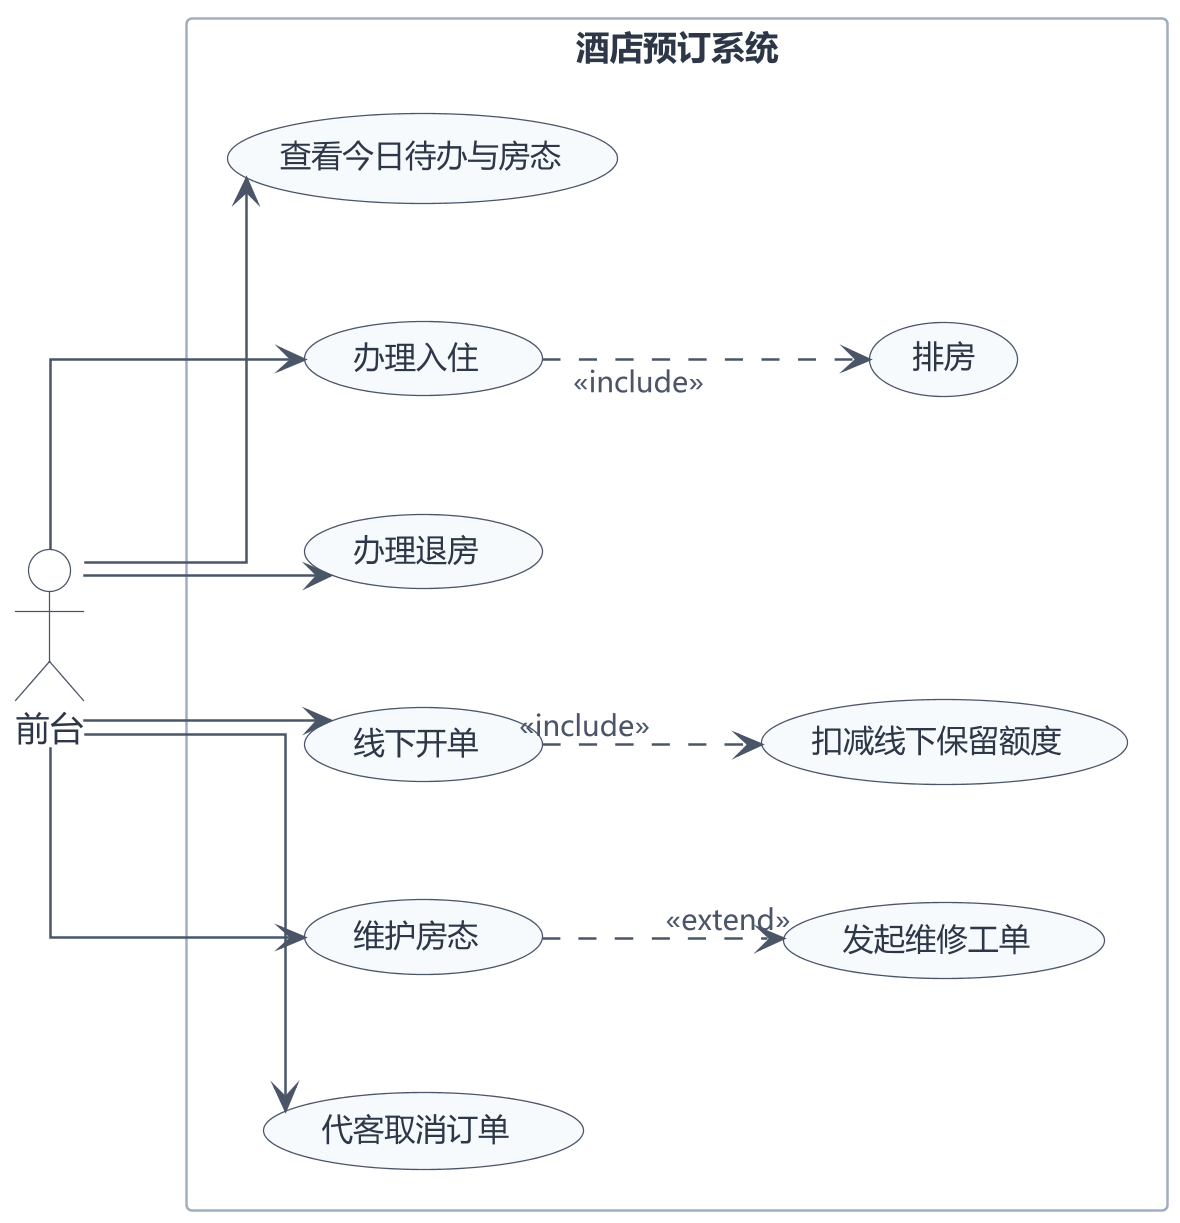
\includegraphics[width=0.86\textwidth]{../UML/UML用例图_前台端.png}
\caption{UML 用例图：前台端}
\label{fig:uc_f}
\end{figure}

前台端最关键的约束在图上是 `办理入住` include `排房`。这条 include 表达的是 REQ-018 的「3 步内完成」与 REQ-024 的「入住前必须排房」同时成立：入住一定伴随排房，但排房可以提前单独做（所以 `排房` 也是一个直接连到前台的用例）。

\begin{figure}[htbp]
\centering
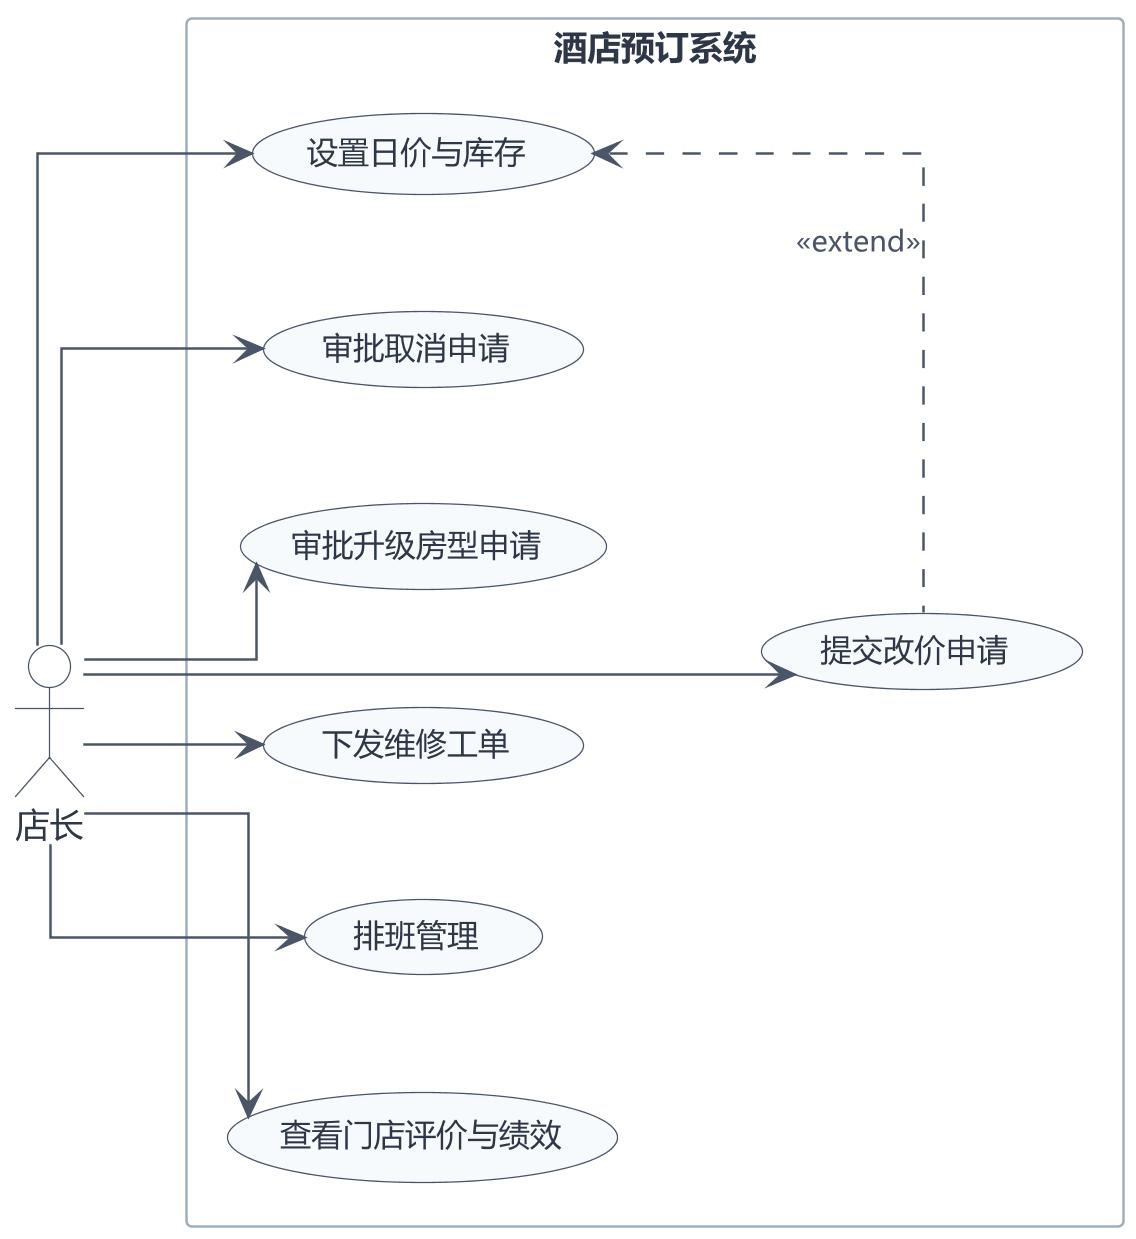
\includegraphics[width=0.8\textwidth]{../UML/UML用例图_店长端.png}
\caption{UML 用例图：店长端}
\label{fig:uc_s}
\end{figure}

店长端的 `提交改价申请` 与 `设置日价与库存` 之间是 extend：店长可以自己直接设价（在区间内），只有超区间时才扩展成「申请」再等审批。这解释了为什么店长自己发起的改价也要走审批中心——不是权限不够，而是留痕要求（REQ-014）。

\begin{figure}[htbp]
\centering
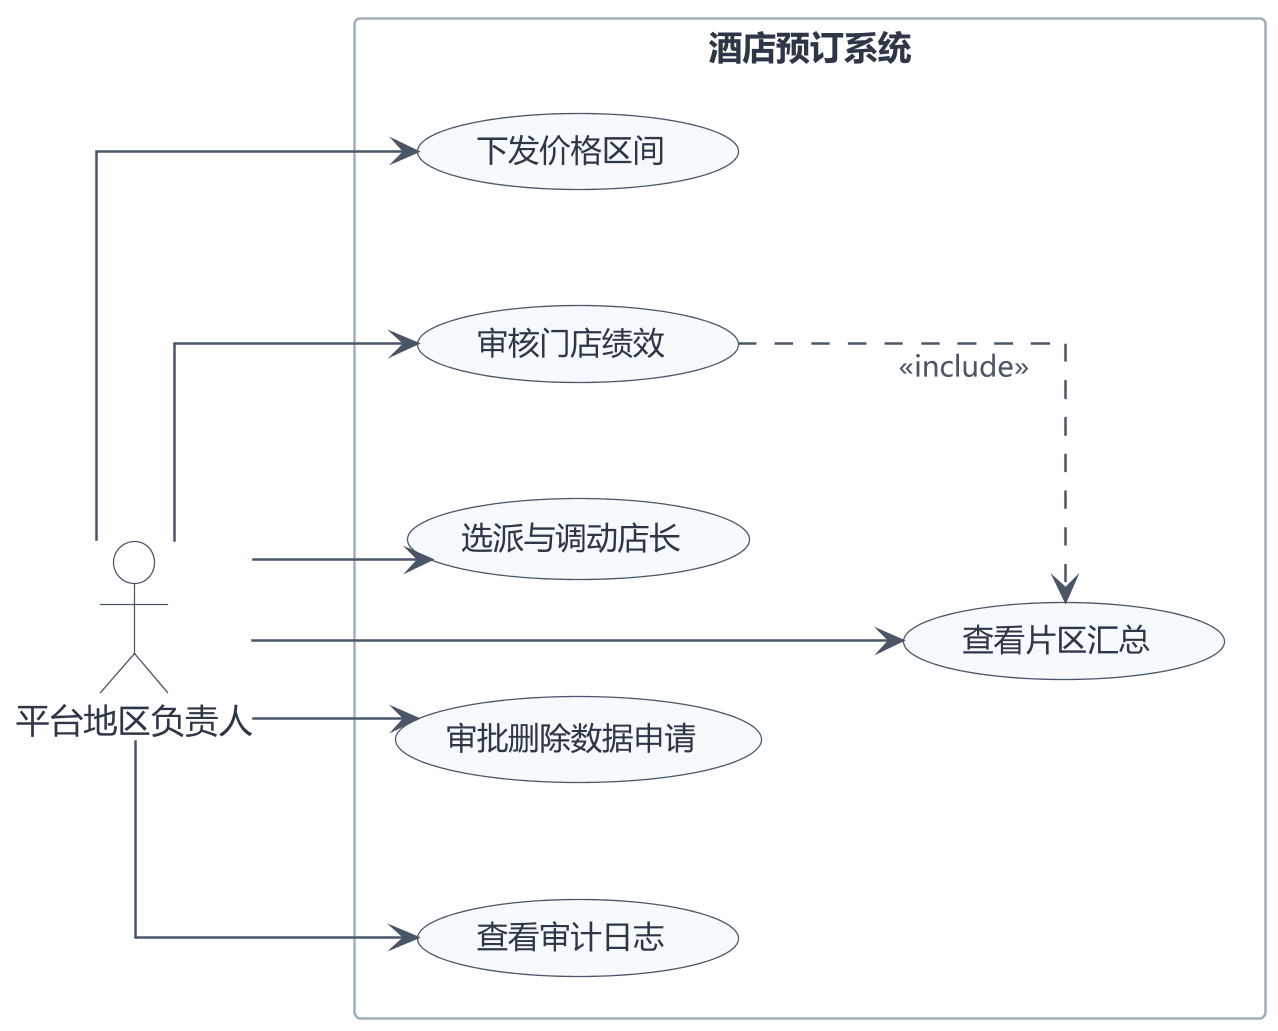
\includegraphics[width=0.8\textwidth]{../UML/UML用例图_平台端.png}
\caption{UML 用例图：平台端}
\label{fig:uc_p}
\end{figure}

平台端六个用例，`审核门店绩效` include `查看片区汇总`——审核绩效必须先看汇总，这不是可选项。图中没有「办理入住」「改房态」这类用例，是刻意的：REQ-007 明确平台地区负责人不得代门店办理业务。

\subsection{行为图：两台状态机}

\begin{figure}[htbp]
\centering
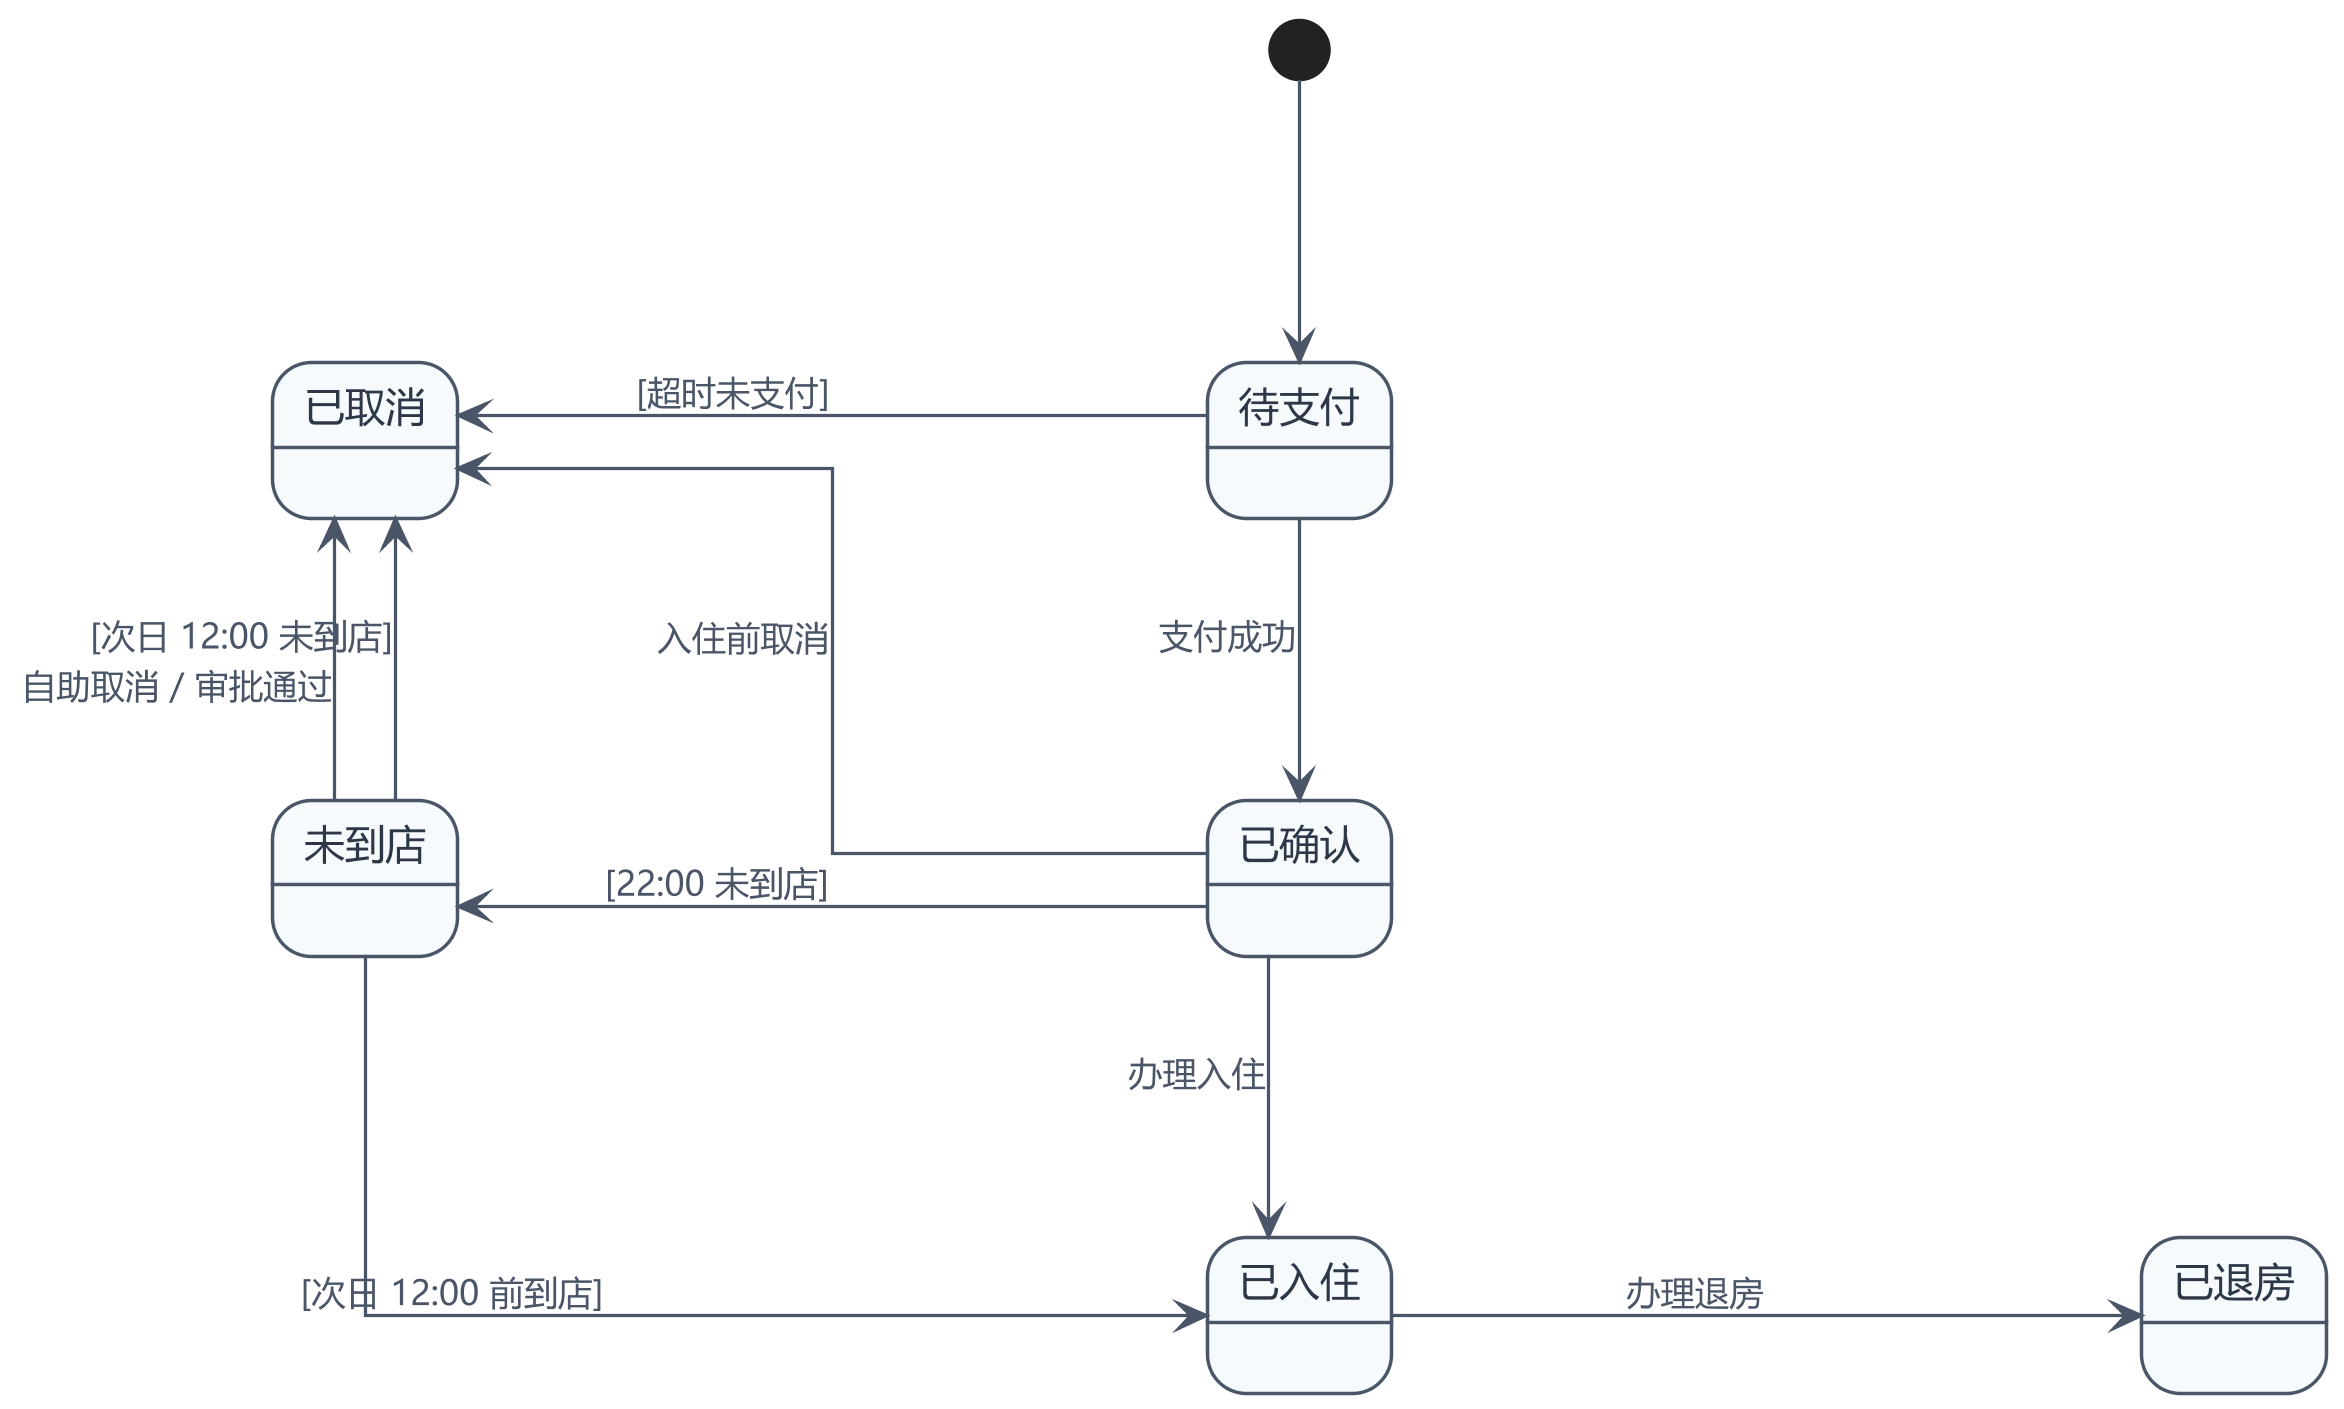
\includegraphics[width=0.82\textwidth]{../UML/UML状态图_订单.png}
\caption{UML 状态图：订单六态}
\label{fig:st_order}
\end{figure}

订单状态机的六条边里有两条带时间条件：`已确认 $\rightarrow$ 未到店` 的条件是「22:00 未到店」，`未到店 $\rightarrow$ 已取消` 的条件是「次日 12:00 仍未到店」。这两条不是业务动作触发的，是定时任务触发的，因此在状态图上用方括号条件标注，与「支付成功」「办理入住」这类动作边区分开。

对应的状态转换表如下（非法转换统一抛异常，不做「尽力修正」）：

\begin{table}[H]
\centering
\caption{订单状态转换表}
\tabfont
\begin{tabularx}{\textwidth}{@{}L{2.1cm}L{2.1cm}L{3.3cm}X@{}}
\toprule
当前状态 & 目标状态 & 触发 & 说明 \\
\midrule
（新建） & 待支付 & 顾客提交 & 同事务扣库存 \\
待支付 & 已确认 & 支付回调 & 条件更新，影响 1 行才继续 \\
待支付 & 已取消 & 超时任务 & 15 分钟未支付，同事务释放库存 \\
已确认 & 已入住 & 前台办理入住 & 与房间状态同步变更 \\
已确认 & 已取消 & 自助 / 审批通过 & 18:00 为界（REQ-021） \\
已确认 & 未到店 & 定时任务 & 入住日 22:00 \\
未到店 & 已入住 & 前台办理入住 & 仅限次日 12:00 前 \\
未到店 & 已取消 & 定时任务 & 次日 12:00，不退房费 \\
已入住 & 已退房 & 前台确认退房 & 与房间状态同步变更 \\
\midrule
\multicolumn{4}{@{}l}{\zihao{5}禁止：待支付 $\rightarrow$ 已入住 / 已退房 / 未到店；已确认 $\rightarrow$ 已退房；已入住 $\rightarrow$ 已取消 / 未到店；} \\
\multicolumn{4}{@{}l}{\zihao{5}未到店 $\rightarrow$ 已确认 / 已退房；已退房、已取消为终态；任何状态不得回到待支付。} \\
\bottomrule
\end{tabularx}
\end{table}

\begin{figure}[htbp]
\centering
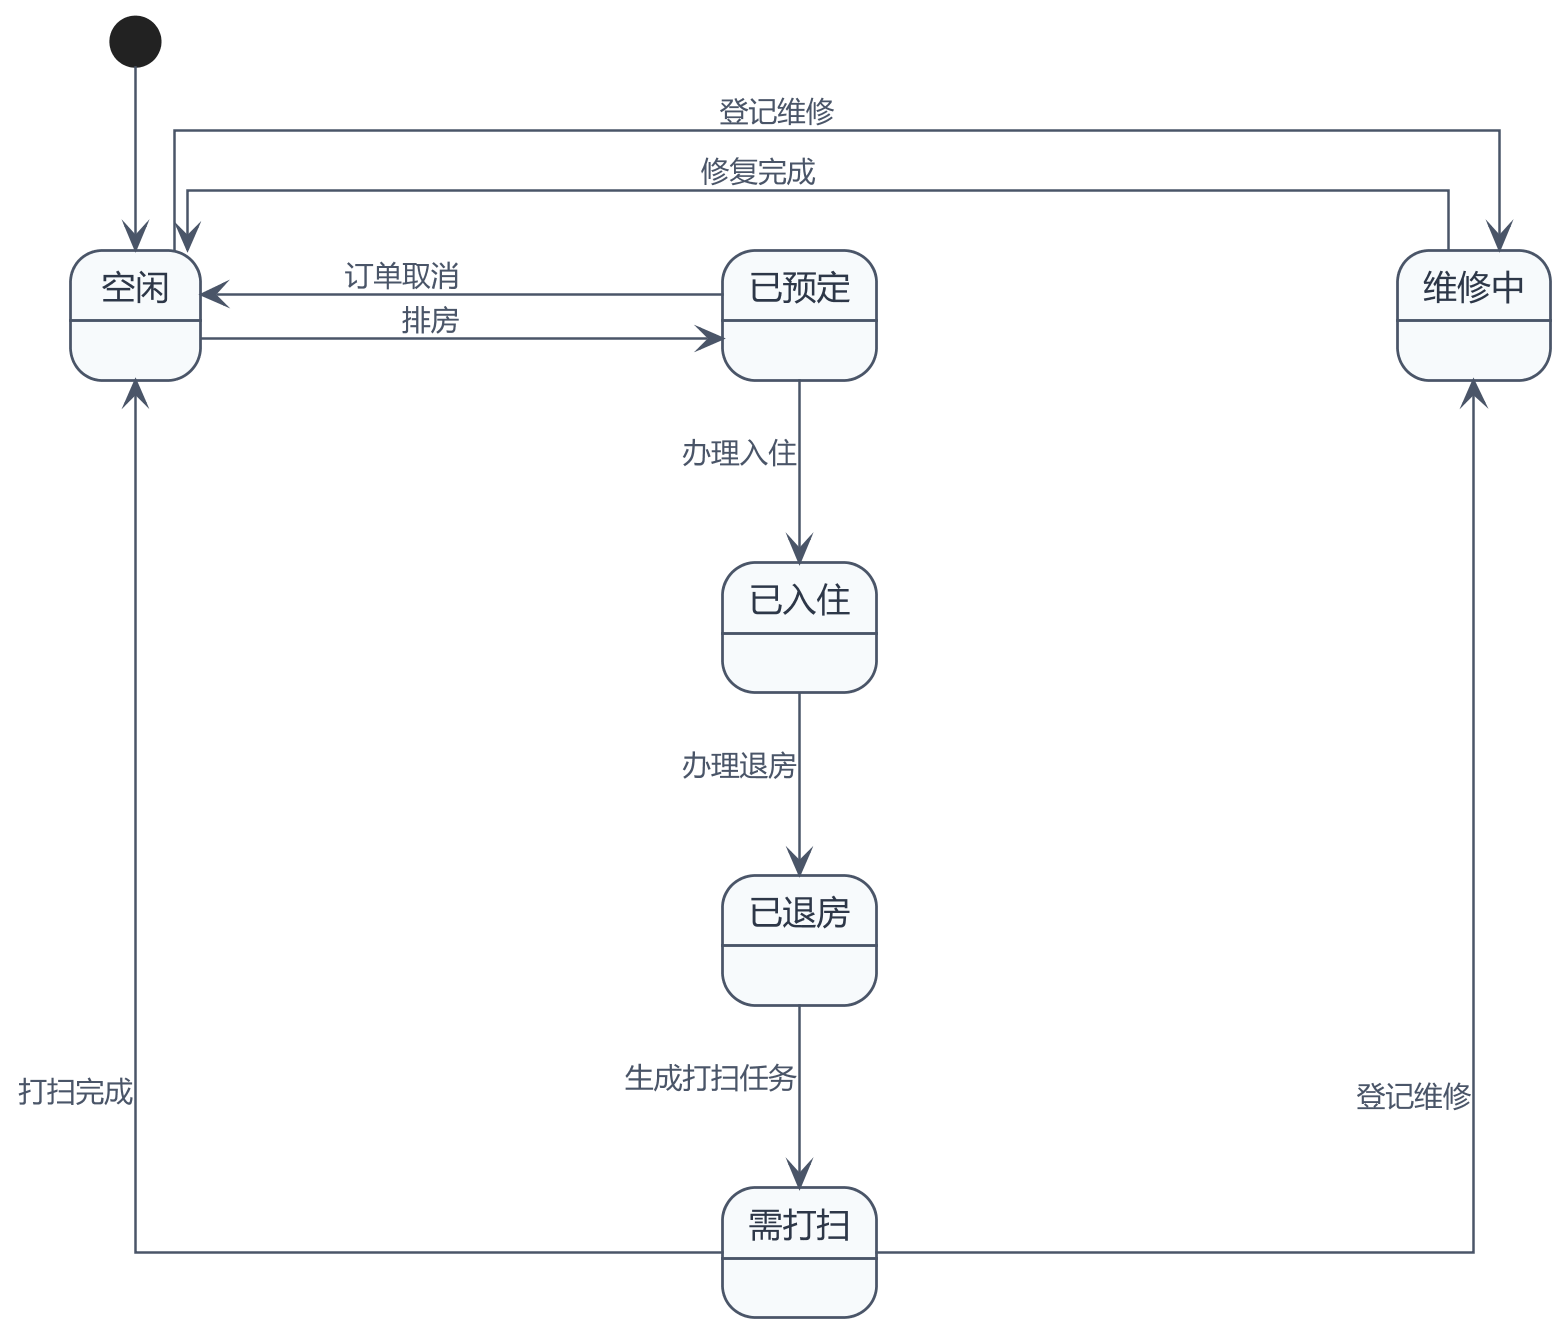
\includegraphics[width=0.78\textwidth]{../UML/UML状态图_房间.png}
\caption{UML 状态图：房间六态}
\label{fig:st_room}
\end{figure}

房间状态机比订单多一条旁路：维修中。它可以从「空闲」进入，也可以从「需打扫」进入，修复后回到「空闲」。这条旁路的意义在 REQ-034——房间转维修时，按维修日期逐日从该房型可售上限中扣除，修复当日起恢复。房态图上没有「维修中 $\rightarrow$ 已入住」这条边，是因为维修中的房间不允许排房，这一点在 REQ-024 的异常情况里写着。

\subsection{行为图：两张活动图}

\begin{figure}[htbp]
\centering
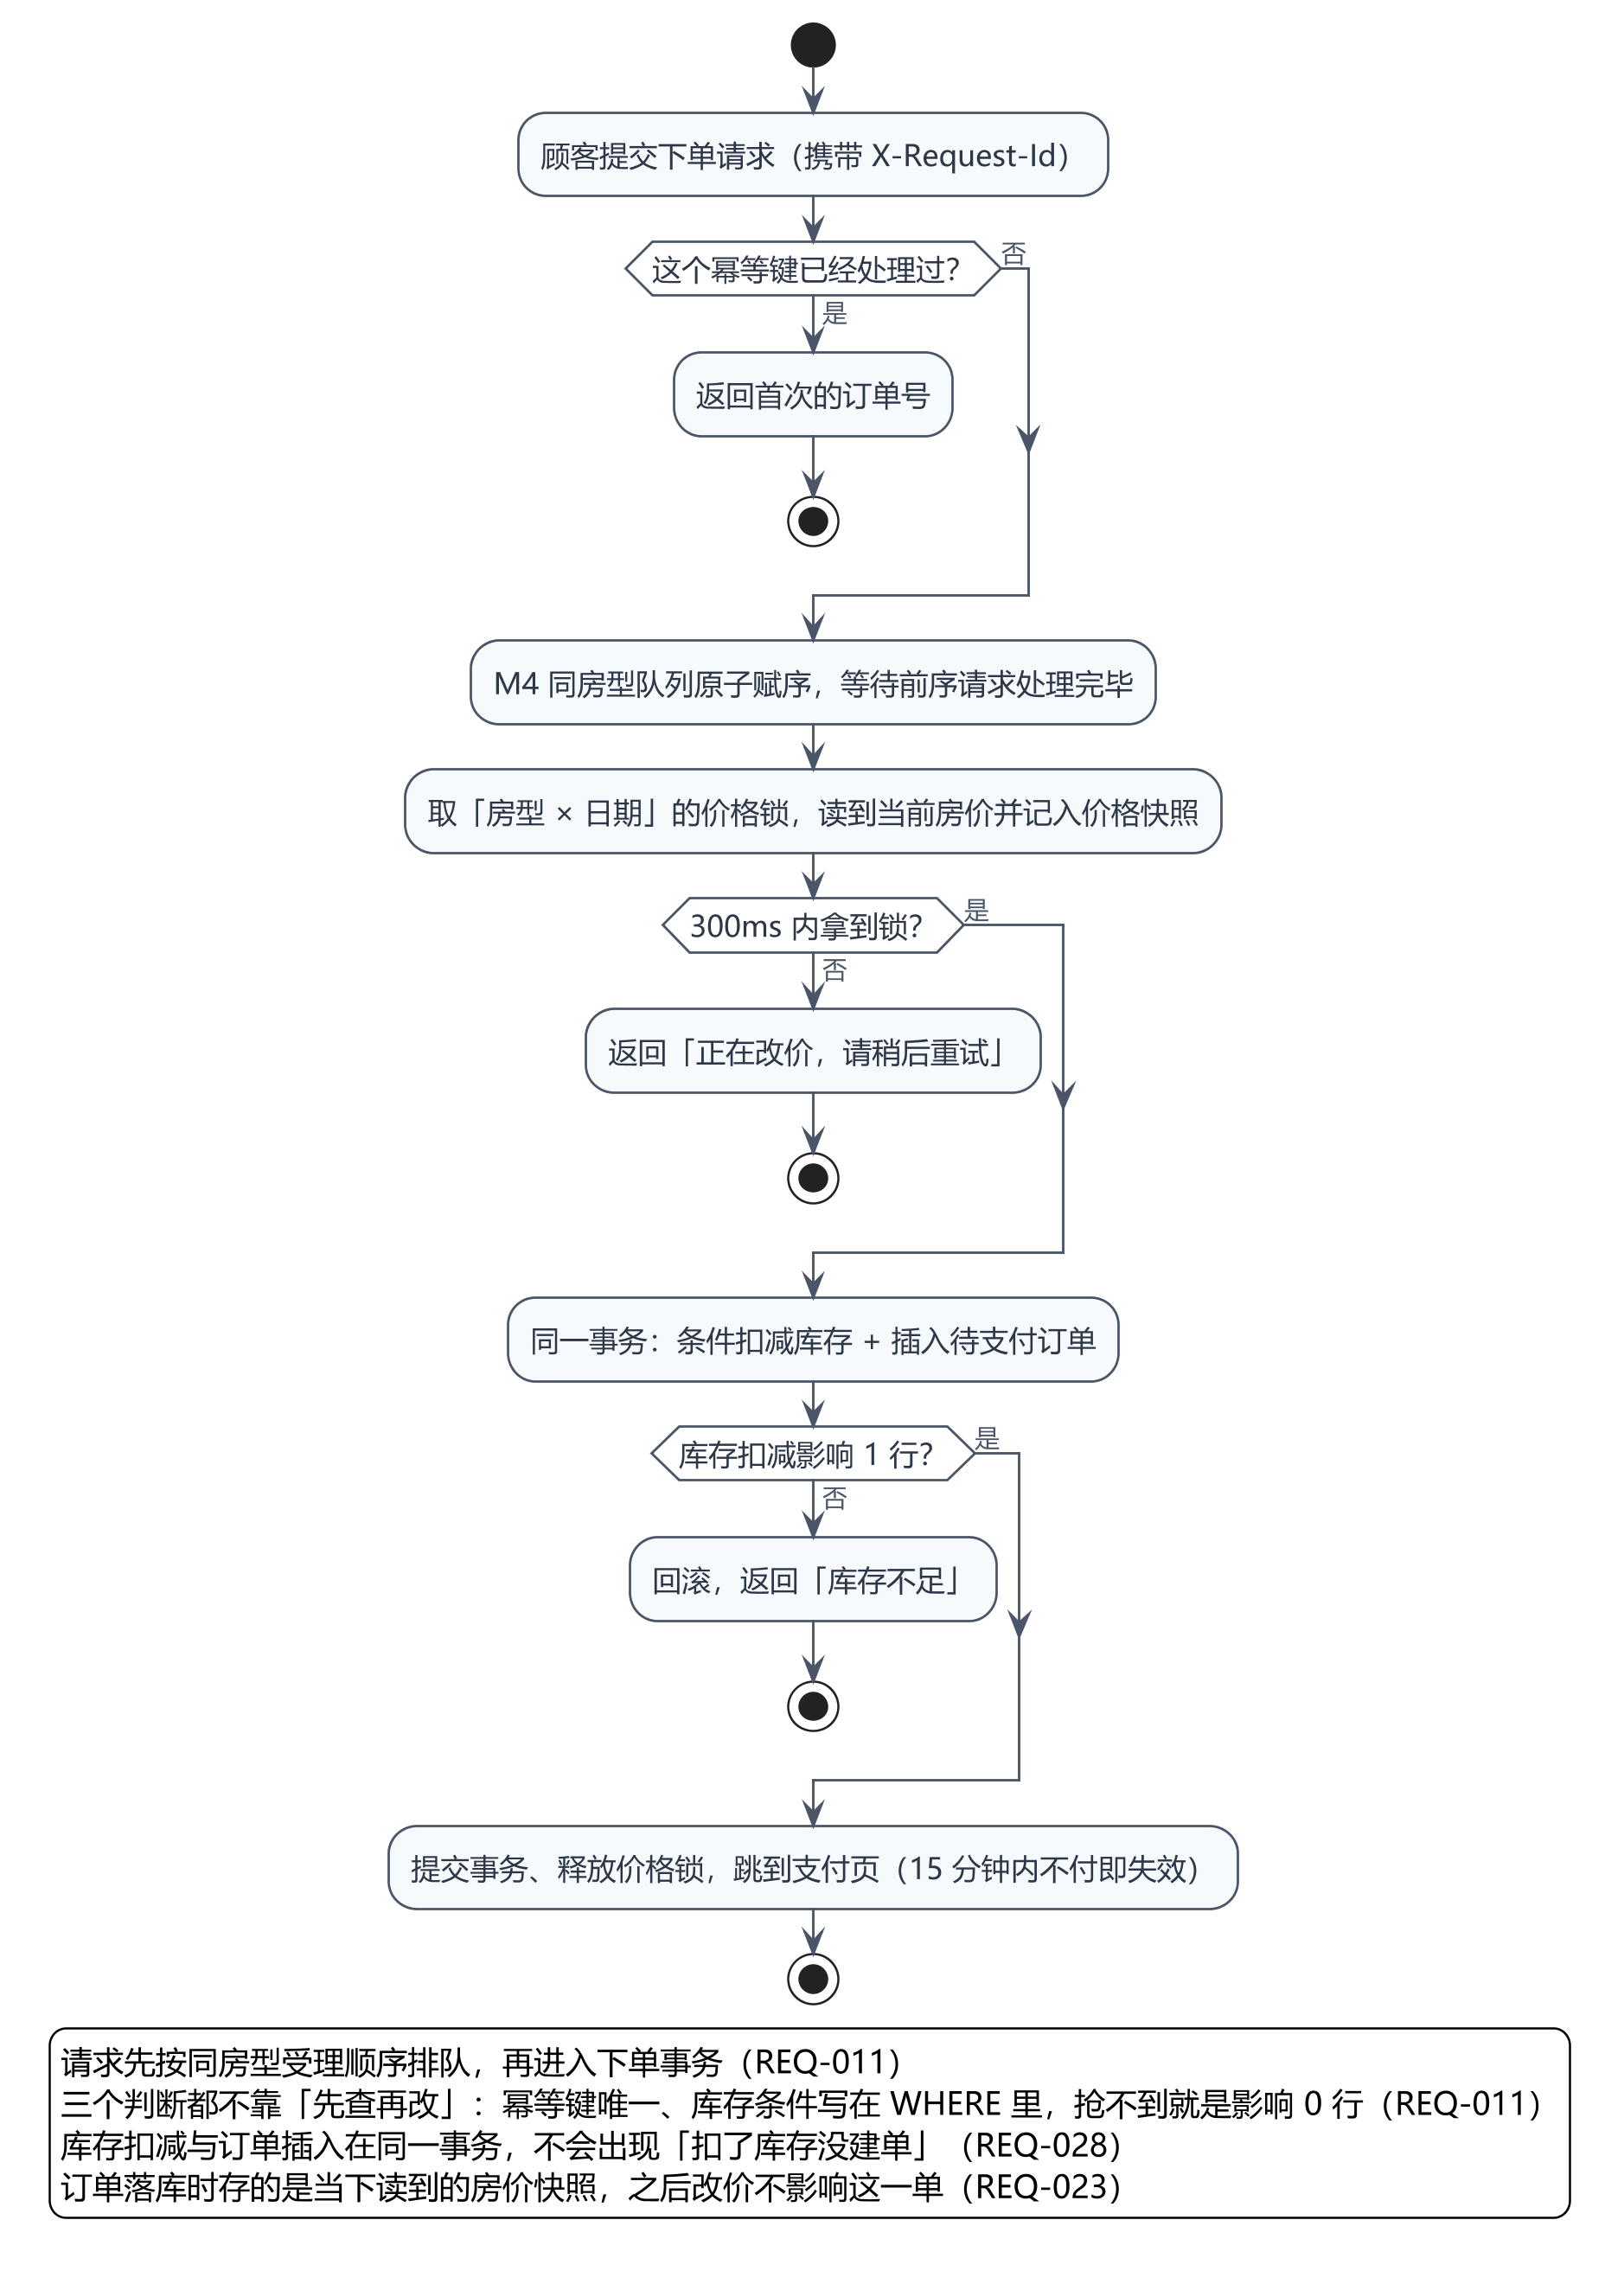
\includegraphics[width=0.62\textwidth]{../UML/UML活动图_下单与锁库存.png}
\caption{UML 活动图：下单与锁库存}
\label{fig:act1}
\end{figure}

下单活动图上有三个菱形判断，每一个都对应一种「不这么写就会出事」的场景：

\begin{enumerate}[leftmargin=3.2em]
  \item \textbf{幂等键是否已经处理过？} 是则直接返回首次的订单号，不新建订单（REQ-010）。
  \item \textbf{300 ms 内拿到价格锁了吗？} 否则返回「正在改价，请稍后重试」，\textbf{不静默用旧价}（REQ-012）。
  \item \textbf{库存条件扣减影响 1 行了吗？} 否则回滚并返回库存不足，不落任何订单（REQ-011）。
\end{enumerate}

三个判断的共同设计取向是：\textbf{失败要显式失败，不能退化成「差不多成功」}。把锁超时退化成用旧价、把库存不足退化成排队重试，都会在事后变成「订单金额不对」或「到店无房」这类无法解释的问题。

% 在进入本节前清空浮动队列，否则后续四张时序图会被推到一起、与说明文字脱节
\clearpage
\begin{figure}[htbp]
\centering
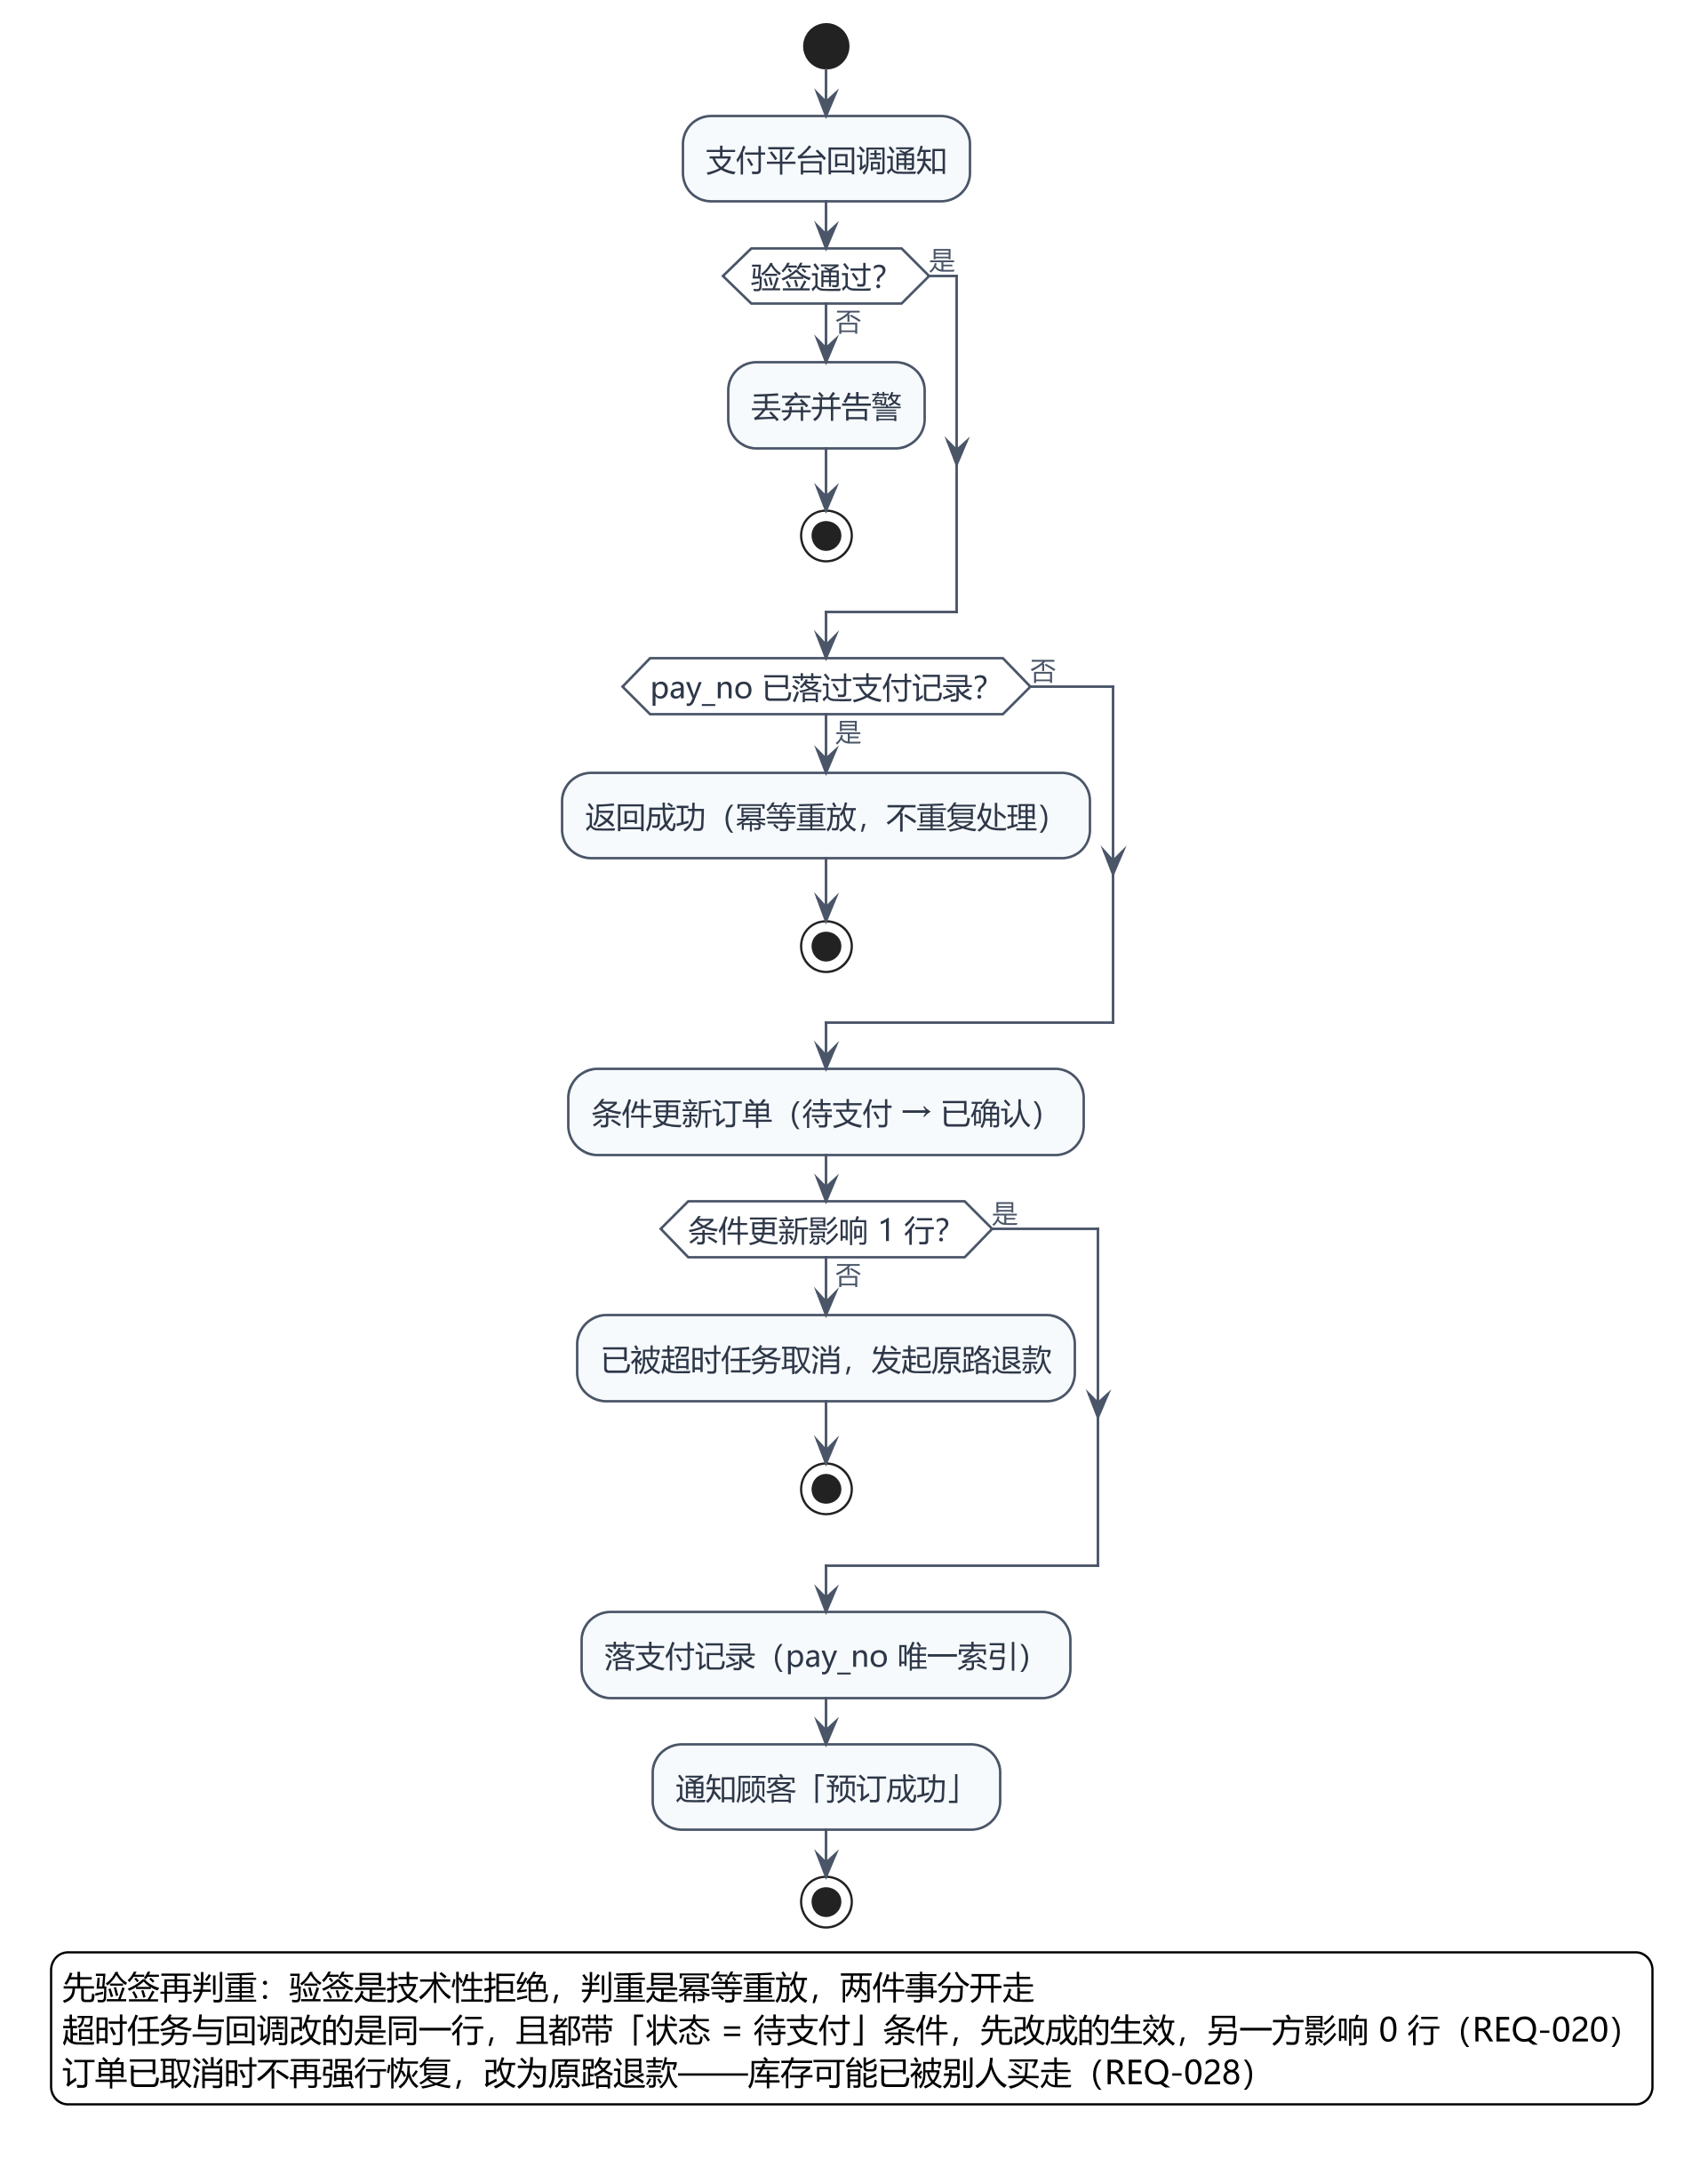
\includegraphics[width=0.62\textwidth]{../UML/UML活动图_支付回调与订单生效.png}
\caption{UML 活动图：支付回调与订单生效}
\label{fig:act2}
\end{figure}

支付回调活动图上的判断顺序是有讲究的：\textbf{先验签，再判重，最后看订单状态}。验签失败是技术性拒绝（可能是伪造请求），判重命中是正常的幂等重放（支付平台会重发），两者的日志级别、告警策略、返回码都不同，因此不能合并成一个判断。最后一步按订单\textbf{此刻}的状态分叉——已成已取消就退款而不是恢复订单，这是 REQ-028 的核心。

\subsection{交互图：四张时序图}

\begin{figure}[htbp]
\centering
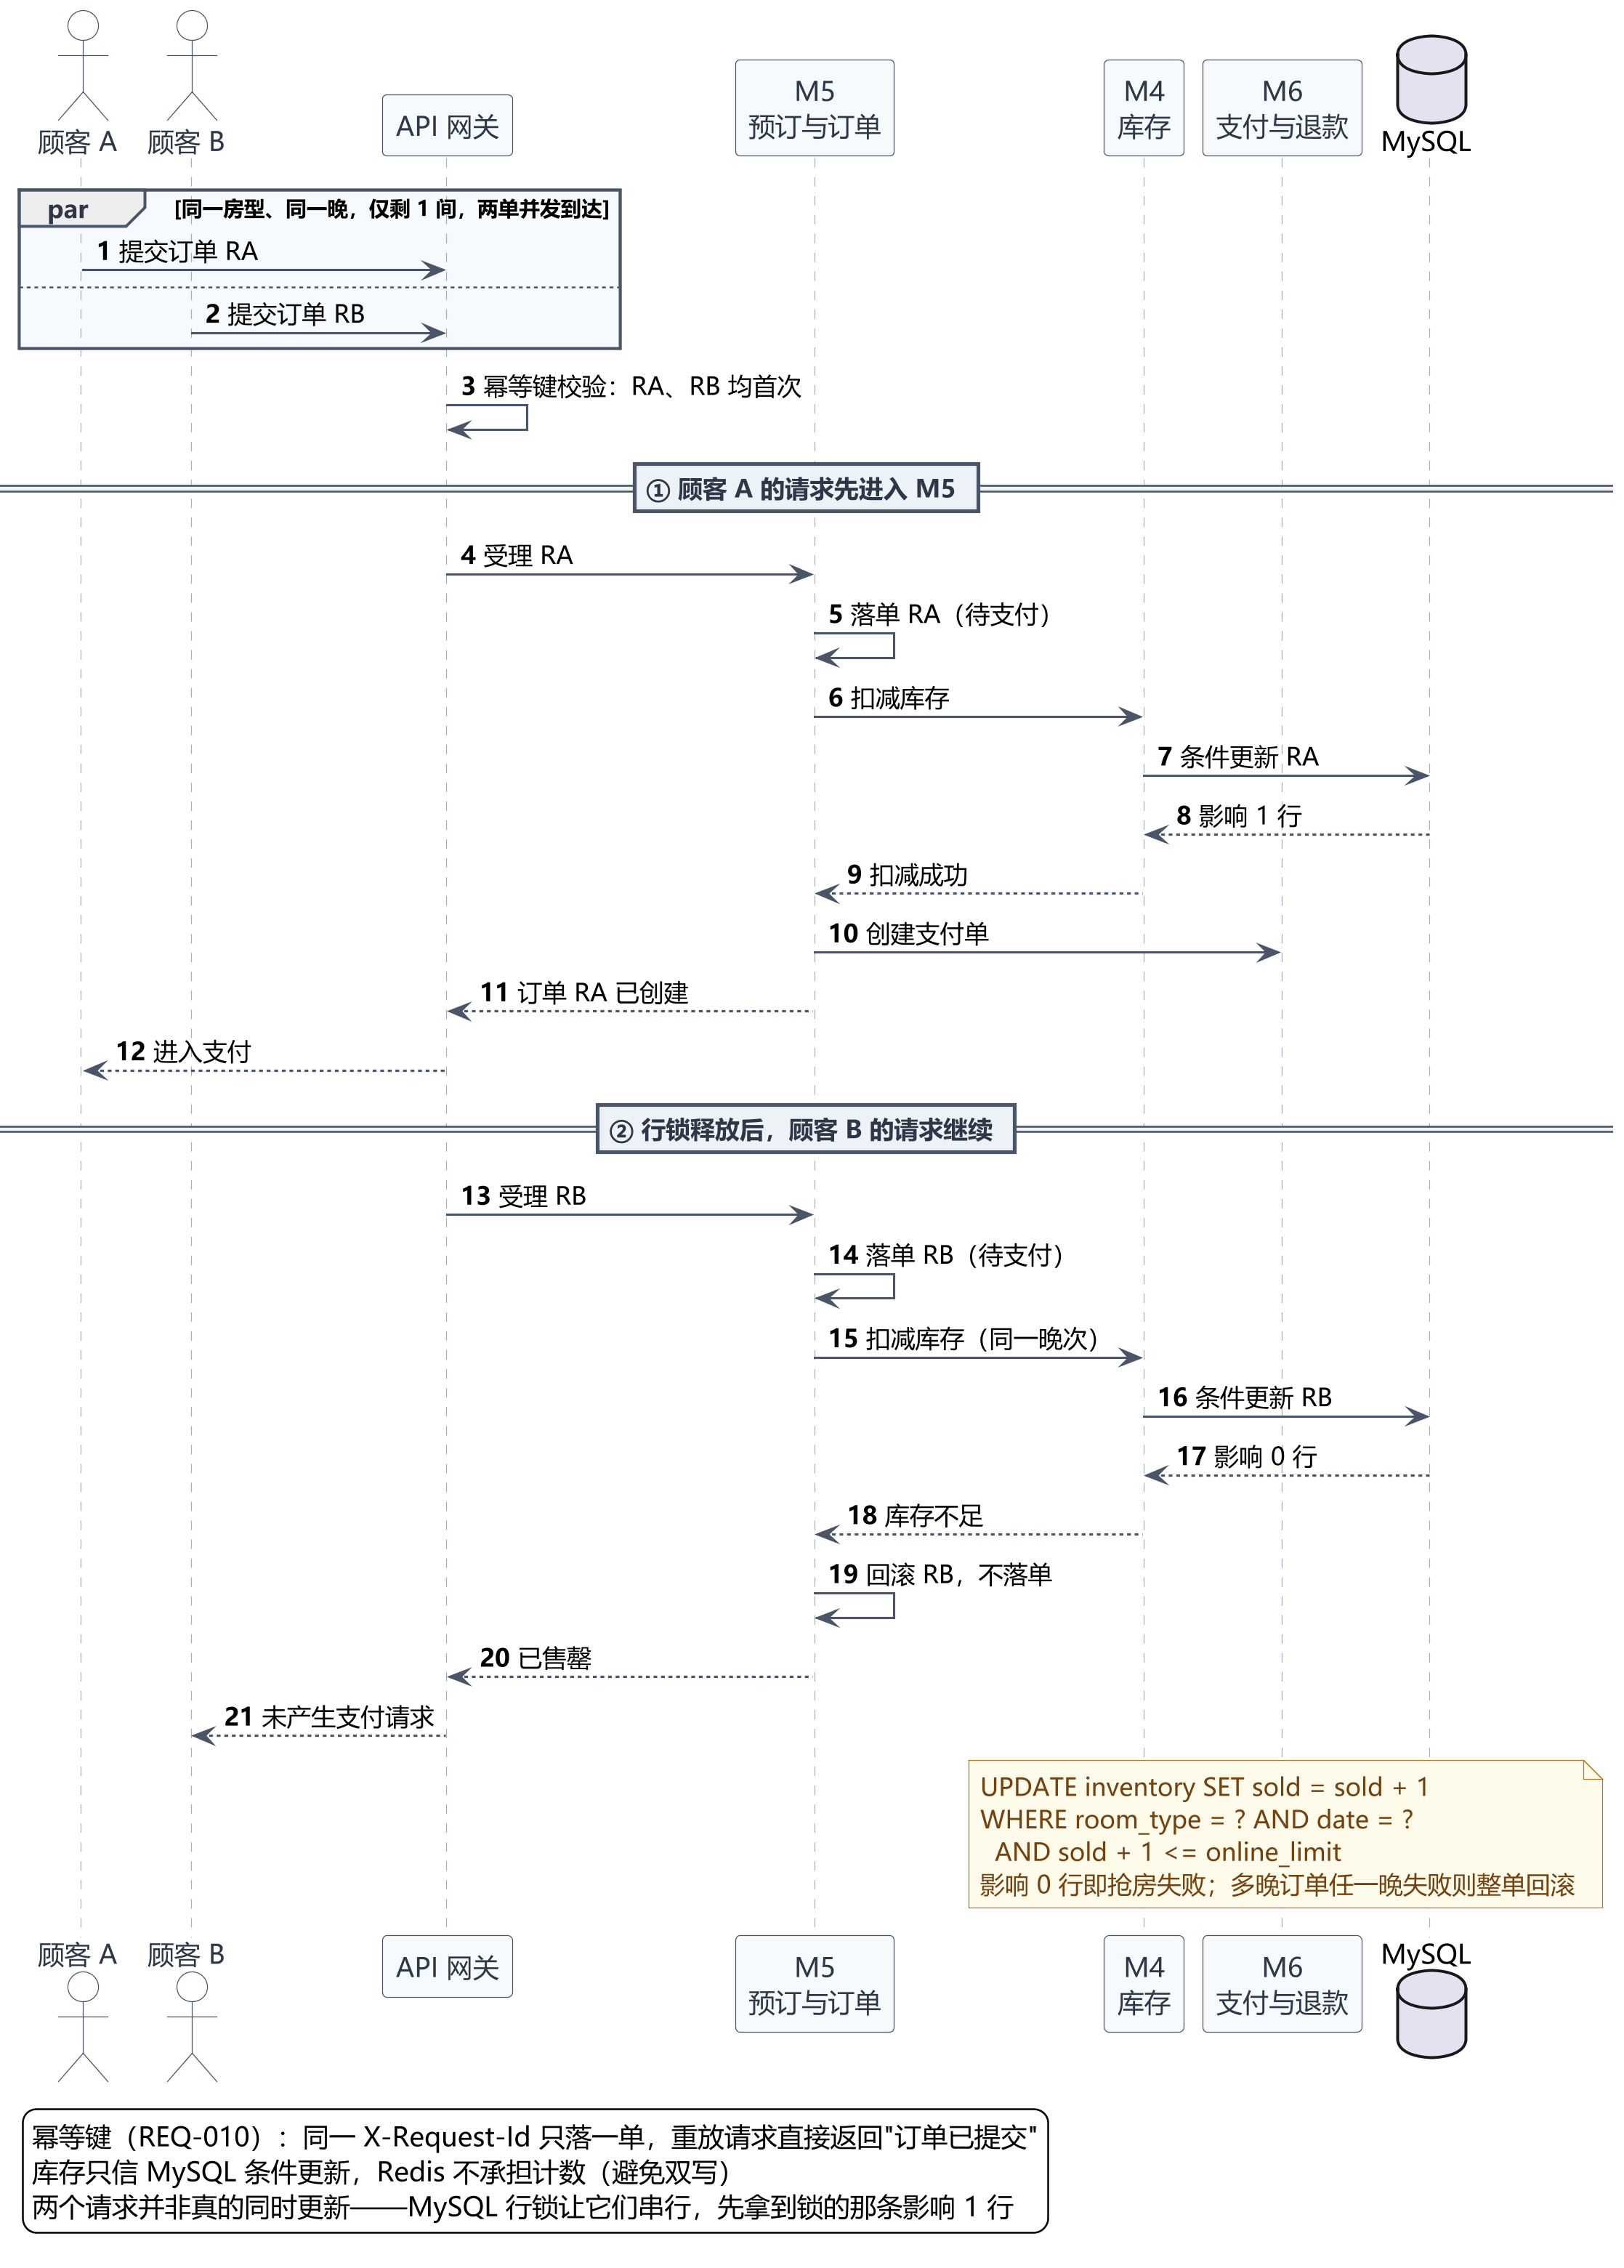
\includegraphics[width=0.68\textwidth]{../UML/UML时序图_并发抢房.png}
\caption{UML 时序图：并发抢房}
\label{fig:seq1}
\end{figure}

这张图想说明的是：所谓「并发」，在数据库层面其实是串行的。顾客 A 与 B 的请求同时到达，但两次 UPDATE 之间隔着 MySQL 的行锁，先拿到锁的那条影响 1 行，后一条影响 0 行。因此「按服务端收到提交的时间排序，最先成功者获得库存」（REQ-011）不需要额外的排序逻辑，行锁的获取顺序就是实际顺序。

同时这张图上还有一条容易忽略的线：顾客 B 抢房失败后\textbf{不产生支付请求}。这是需求里明写的边界——抢房失败却生成了支付单，就会出现「付了钱但没有房」的对账差异。

\begin{figure}[htbp]
\centering
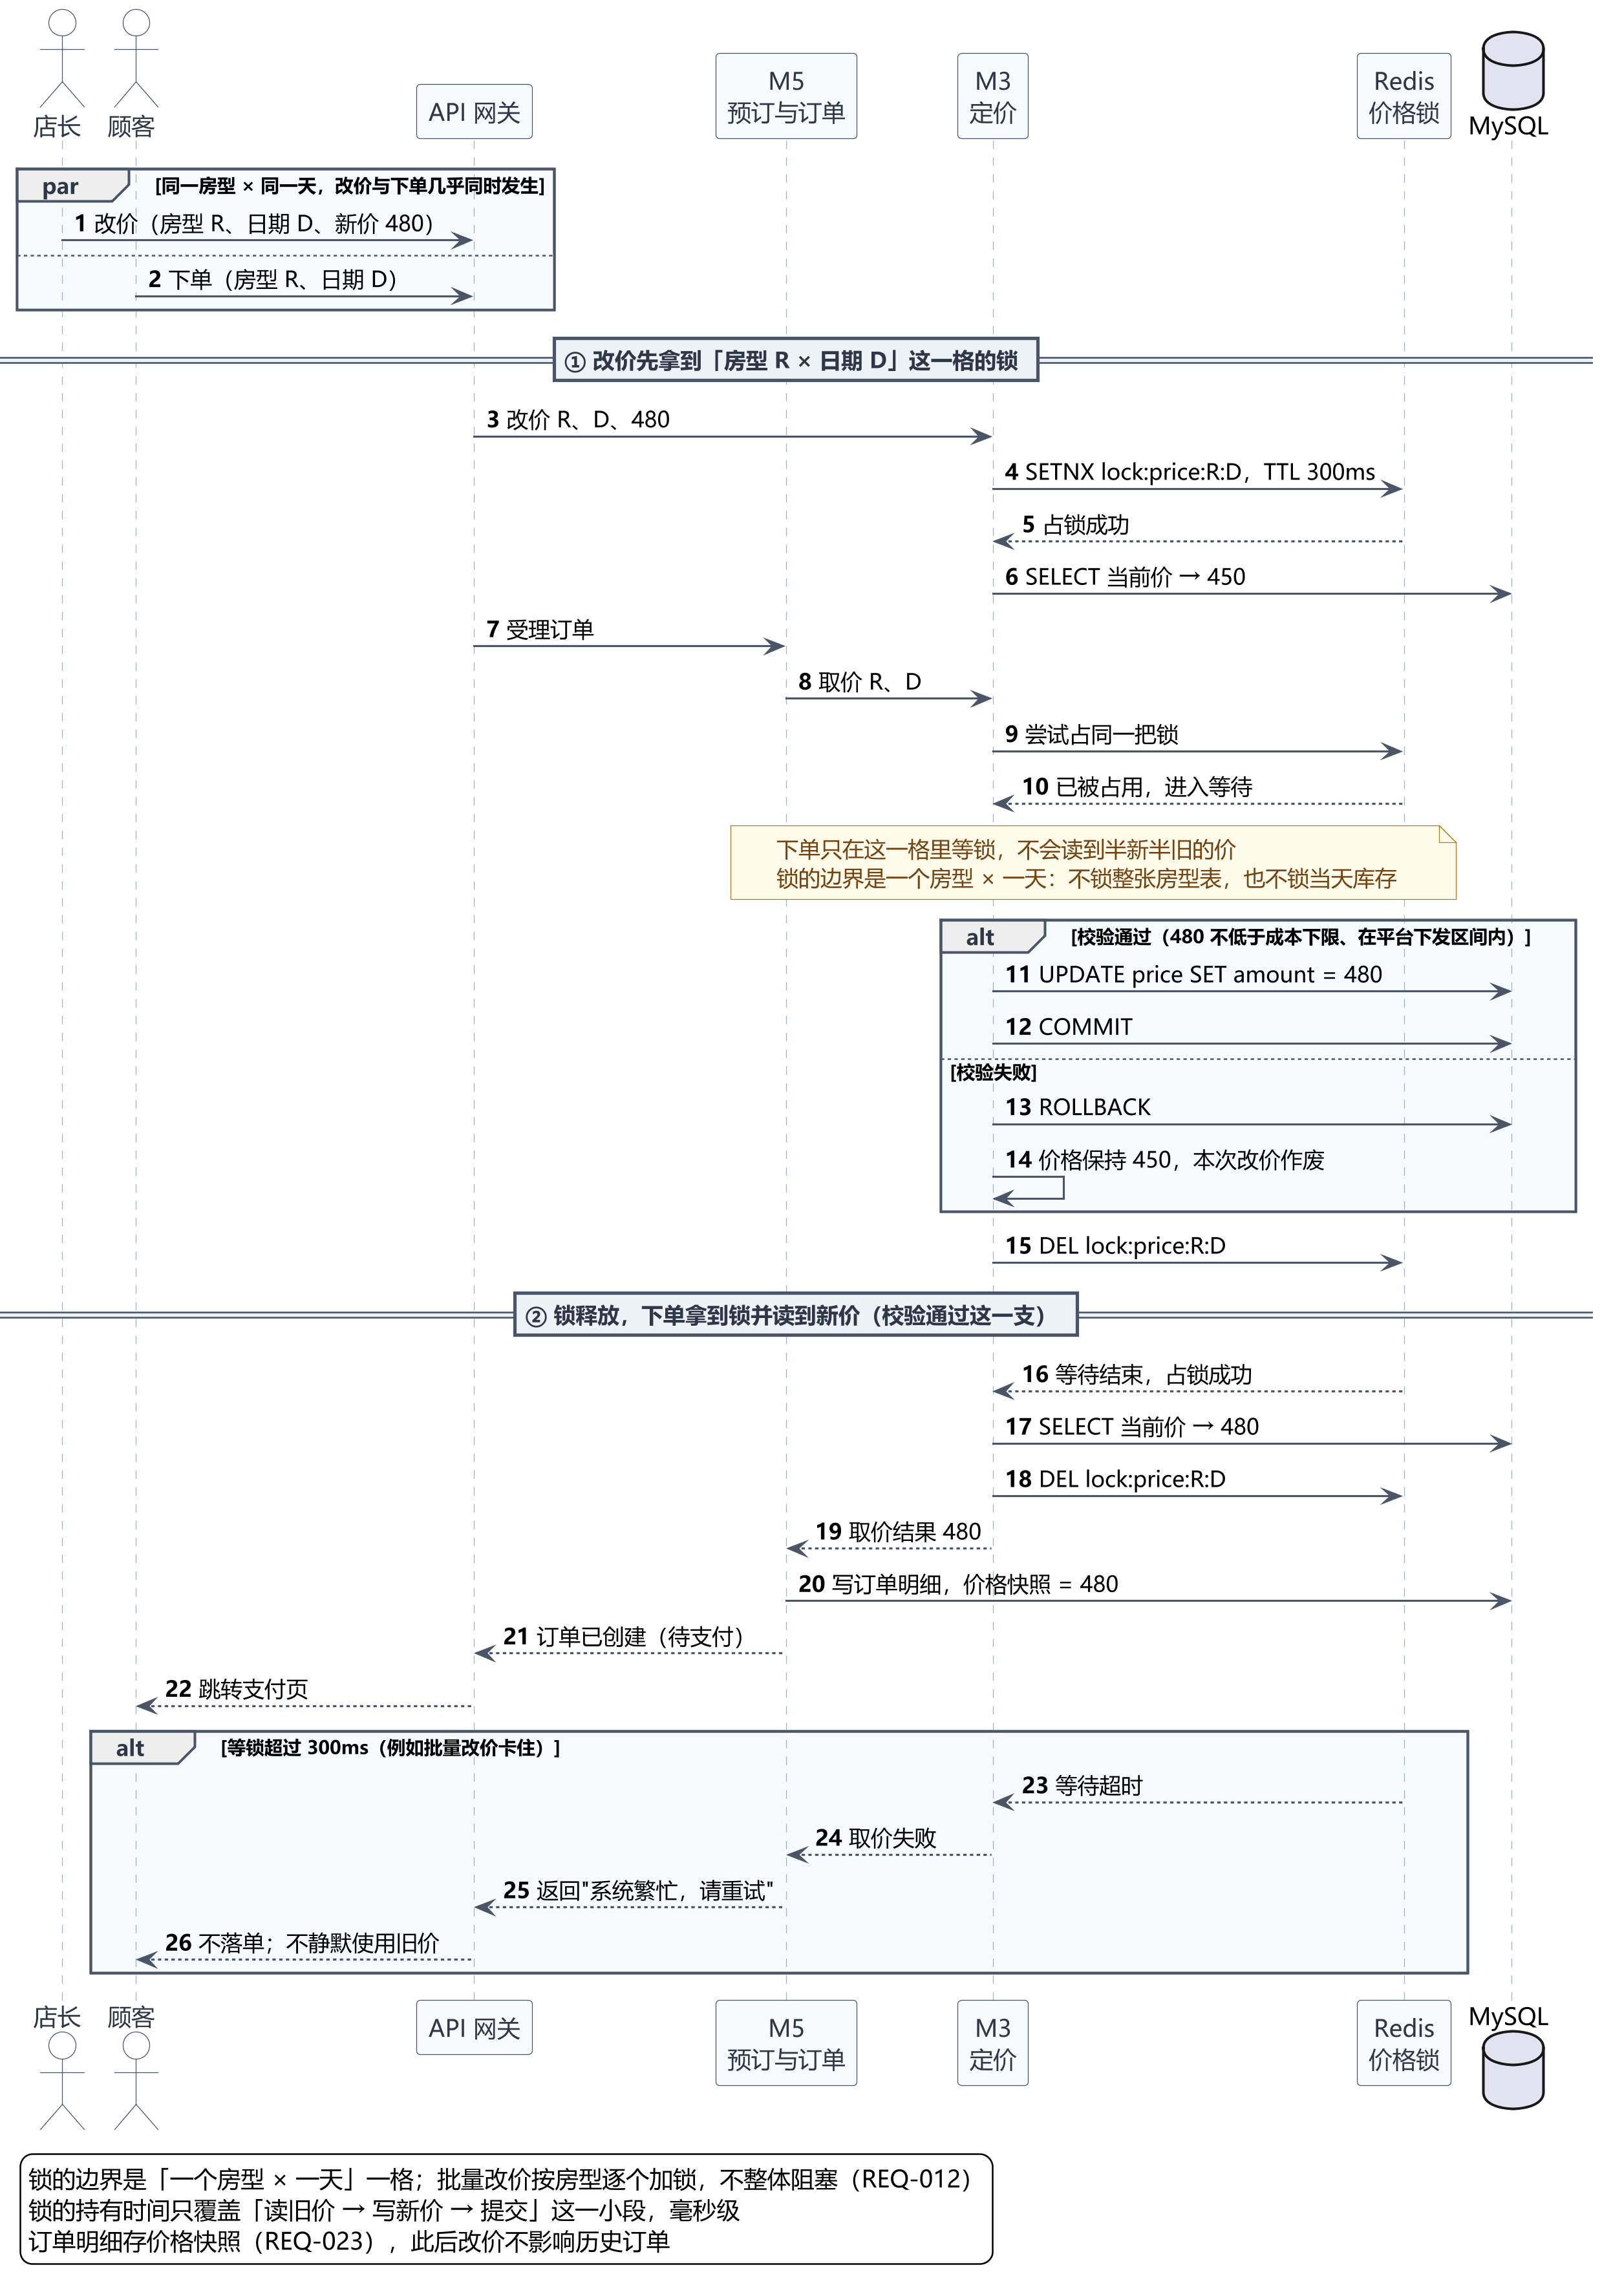
\includegraphics[width=0.68\textwidth]{../UML/UML时序图_改价互斥.png}
\caption{UML 时序图：改价与下单互斥}
\label{fig:seq2}
\end{figure}

改价互斥这张图最需要说明的是\textbf{锁的边界}。锁的粒度是「一个房型 $\times$ 一天」，不是整张房型表，也不是当天库存。批量改十个房型时按房型逐个加锁，不整体阻塞下单。锁的持有时间只覆盖「读旧价 $\rightarrow$ 写新价 $\rightarrow$ 提交」这一小段，毫秒级。

图的下半部分还有一条容易被忽略的分支：等锁超过 300 ms 时返回「系统繁忙，请重试」，订单不落库。这说明锁超时不是「降级使用旧价」，而是「明确告诉用户再来一次」。

\begin{figure}[htbp]
\centering
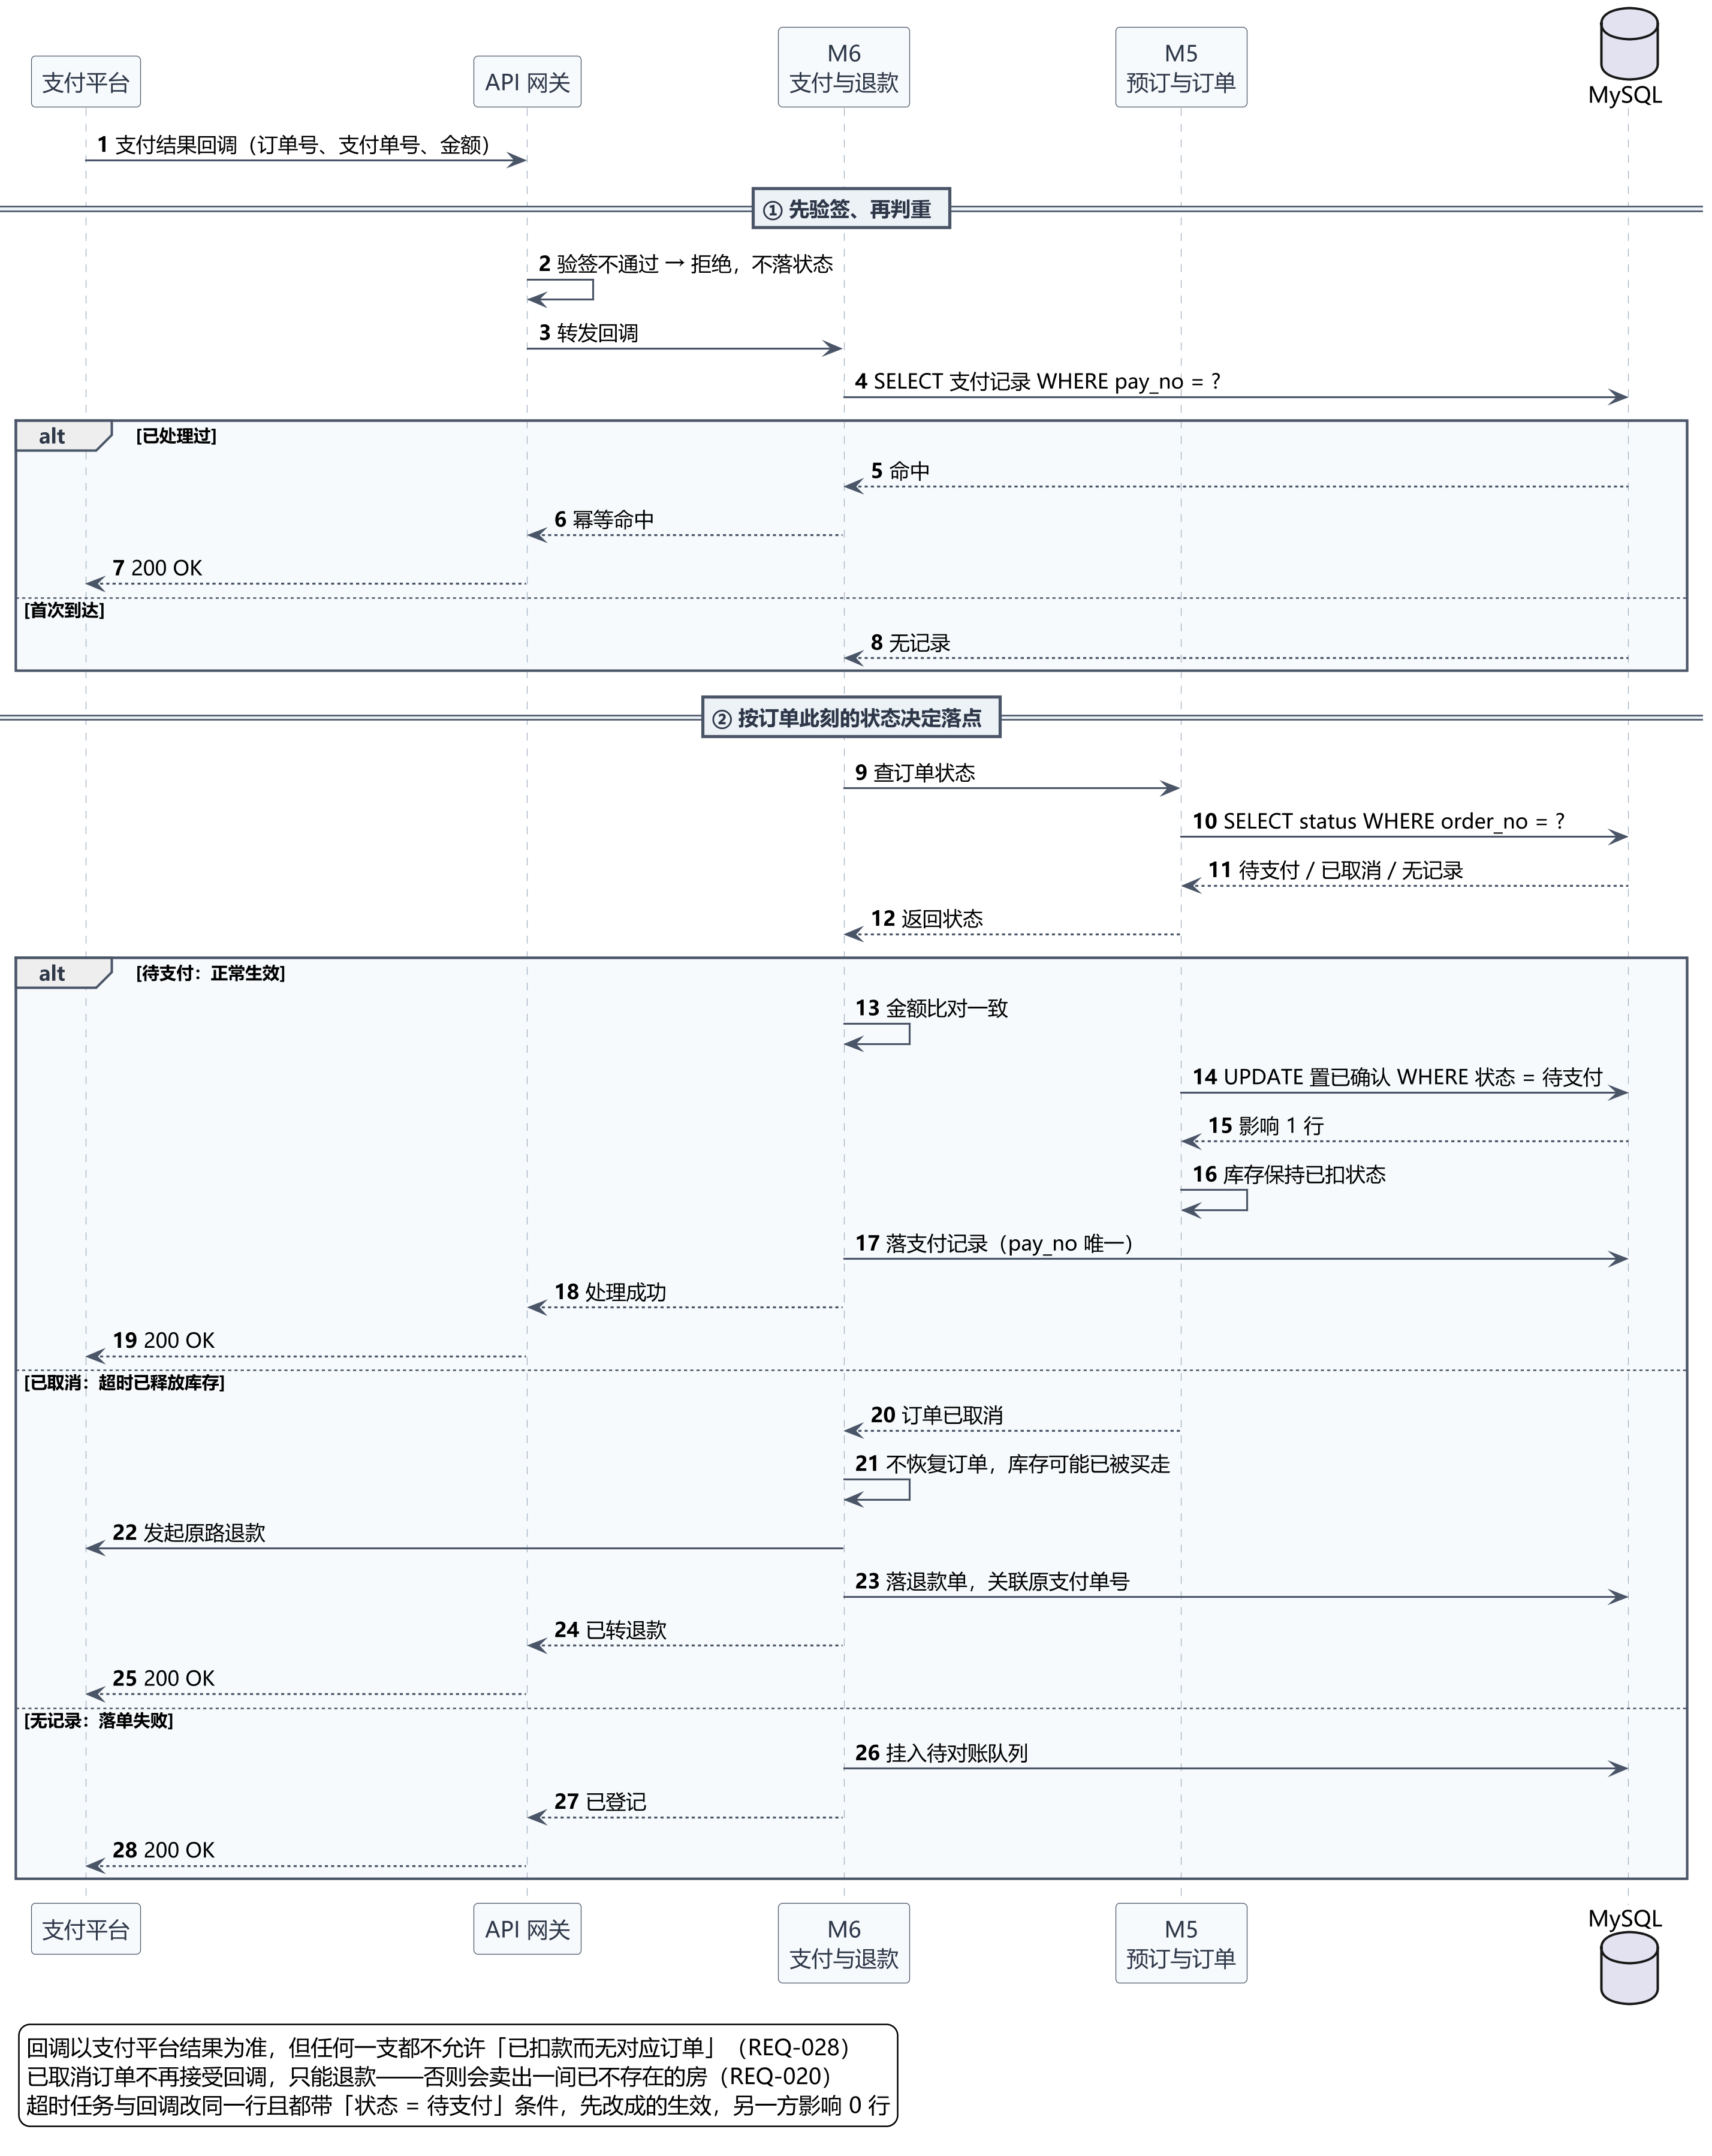
\includegraphics[width=0.77\textwidth]{../UML/UML时序图_支付回调.png}
\caption{UML 时序图：支付回调的三种落点}
\label{fig:seq3}
\end{figure}

支付回调这张图有一个 alt 三分支，分别对应订单此刻的三种状态：

\begin{itemize}
  \item \textbf{待支付}：正常生效，条件更新为已确认，落支付记录，库存保持已扣状态。
  \item \textbf{已取消}：说明超时任务先动手了，库存已经释放给别人。此时\textbf{不恢复订单}，改为原路退款——否则会卖出一间已经不存在的房。
  \item \textbf{无记录}：订单根本没建成功，挂入待对账队列，由每日对账补单或退款。
\end{itemize}

三种落点加起来，保证「已扣款而无对应订单」这个状态在任何时刻都不会停留超过一天。

\begin{figure}[htbp]
\centering
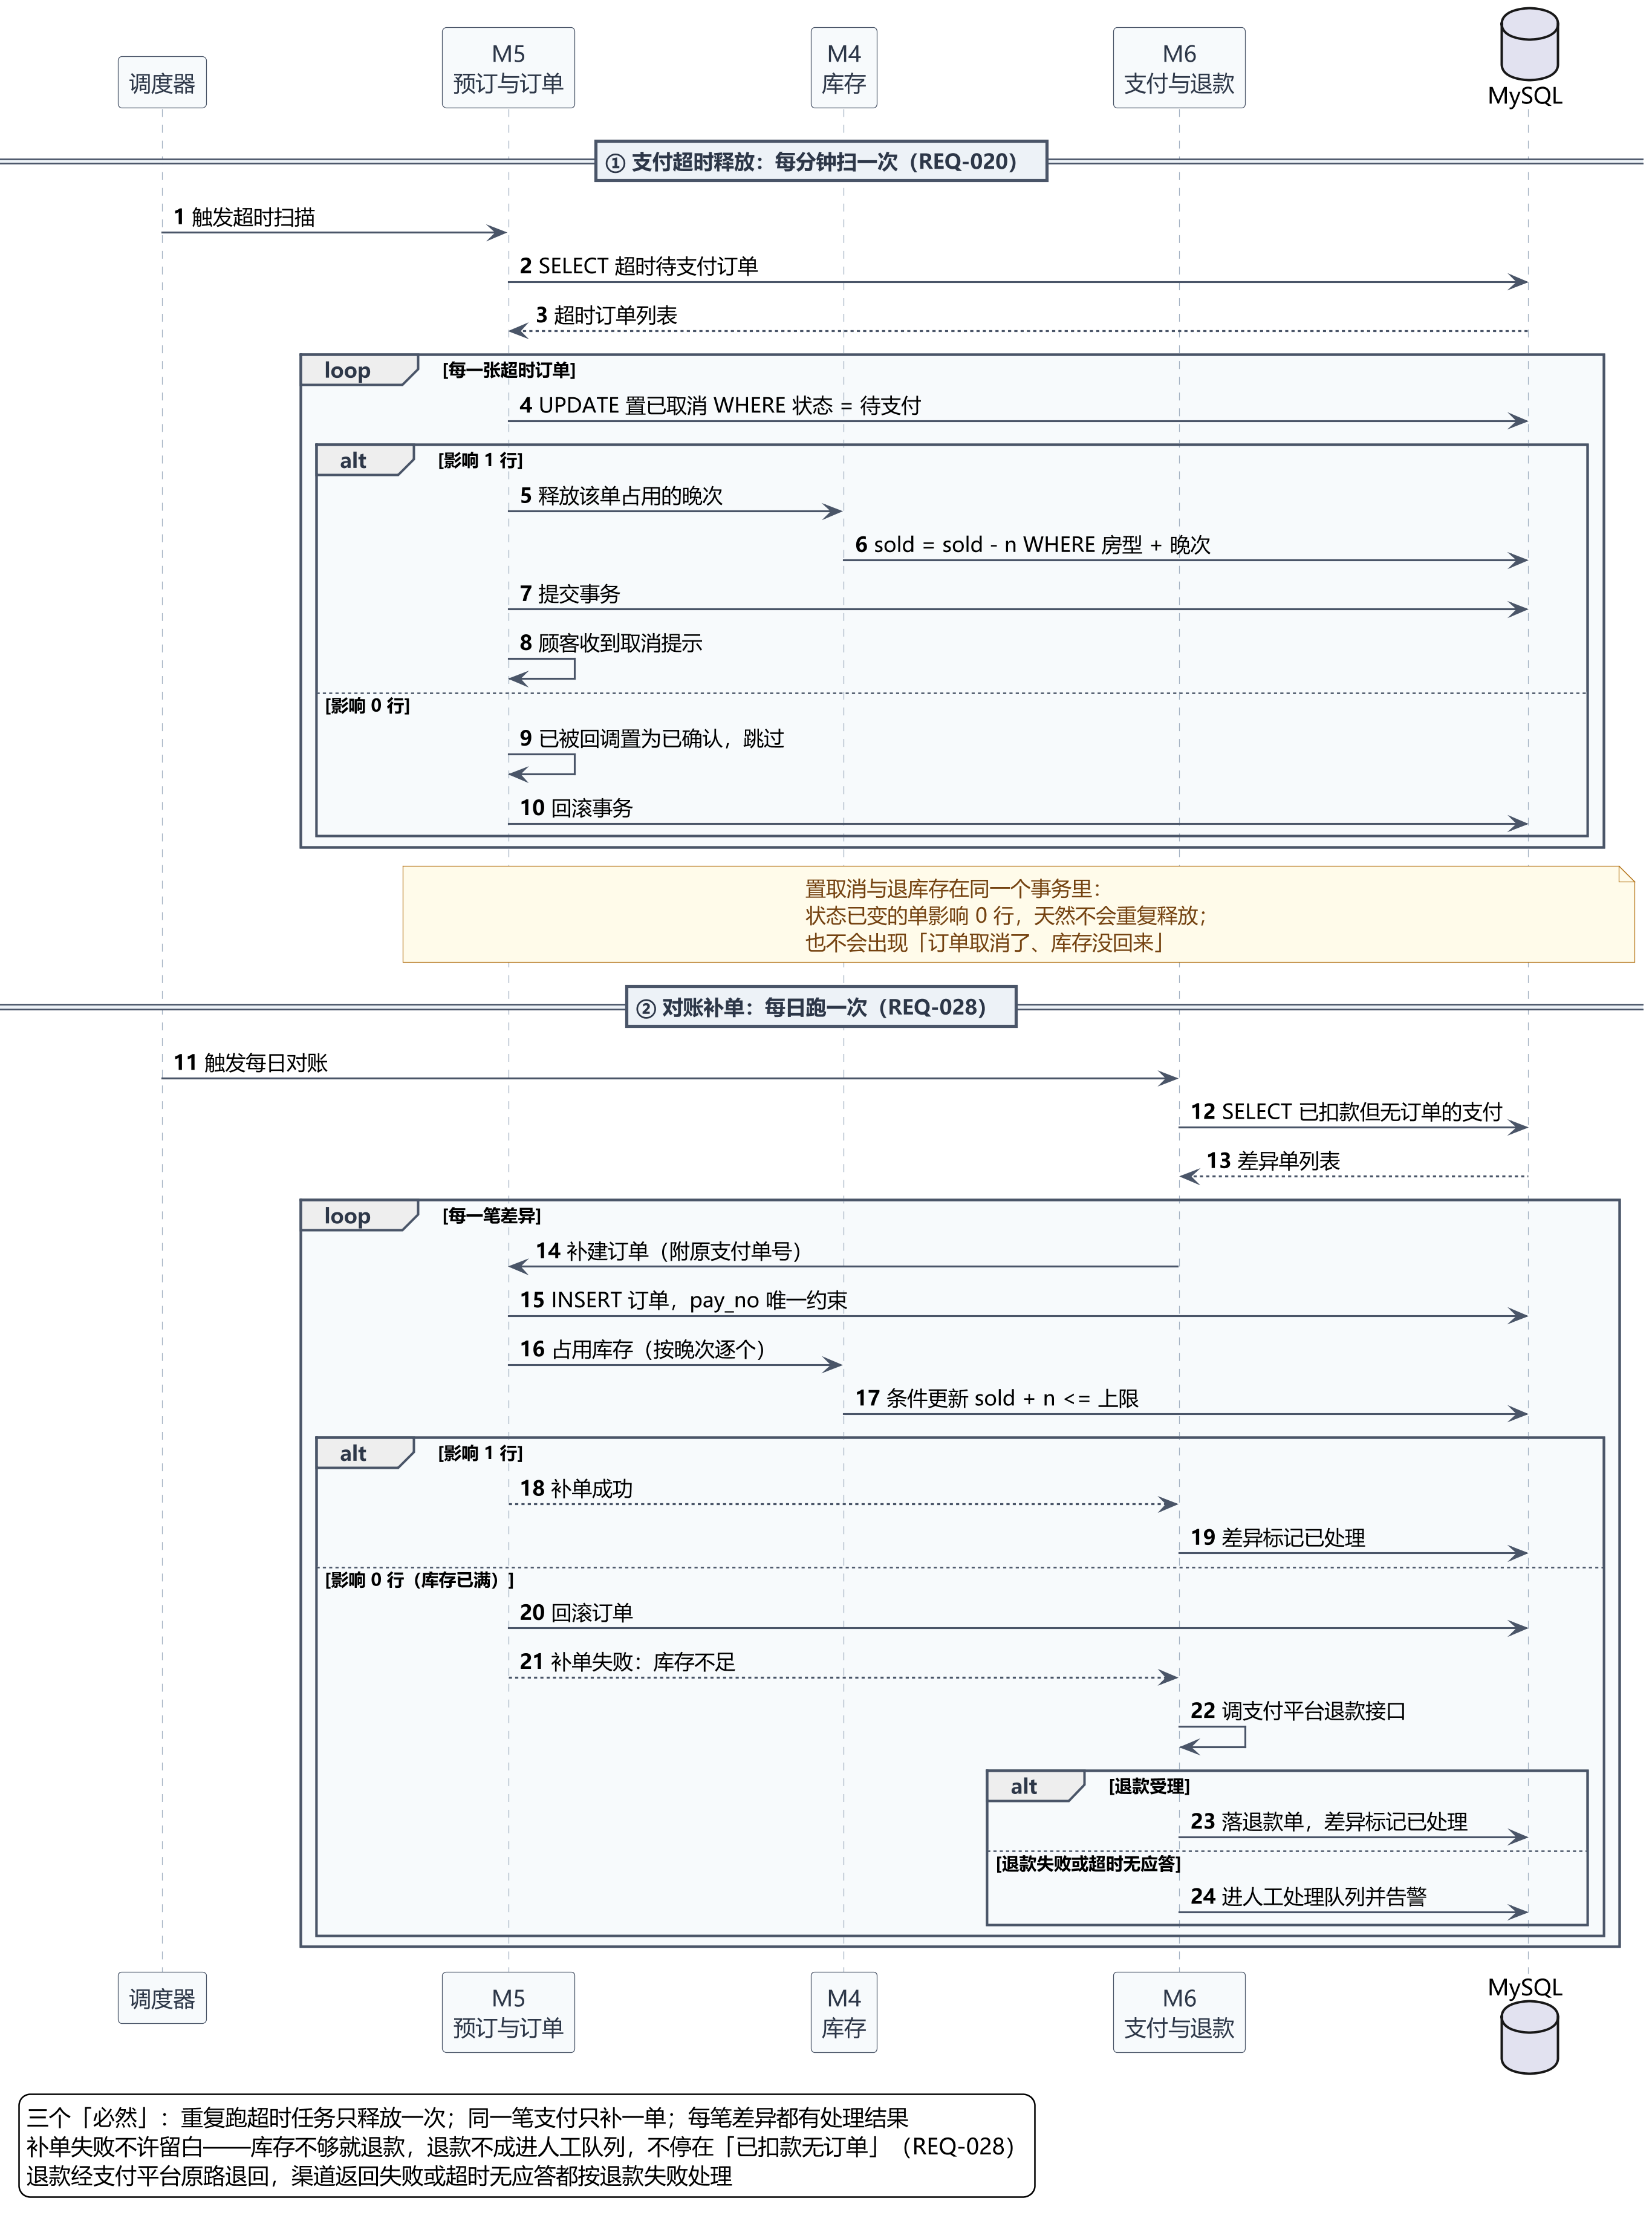
\includegraphics[width=0.72\textwidth]{../UML/UML时序图_超时释放与对账.png}
\caption{UML 时序图：超时释放与每日对账}
\label{fig:seq4}
\end{figure}

最后这张图有两条链路。上半部分是支付超时释放，每分钟扫描一次；关键在「置取消与退库存在同一个事务里」，并且置取消带「状态 = 待支付」条件——重复执行时影响 0 行，天然不会重复释放。

下半部分是对账补单，每日运行一次。补单逻辑里有一个必须写清的兜底：\textbf{库存不足时不是放弃，而是退款}。退款再失败就进人工队列并告警。这条兜底的意义是：对账的终点必须是「每笔差异都有处理结果」，不能停在「已扣款、无订单、待处理」。

% ==================== 六、UI 设计 ====================
\section{UI 设计}

顾客端采用手机画幅，前台、店长和平台端采用桌面画幅。19 屏的初稿由 AI 辅助生成 HTML 与 CSS，导入 Pixso 后调整部分界面并导出 PNG；设计分工与修改过程见第 7 章。

\subsection{界面一致性约束}

\subsubsection{状态标识}

四端使用同一套房态和订单状态色，颜色与文字标签同时标示状态。

{\tabfont
\begin{xltabular}{\textwidth}{@{}L{3.5cm}L{3.3cm}X@{}}
\caption{房态与订单状态的用色约定}\label{tab:state_color}\\
\toprule
状态 & 颜色 & 用途 \\
\midrule
\endfirsthead
\toprule
状态 & 颜色 & 用途 \\
\midrule
\endhead
\midrule
\multicolumn{3}{r}{\zihao{6}续下页}\\
\endfoot
\bottomrule
\endlastfoot
房间·空闲 & 绿（实线） & 可售 \\
房间·已预定 & 蓝（虚线） & 等待入住 \\
房间·已入住 & 品牌蓝（填充） & 在住 \\
房间·需打扫 & 橙 & 待处理 \\
房间·维修中 & 红 & 暂停销售 \\
房间·已退房 & 灰 & 待进入下一环节 \\
订单·待支付 & 橙 & 显示支付倒计时 \\
订单·已确认/已入住 & 蓝/品牌蓝 & 正常流程 \\
订单·已退房 & 灰 & 已完成 \\
订单·已取消/未到店 & 红 & 异常或终止 \\
\end{xltabular}
}


\subsubsection{示例数据}

界面示例统一采用 2026 年 10 月 31 日 13:47 的数据。08、11、12、13 屏分别展示房态、库存、价格和审批时，沿用第 1 章的 48 间房、维修 2 间及高级大床房线上余量 4 间等基准。

\subsection{顾客端（7 屏，手机 H5）}

顾客端按搜索、选房、下单、支付、查单和评价组织，底部提供首页、订单和我的三个入口。

\begin{figure}[htbp]
\centering
\begin{subfigure}[b]{0.31\textwidth}
  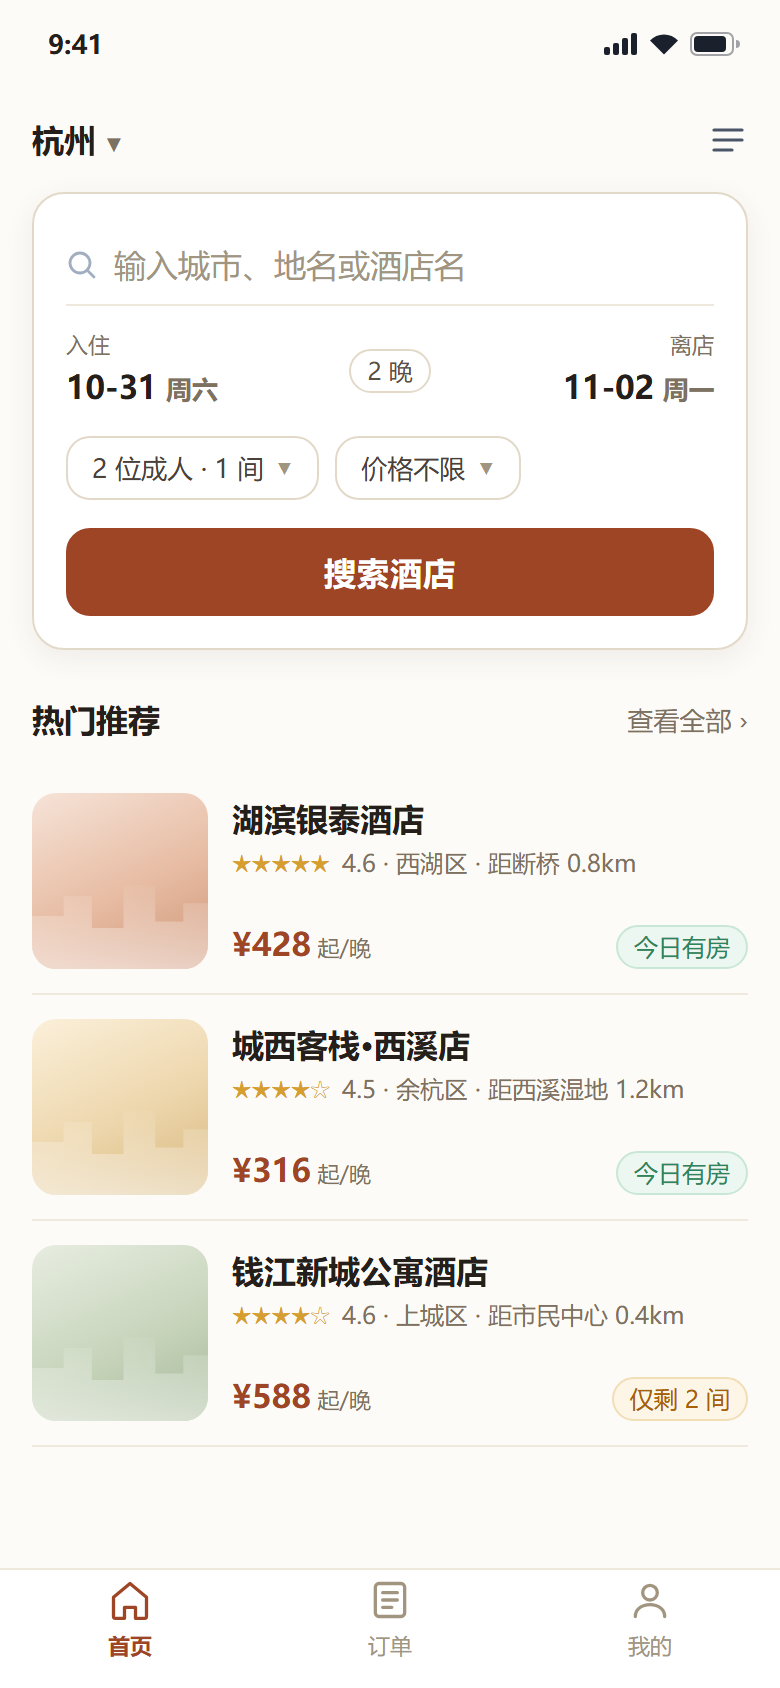
\includegraphics[width=\textwidth]{../UI界面/01_home_search.png}
  \caption{首页与搜索}
\end{subfigure}\hfill
\begin{subfigure}[b]{0.31\textwidth}
  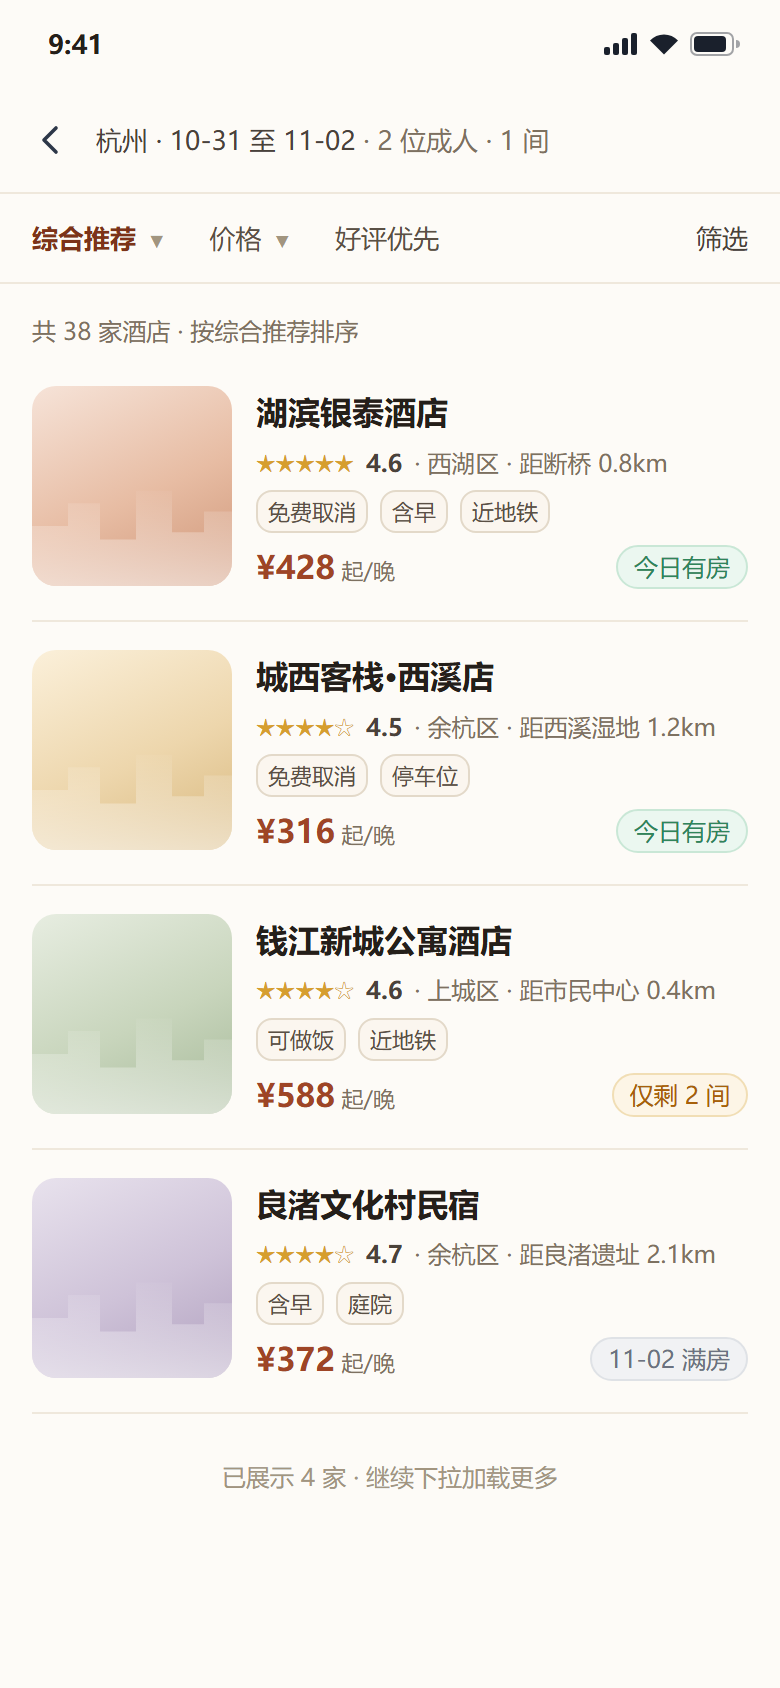
\includegraphics[width=\textwidth]{../UI界面/02_search_result.png}
  \caption{搜索结果}
\end{subfigure}\hfill
\begin{subfigure}[b]{0.31\textwidth}
  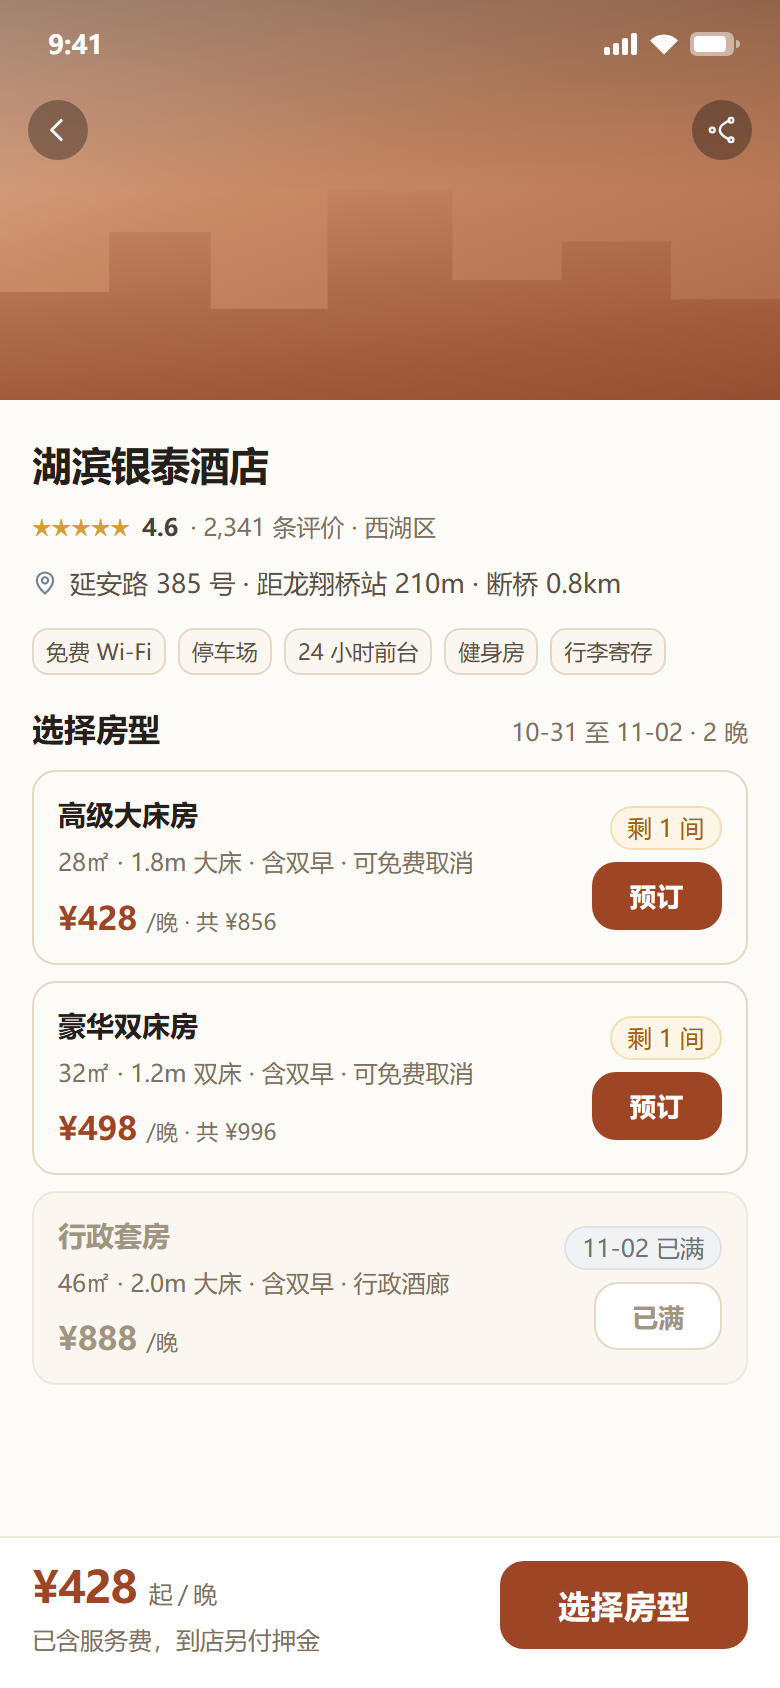
\includegraphics[width=\textwidth]{../UI界面/03_hotel_detail.png}
  \caption{酒店详情与房型}
\end{subfigure}
\caption{顾客端：搜索链路（01--03）}
\label{fig:ui_c1}
\end{figure}

\textbf{01 首页与搜索。} 展示城市、入住日期、离店日期、人数和价格条件，下方推荐门店并显示房量概况。房型的逐晚余量在详情页核对（REQ-002、REQ-013）。

\textbf{02 搜索结果。} 展示当前查询条件、排序筛选项及门店卡片；满房提示写明对应日期，避免将某一晚售罄误写成整店售罄（REQ-013）。

\textbf{03 酒店详情与房型选择。} 房型列表展示单价、总价和所选住期的可订量。示例包括：

\begin{itemize}
  \item 高级大床房 ¥428/晚 · 共 ¥856 · \textbf{剩 1 间}，可预订；
  \item 豪华双床房 ¥498/晚 · 共 ¥996 · \textbf{剩 1 间}，可预订；
  \item 行政套房 ¥888/晚 · \textbf{11-02 已满}，按钮置灰标注「已满」。
\end{itemize}

多晚可订量取各晚余量的最小值；行政套房有一晚售罄，因此不可提交两晚预订（REQ-013）。

\begin{figure}[htbp]
\centering
\begin{subfigure}[b]{0.31\textwidth}
  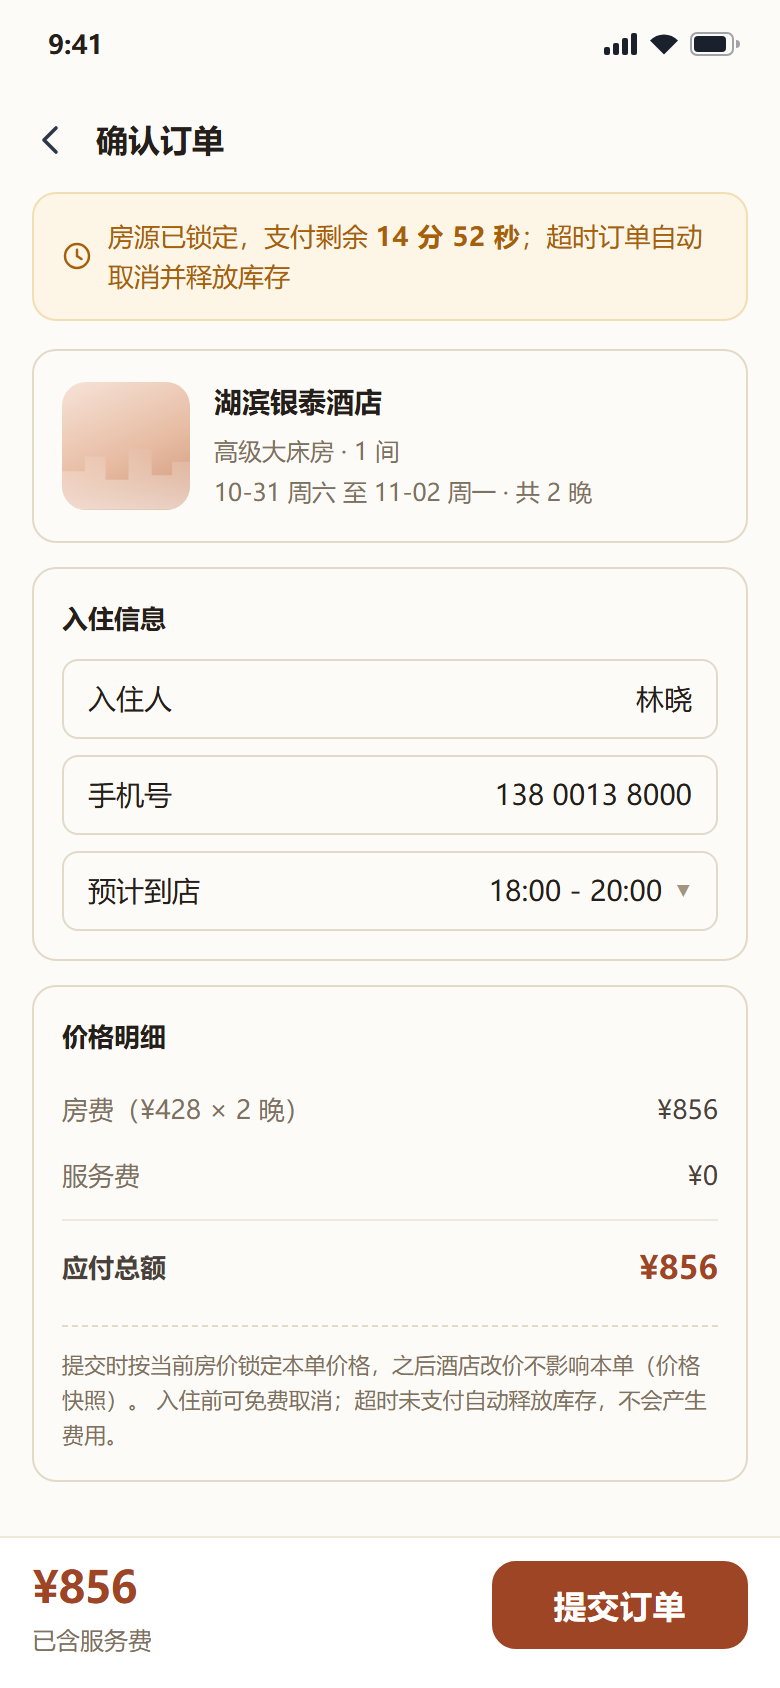
\includegraphics[width=\textwidth]{../UI界面/04_order_confirm.png}
  \caption{订单确认}
\end{subfigure}\hfill
\begin{subfigure}[b]{0.31\textwidth}
  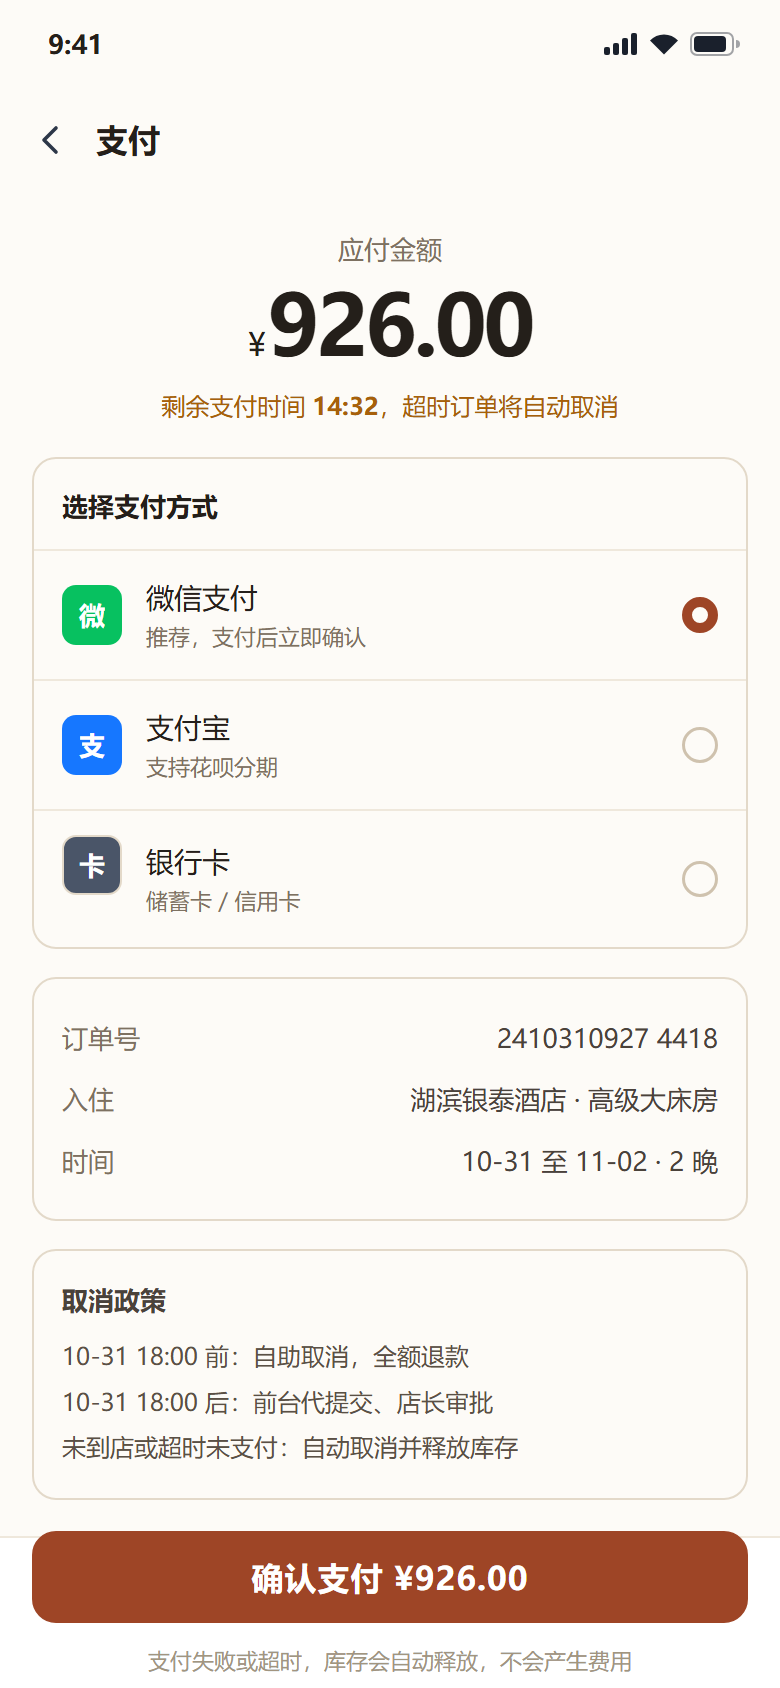
\includegraphics[width=\textwidth]{../UI界面/05_payment.png}
  \caption{支付}
\end{subfigure}\hfill
\begin{subfigure}[b]{0.31\textwidth}
  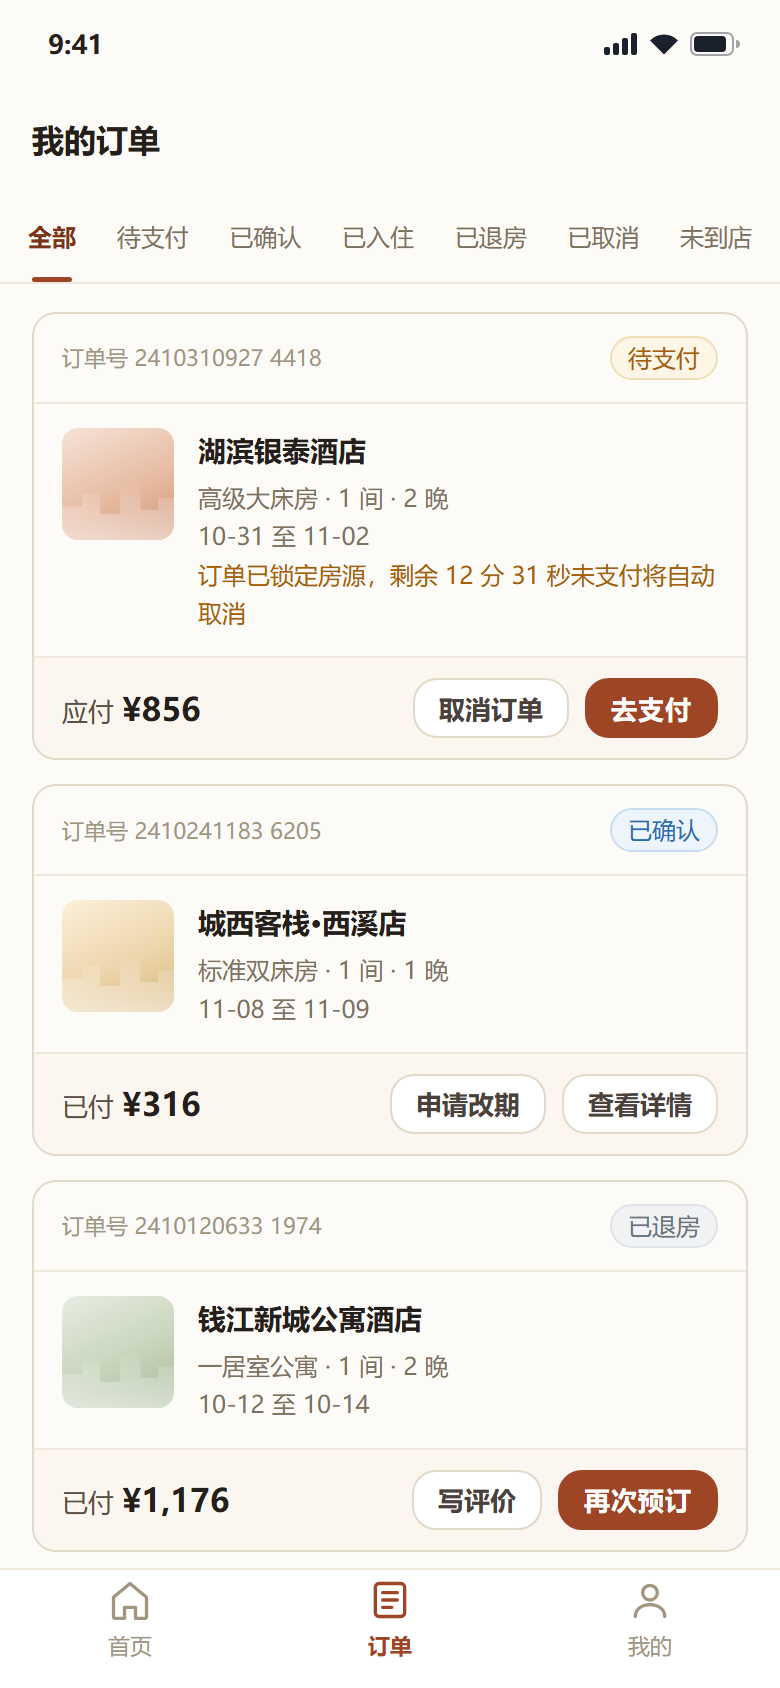
\includegraphics[width=\textwidth]{../UI界面/06_my_orders.png}
  \caption{我的订单}
\end{subfigure}
\caption{顾客端：确认、支付与订单（04--06）}
\label{fig:ui_c2}
\end{figure}

\textbf{04 订单确认。} 显示支付倒计时、入住人信息、价格明细和取消政策；超时未支付时取消订单并释放库存（REQ-020）。

示例订单为 ¥428 $\times$ 2 晚，共 ¥856；提交时将单价写入订单明细作为快照（REQ-023）。

\textbf{05 支付。} 展示应付金额、剩余支付时间、支付方式和取消政策：

\begin{itemize}
  \item 10-31 18:00 前：自助取消，全额退款（REQ-021 前段）；
  \item 10-31 18:00 后：前台代提交、店长审批（REQ-021 后段）；
  \item 未到店或超时未支付：自动取消并释放库存（REQ-020、REQ-022）。
\end{itemize}


\textbf{06 我的订单。} 支持按订单状态筛选。示例卡片提供以下操作：

\begin{itemize}
  \item 待支付：取消订单、去支付，并显示剩余支付时间；
  \item 已确认：申请改期、查看详情；
  \item 已退房：写评价、再次预订（REQ-003）。
\end{itemize}


\begin{figure}[htbp]
\centering
\begin{subfigure}[b]{0.34\textwidth}
  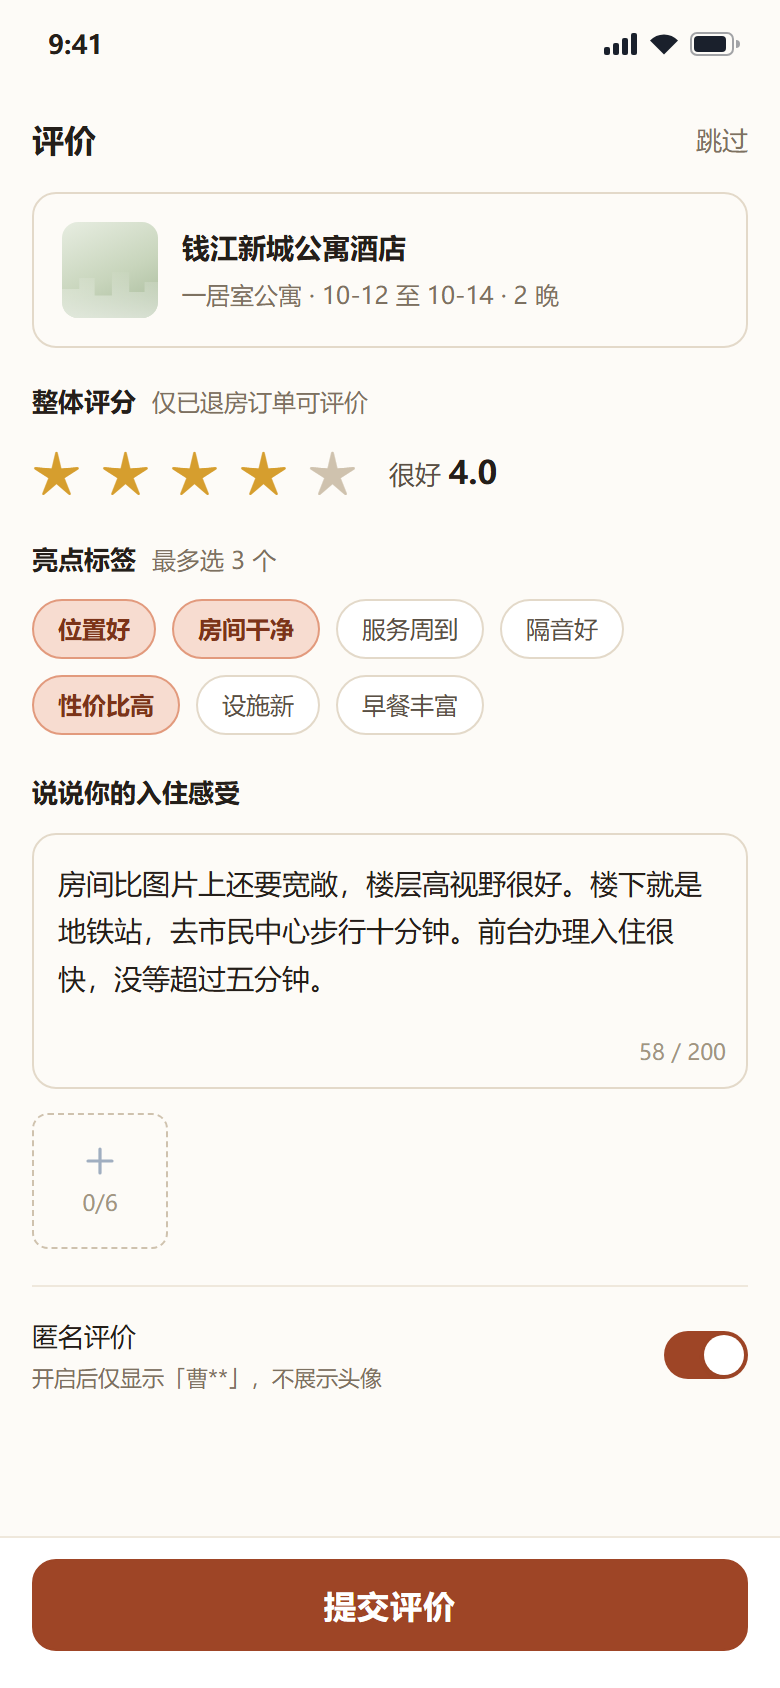
\includegraphics[width=\textwidth]{../UI界面/07_review_submit.png}
  \caption{评价提交}
\end{subfigure}
\caption{顾客端：评价提交（07）}
\label{fig:ui_c3}
\end{figure}

\textbf{07 评价提交。} 仅向已退房订单开放，包含评分、最多三个标签、200 字以内的文字和匿名选项（REQ-003）。

\subsection{前台端（4 屏，桌面工作台）}

前台端按房态、入住、退房和线下开单分为四屏。

\begin{figure}[htbp]
\centering
\begin{subfigure}[b]{0.95\textwidth}
  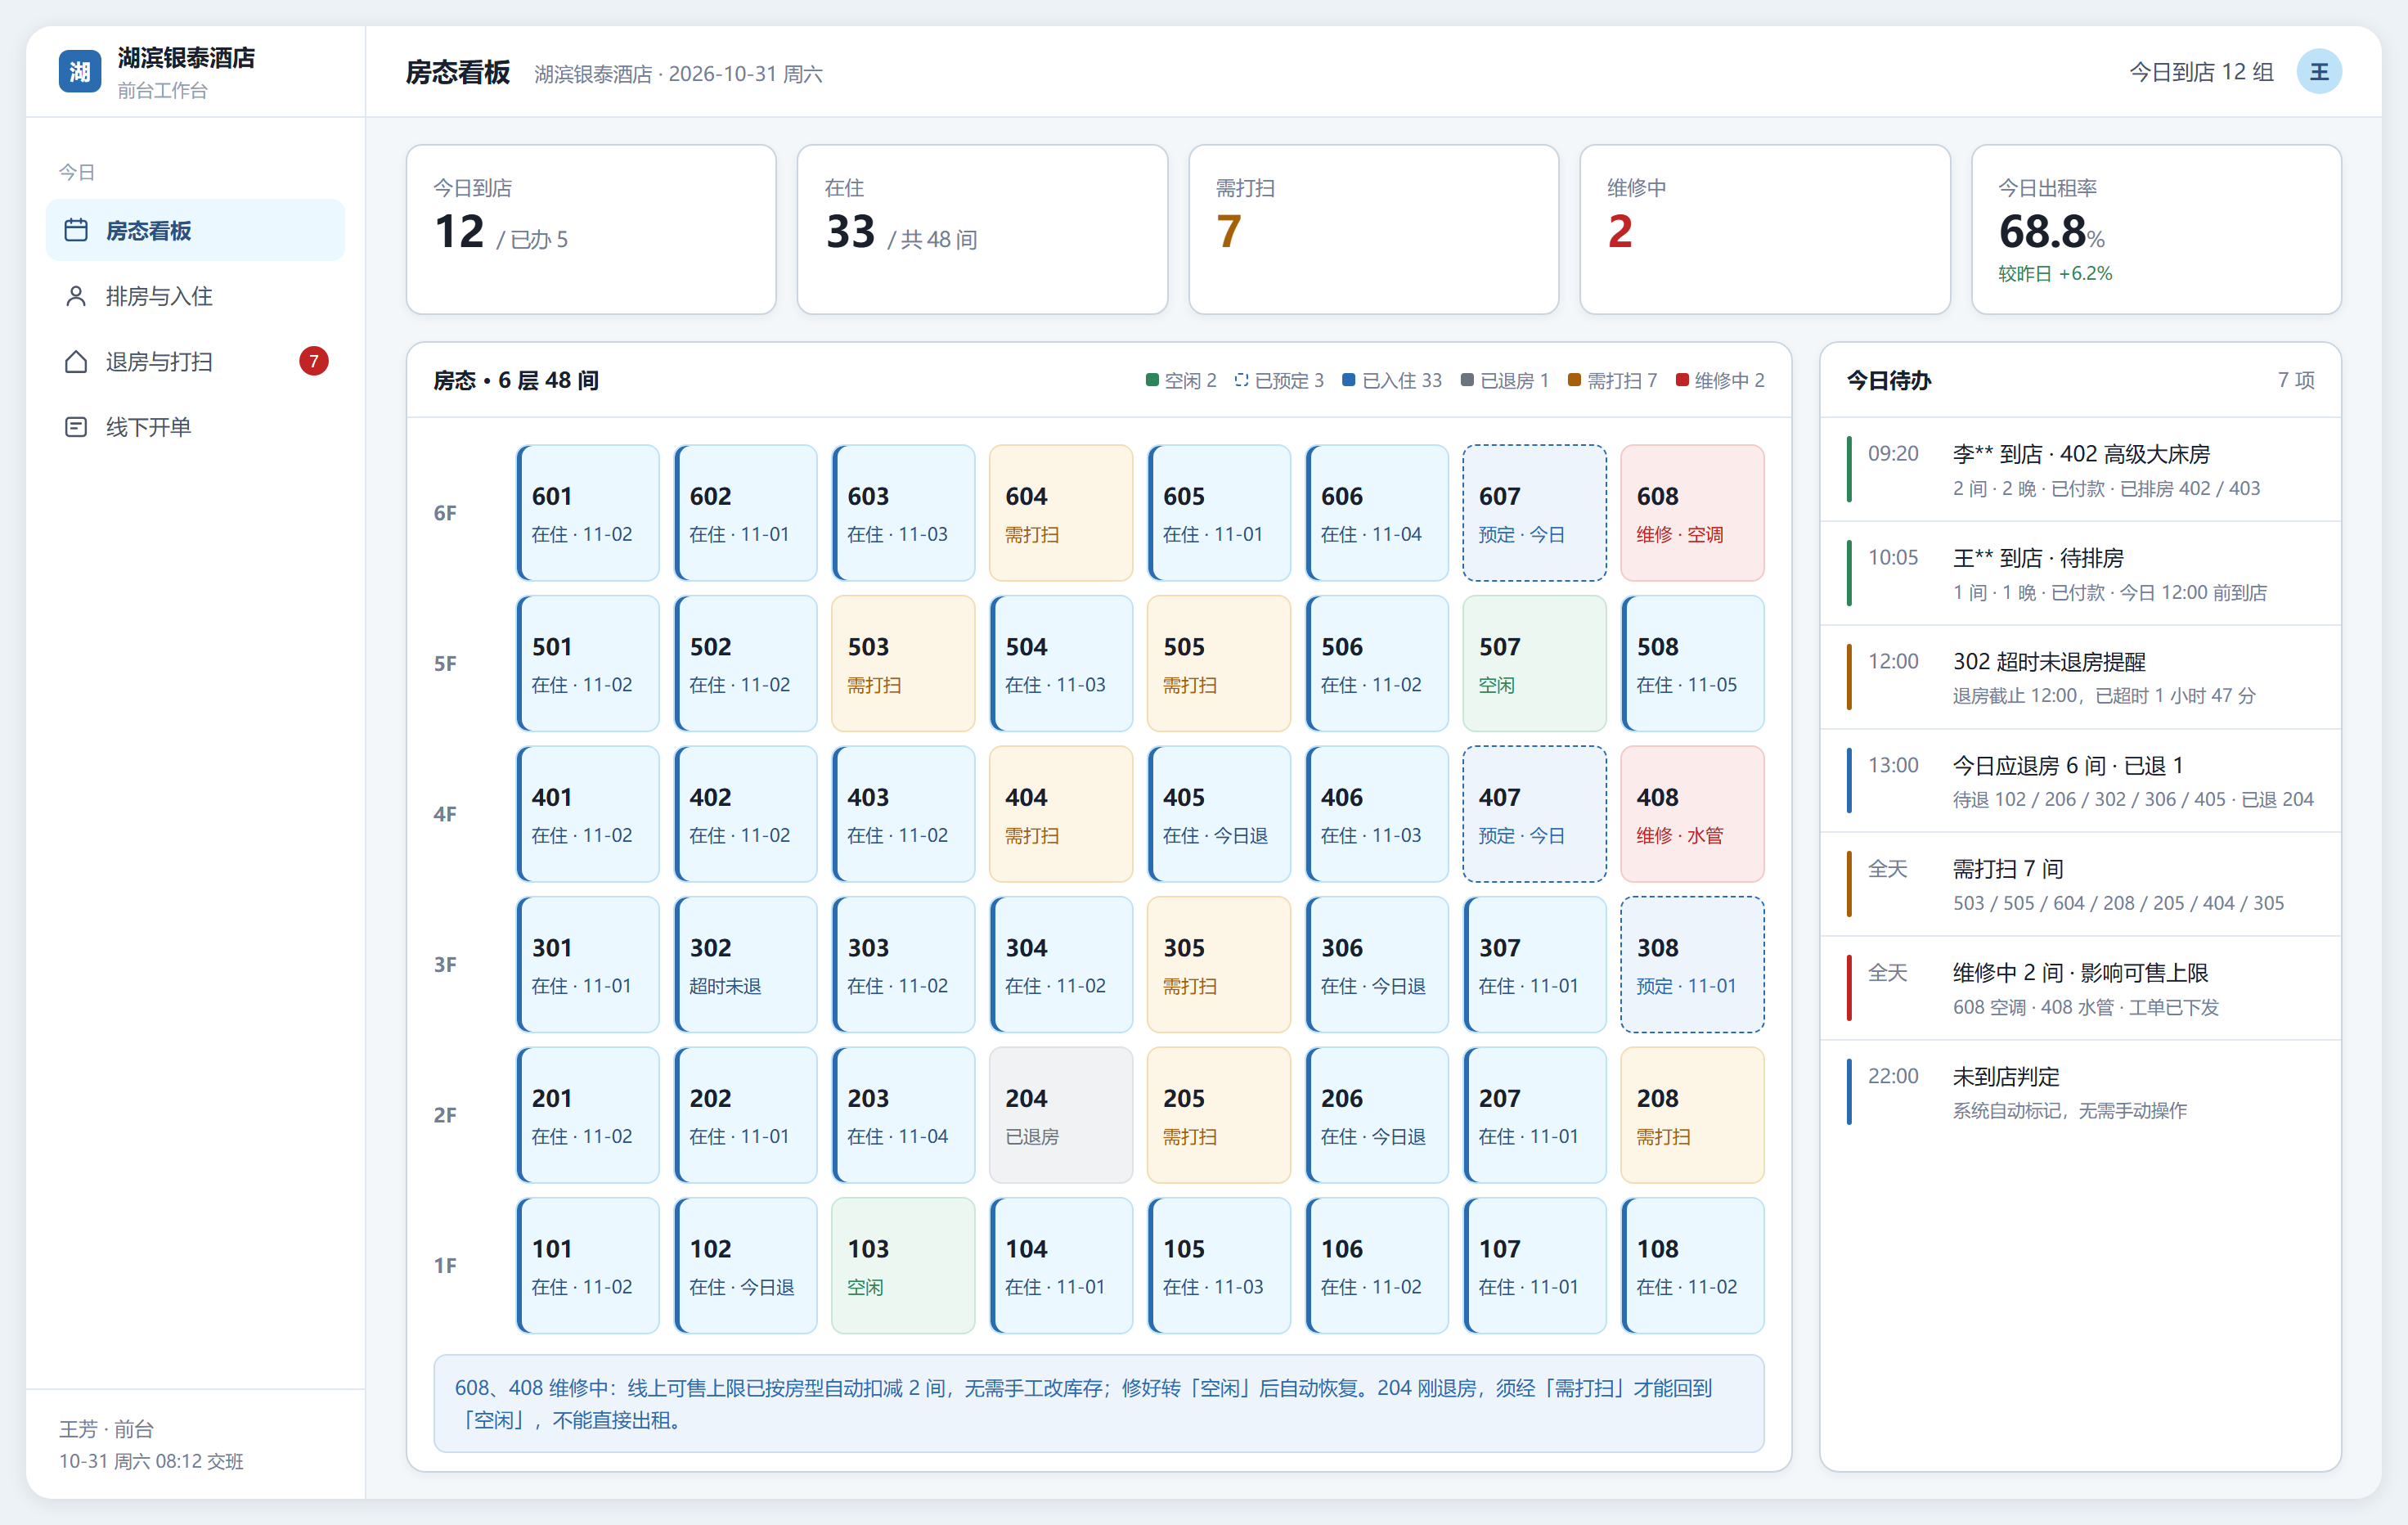
\includegraphics[width=\textwidth]{../UI界面/08_room_board.png}
  \caption{房态看板与今日待办}
\end{subfigure}\\[3pt]
\begin{subfigure}[b]{0.95\textwidth}
  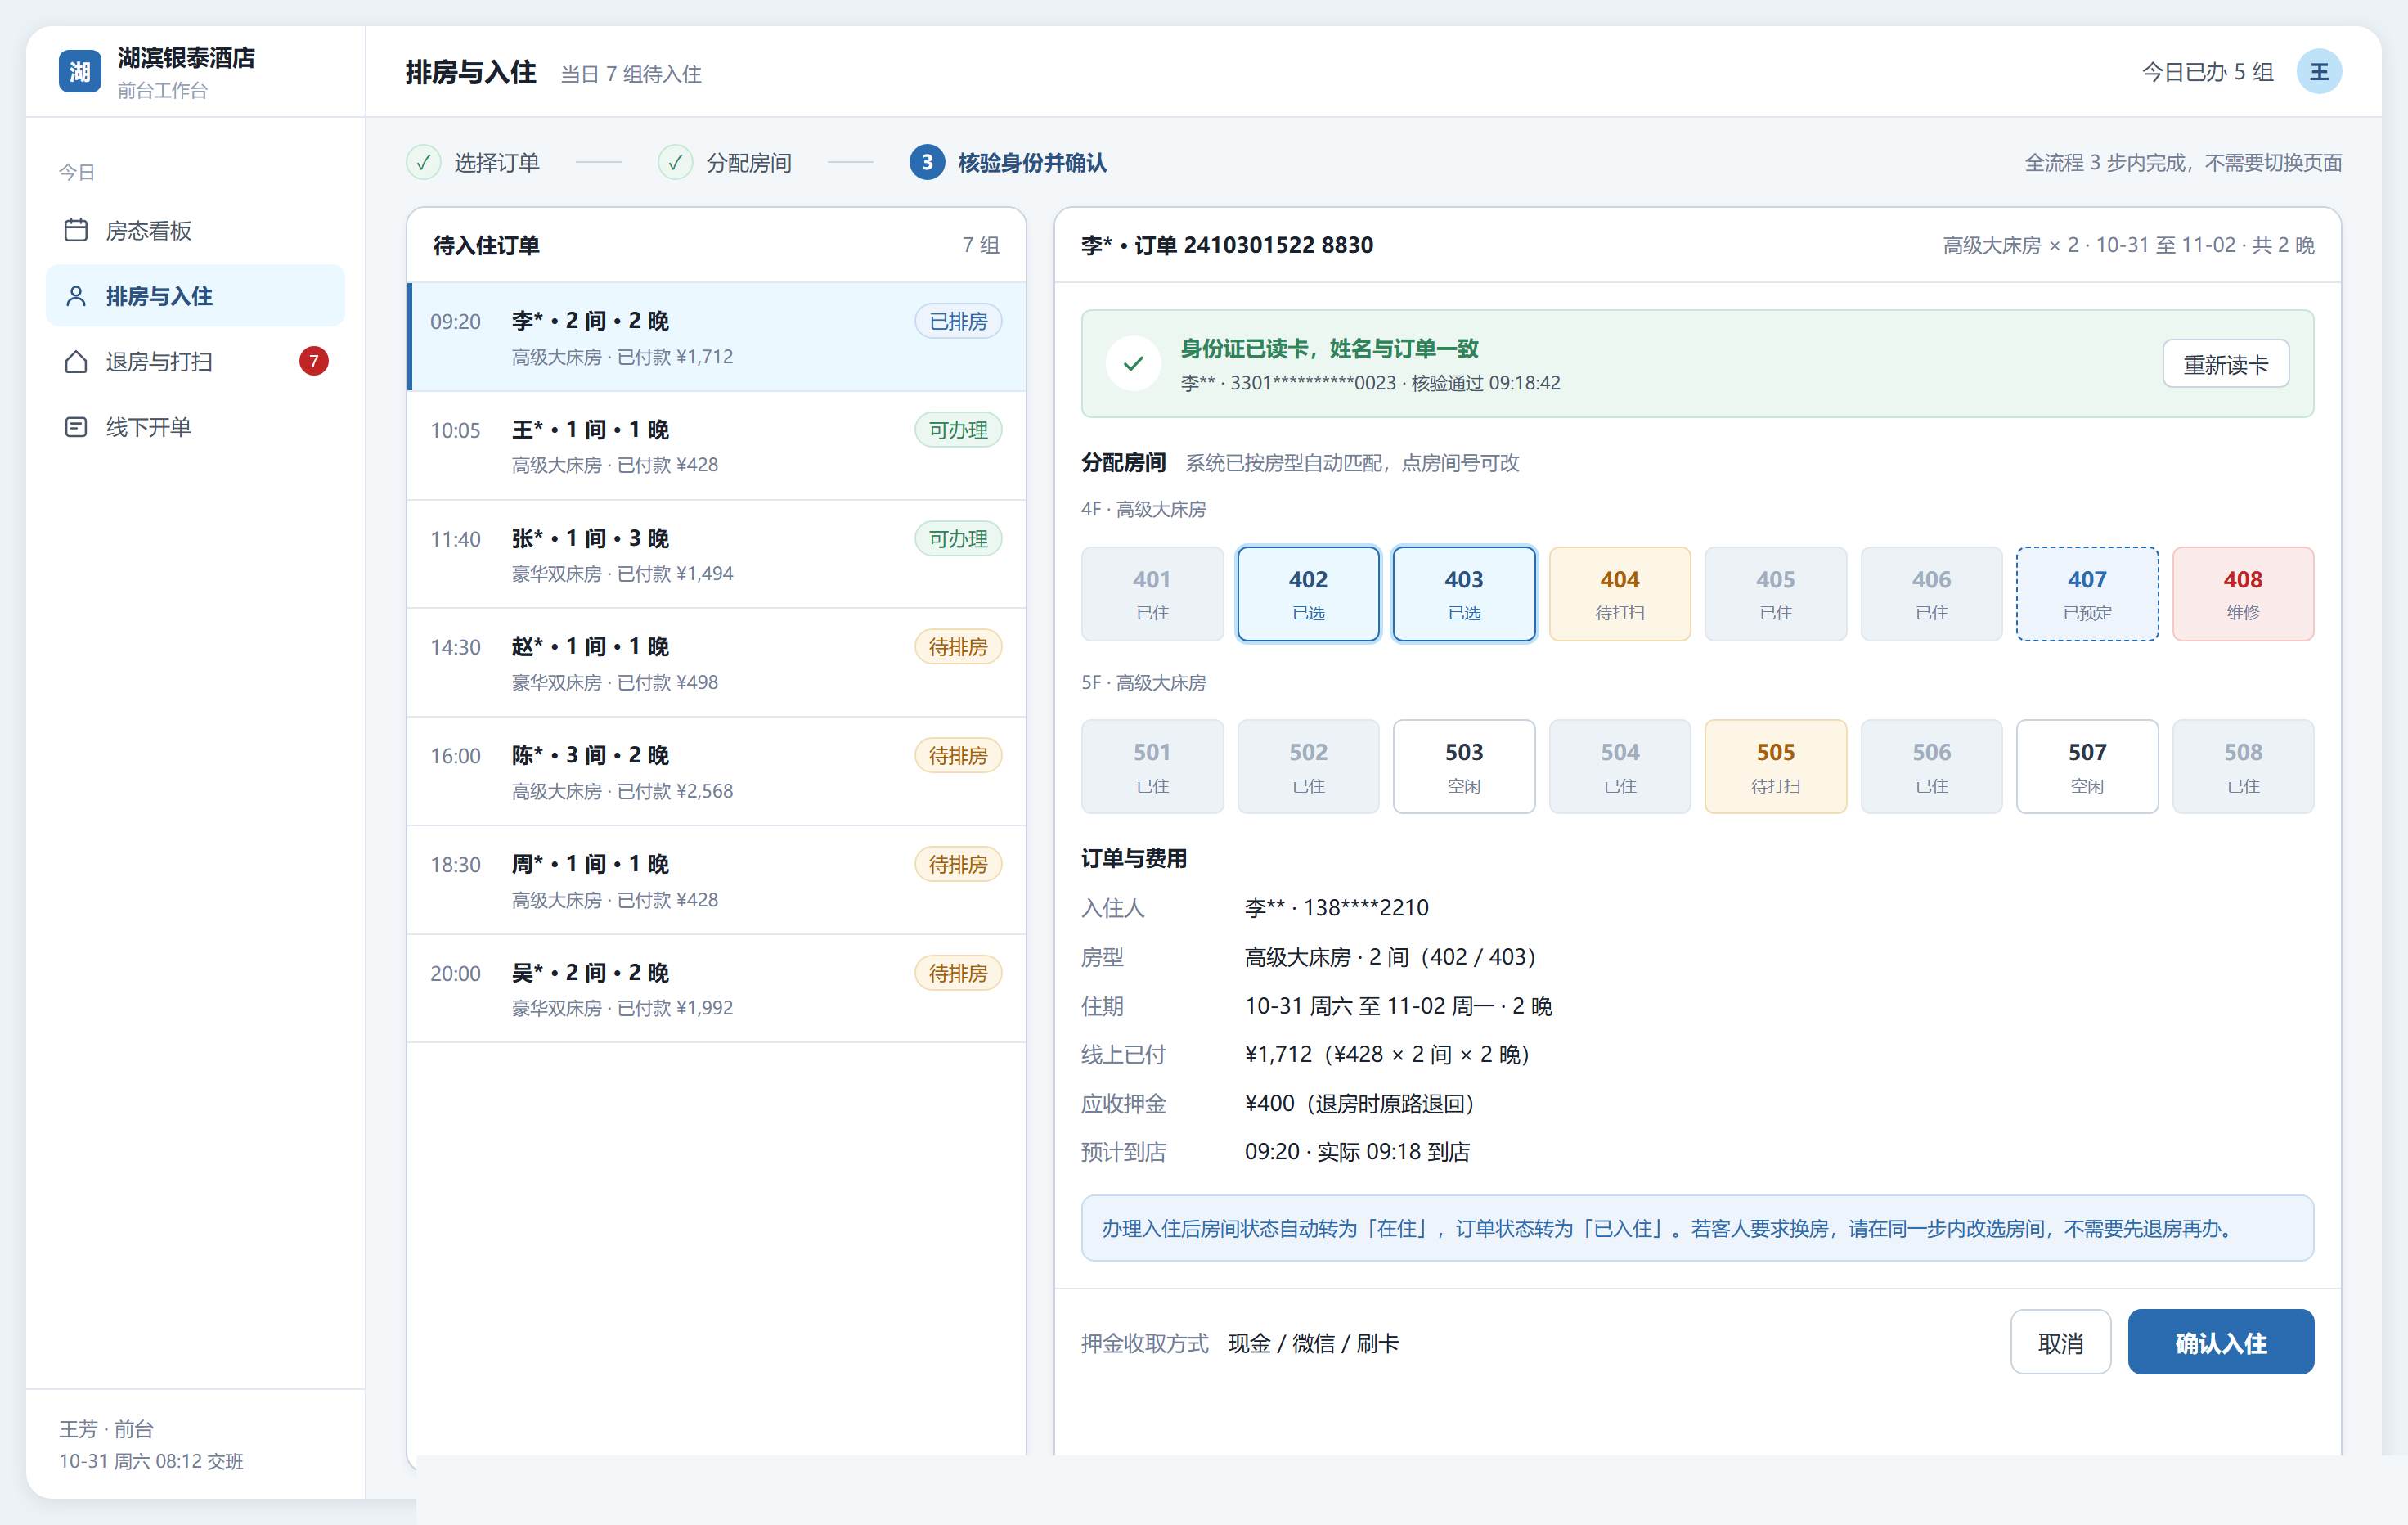
\includegraphics[width=\textwidth]{../UI界面/09_checkin.png}
  \caption{排房与入住办理}
\end{subfigure}
\caption{前台端：房态看板与入住（08--09）}
\label{fig:ui_f1}
\end{figure}

\textbf{08 房态看板。} 按楼层显示 48 间房的六种房态，并汇总在住 33 间、需打扫 7 间、维修中 2 间。超时未退和维修房间单独标示；维修数用于计算日库存上限（REQ-005、REQ-022、REQ-034）。

\textbf{09 排房与入住。} 依次选择订单、分配房间、核验身份并确认，控制在三步内（REQ-018）。系统提供建议房号，前台可改选；维修中、已入住、已预定及待打扫的房间不可选（REQ-024）。

\begin{figure}[htbp]
\centering
\begin{subfigure}[b]{0.95\textwidth}
  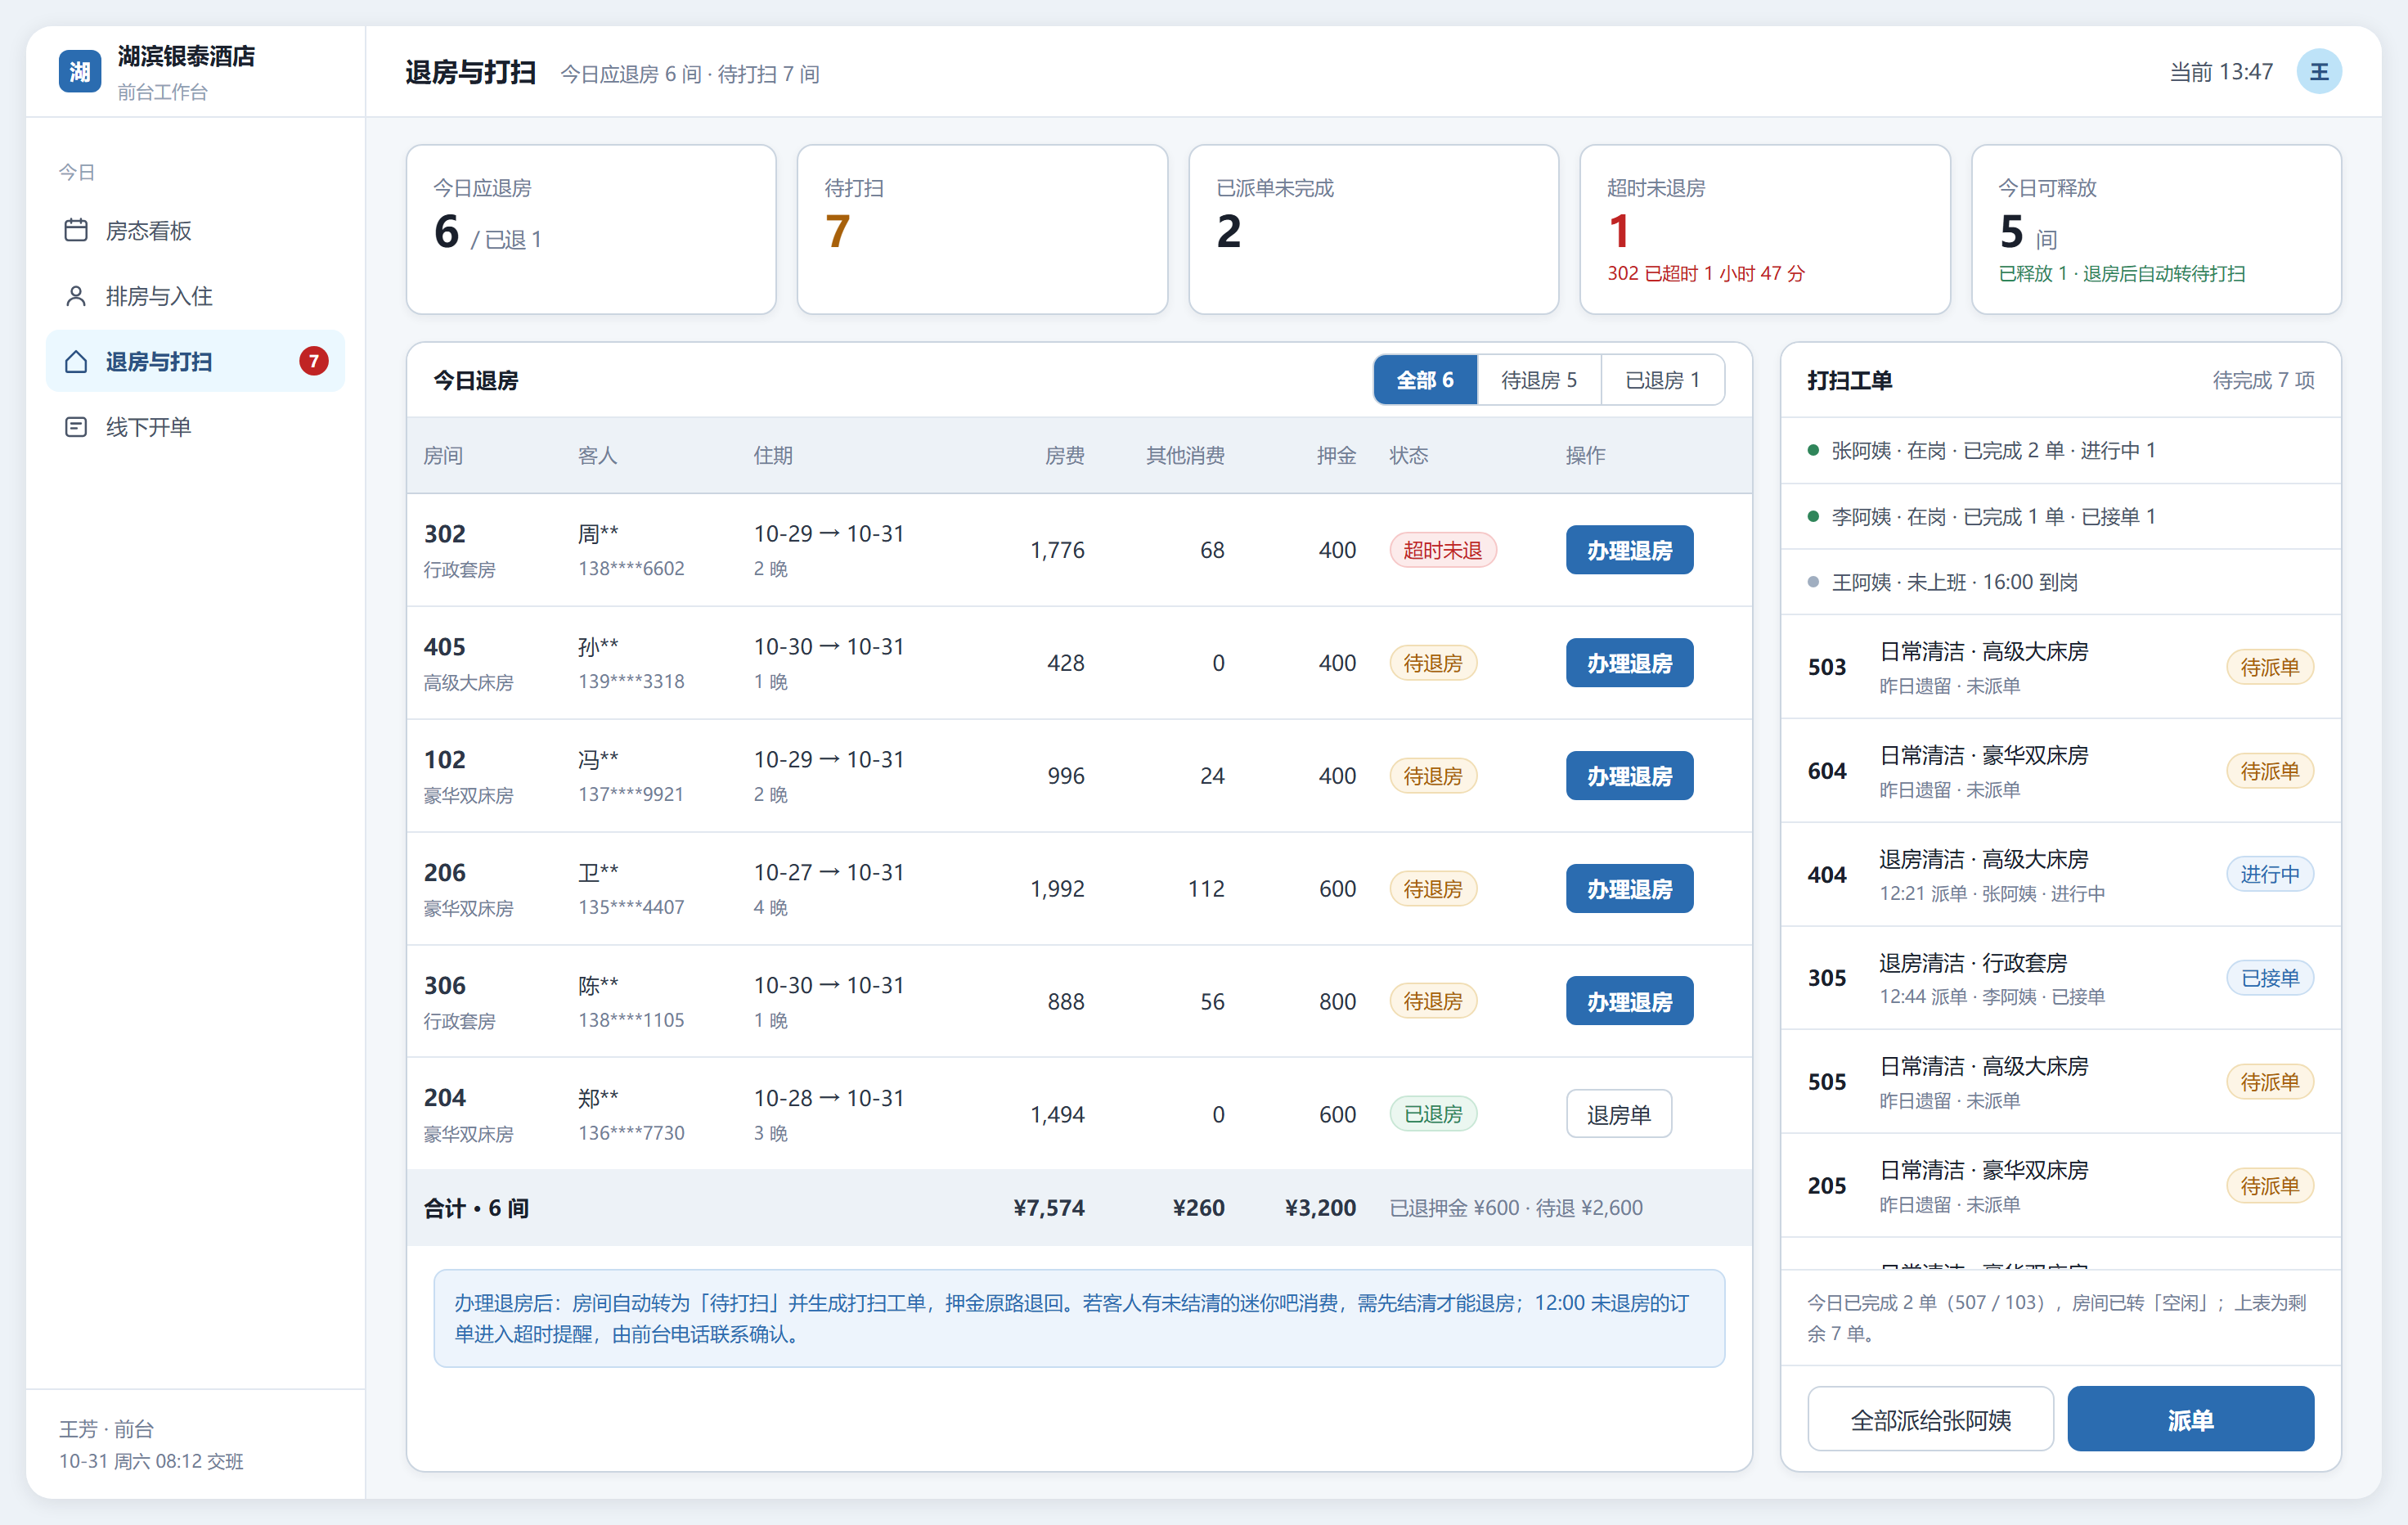
\includegraphics[width=\textwidth]{../UI界面/10_housekeeping.png}
  \caption{退房与打扫}
\end{subfigure}\\[3pt]
\begin{subfigure}[b]{0.95\textwidth}
  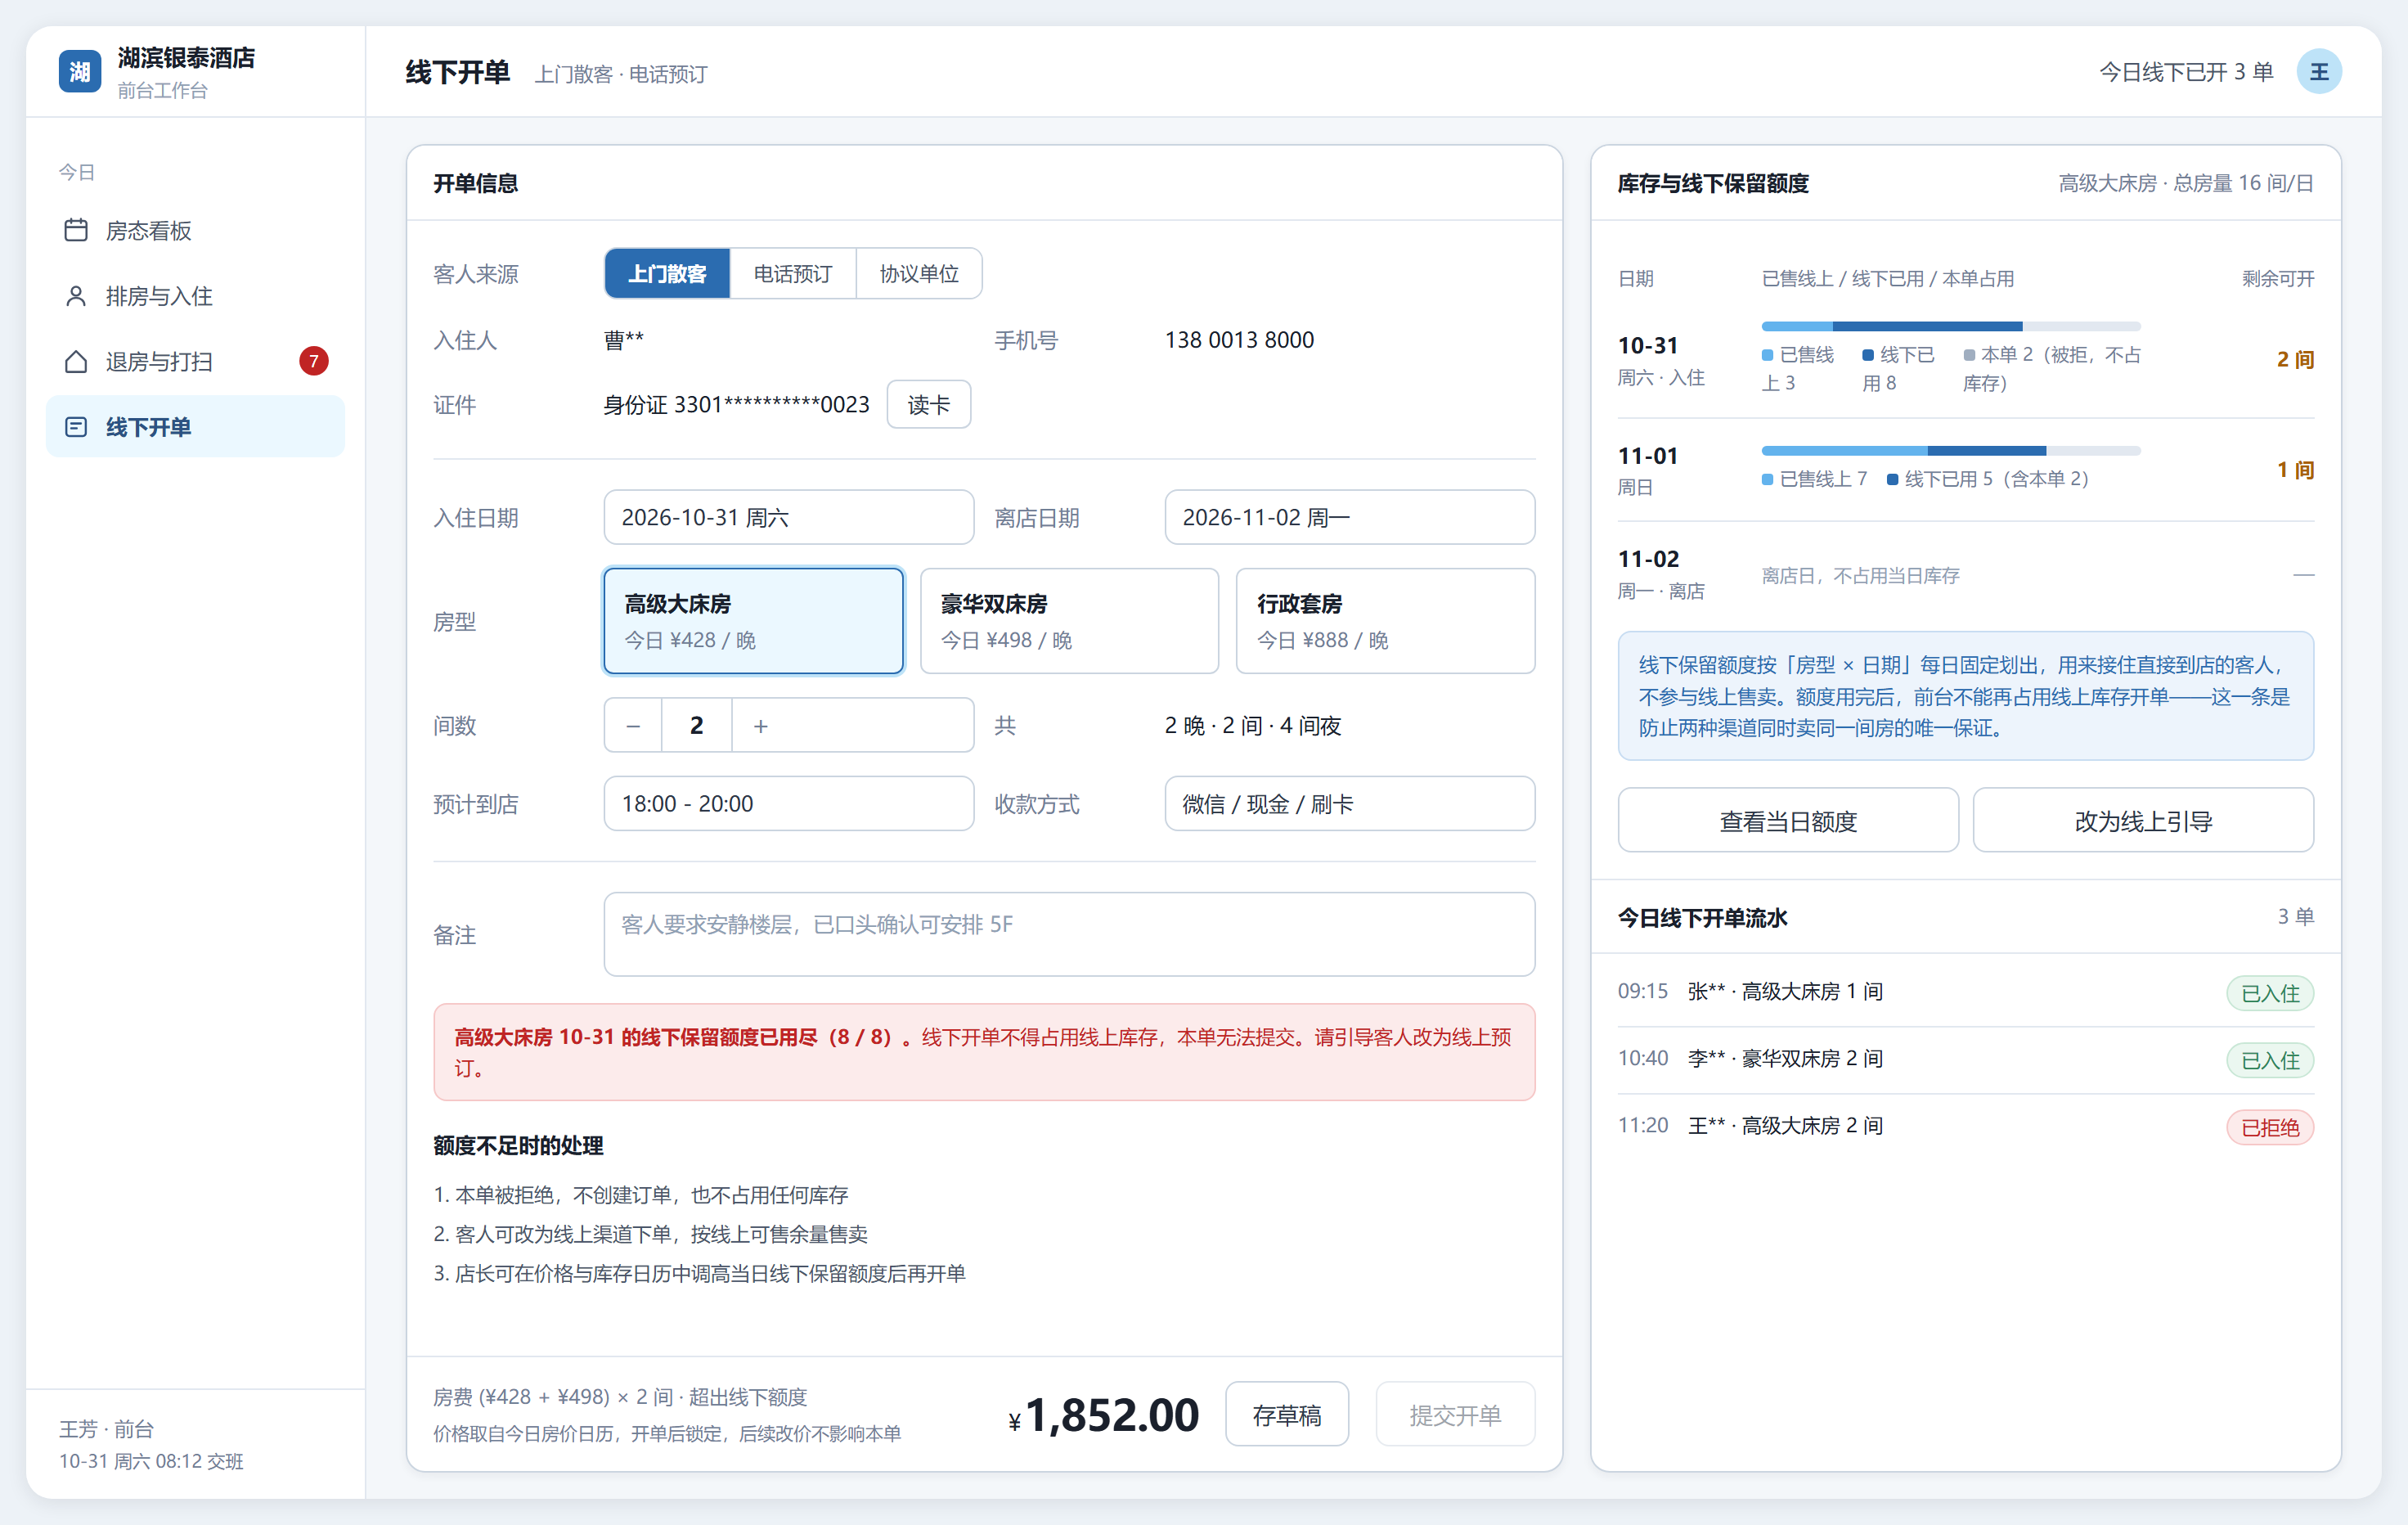
\includegraphics[width=\textwidth]{../UI界面/11_walkin_order.png}
  \caption{线下开单与库存校验}
\end{subfigure}
\caption{前台端：退房与线下开单（10--11）}
\label{fig:ui_f2}
\end{figure}

\textbf{10 退房与打扫。} 列出应退房、已退房、待打扫与超时未退房记录；每行可直接办理退房并派发打扫工单。房费、其他消费和押金分列，供退房结算使用（REQ-003、REQ-025）。

\textbf{11 线下开单。} 前台填写入住人、住期、房型、间数和收款方式；系统逐晚展示线上已售、线下已用和剩余可开量。线下保留额度不足时，界面提示：

\begin{quote}
\zihao{5}高级大床房 10-31 的线下保留额度已用尽（8 / 8）。继续开单将占用线上可售库存，可能造成线上超卖。请改为引导客人线上预订，或提交店长审批后再开单。
\end{quote}

超额开单提交后进入待审批状态，审批通过前不占库存；批准后重新校验并扣减库存，不足则开单失败。成功开单后生成排房任务（REQ-033）。

\subsection{店长端（4 屏，桌面后台）}

店长端提供定价、审批、排班评价和消息查询四项主要入口。

\begin{figure}[htbp]
\centering
\begin{subfigure}[b]{0.95\textwidth}
  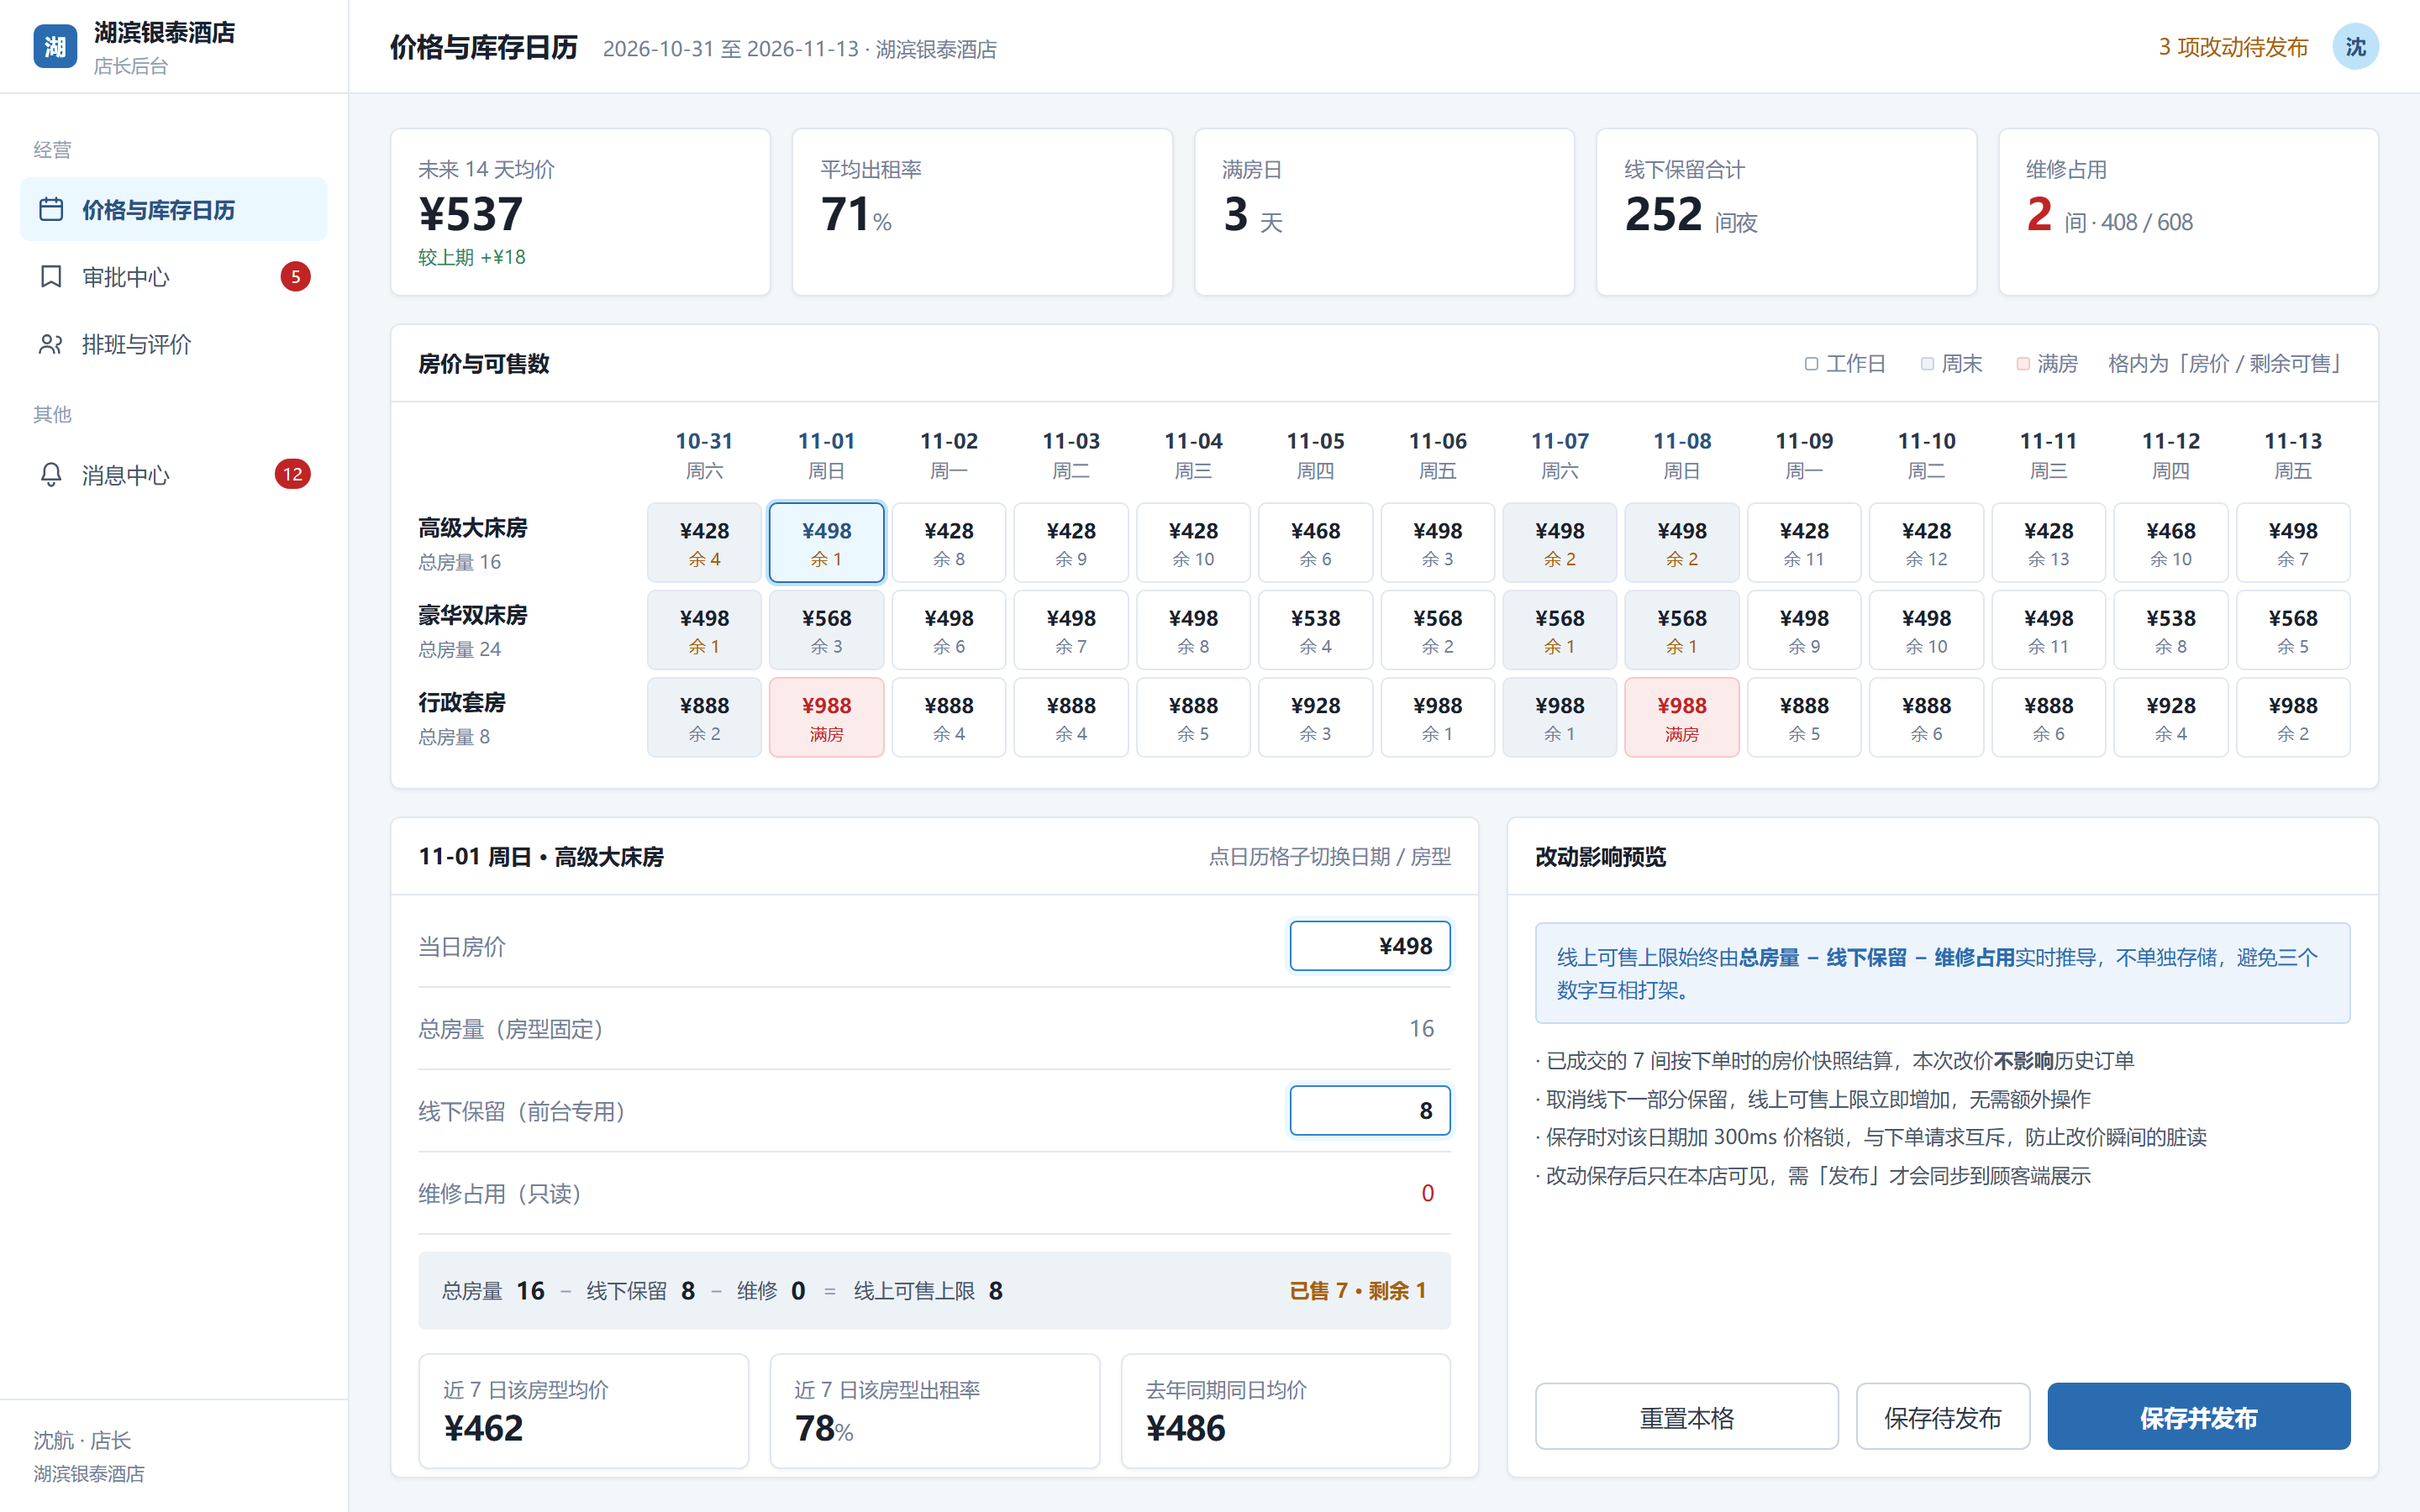
\includegraphics[width=\textwidth]{../UI界面/12_price_calendar.png}
  \caption{价格与库存日历}
\end{subfigure}\\[3pt]
\begin{subfigure}[b]{0.95\textwidth}
  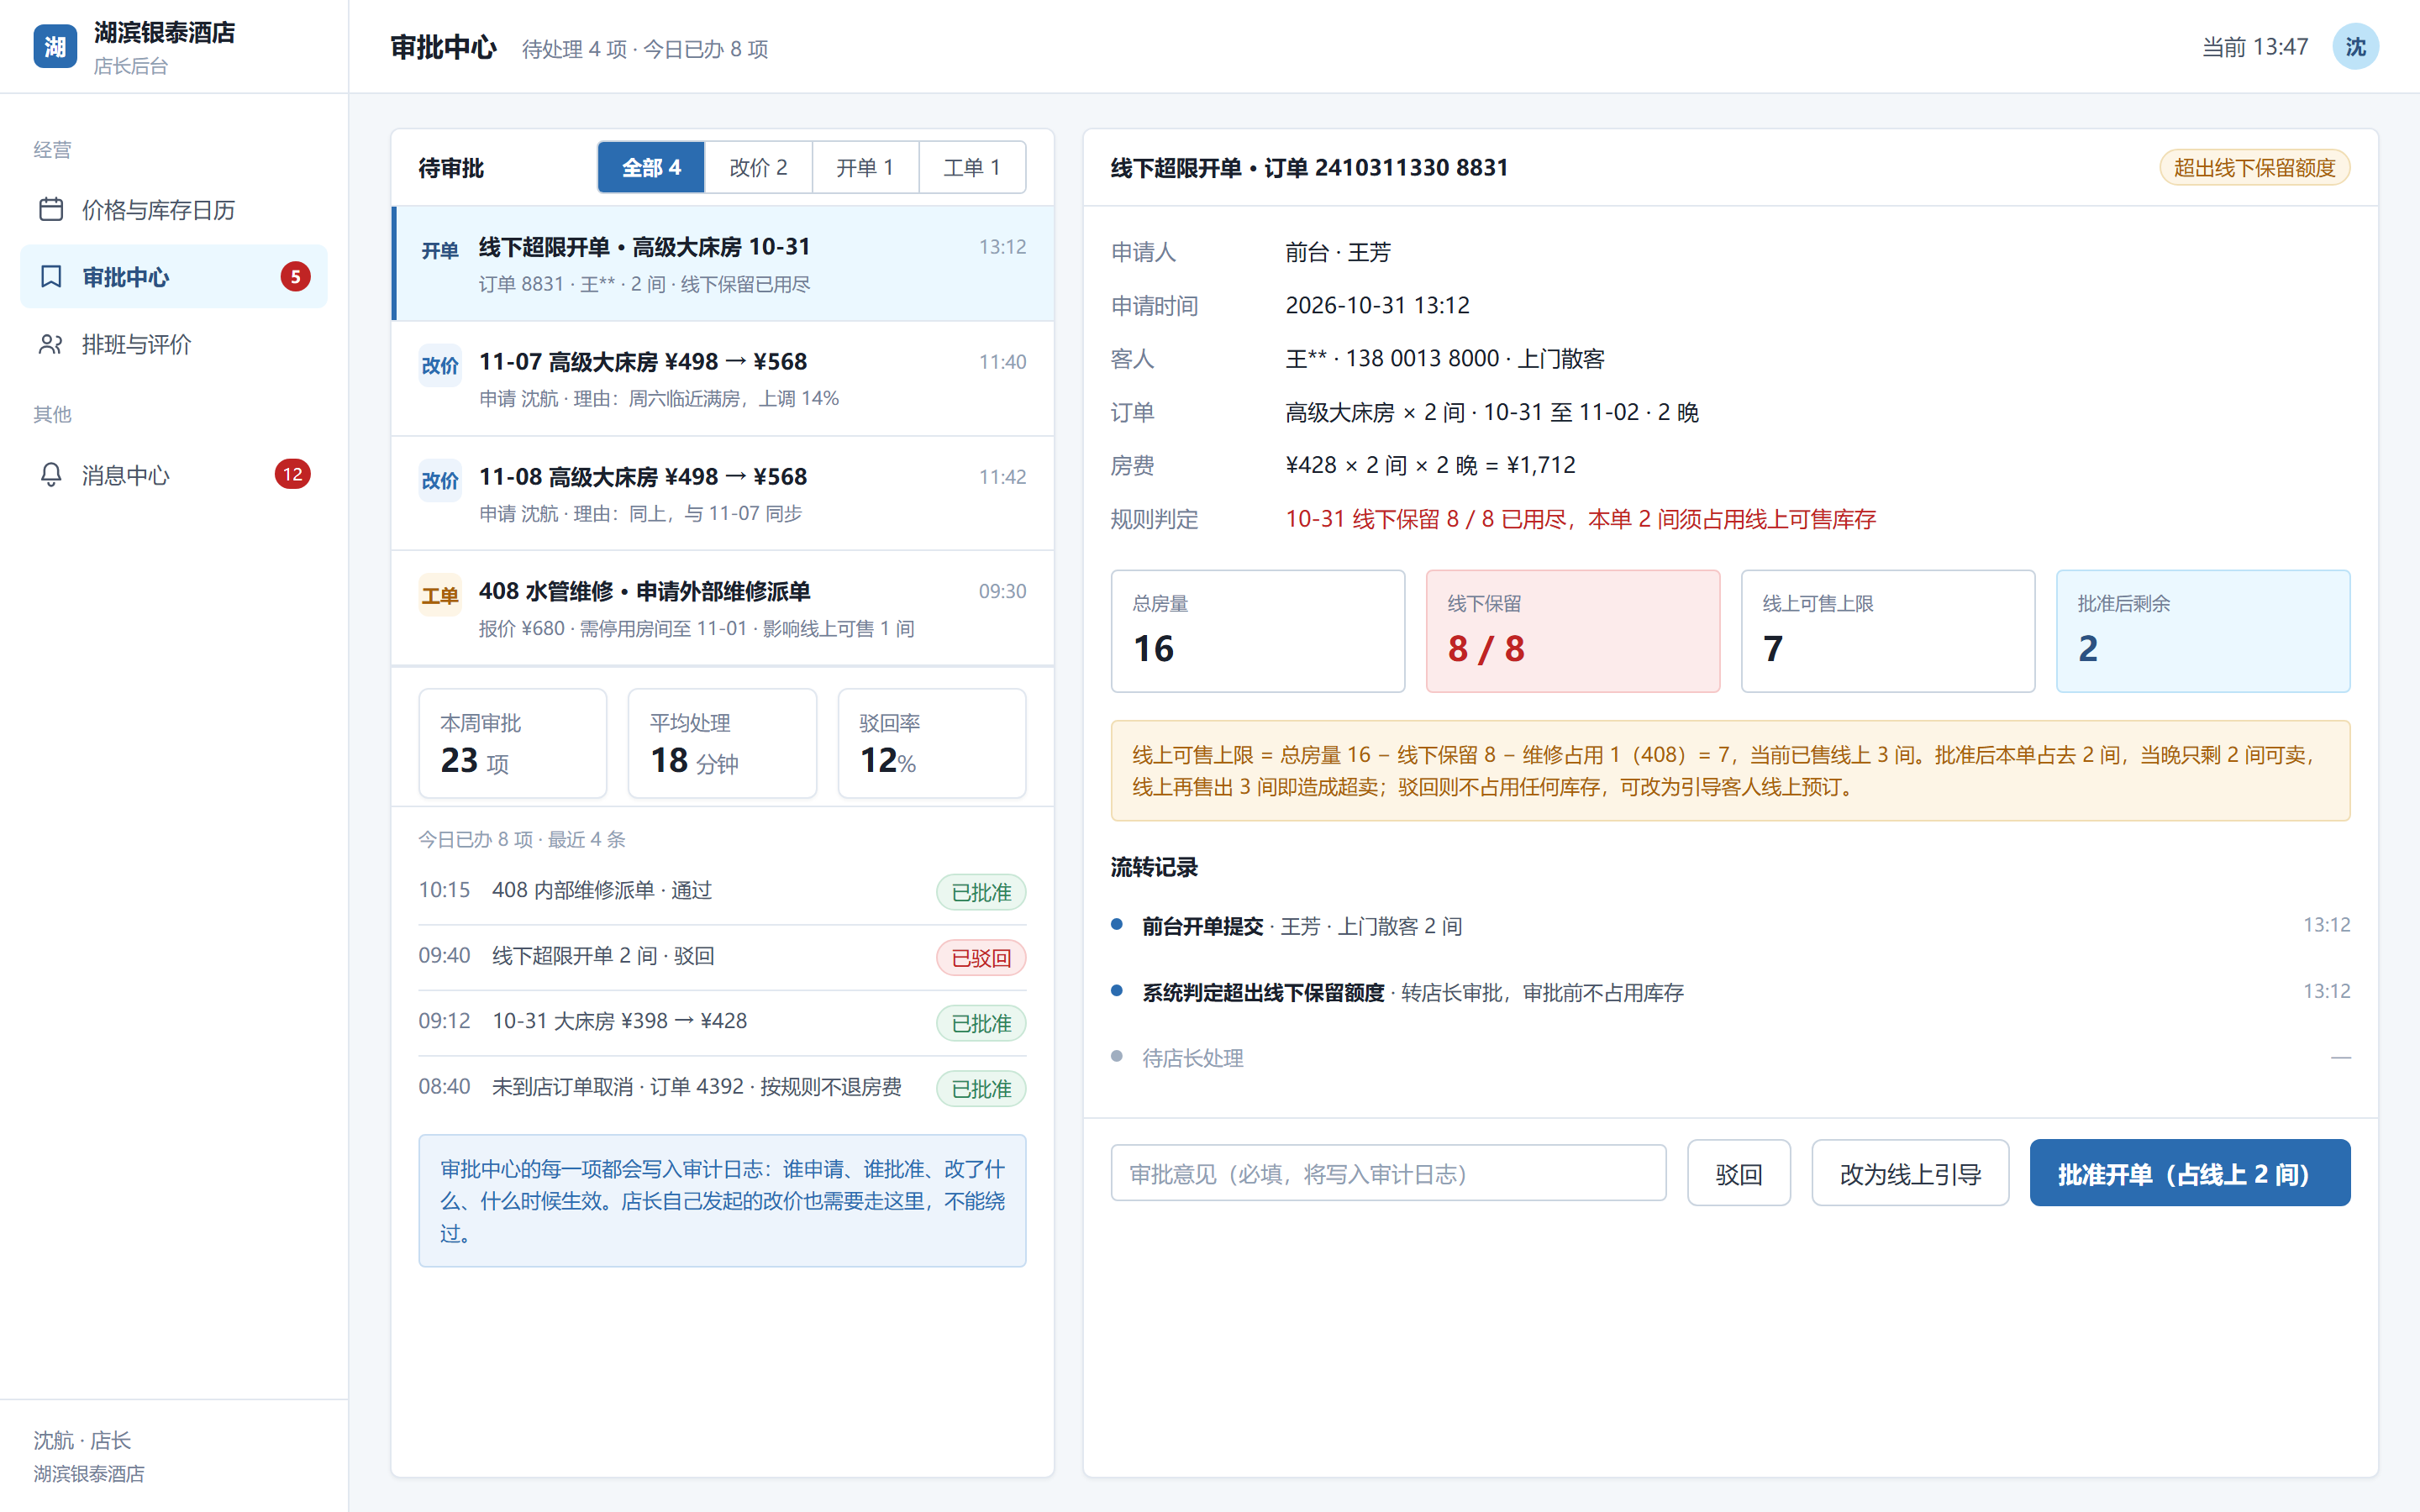
\includegraphics[width=\textwidth]{../UI界面/13_approval_center.png}
  \caption{审批中心}
\end{subfigure}
\caption{店长端：定价与审批（12--13）}
\label{fig:ui_m1}
\end{figure}

\textbf{12 价格与库存日历。} 按房型与日期展示未来 14 天日价、线上余量和线下保留额度；店长可调整价格与可售上限。维修占用与待发布修改单独汇总（REQ-006、REQ-013、REQ-033）。

\textbf{13 审批中心。} 按改价、超限开单和工单类型列出待办；选中申请后展示金额、库存影响及申请理由。审批意见必填，批准或驳回均记录审计日志（REQ-014）。

\begin{figure}[htbp]
\centering
\begin{subfigure}[b]{0.95\textwidth}
  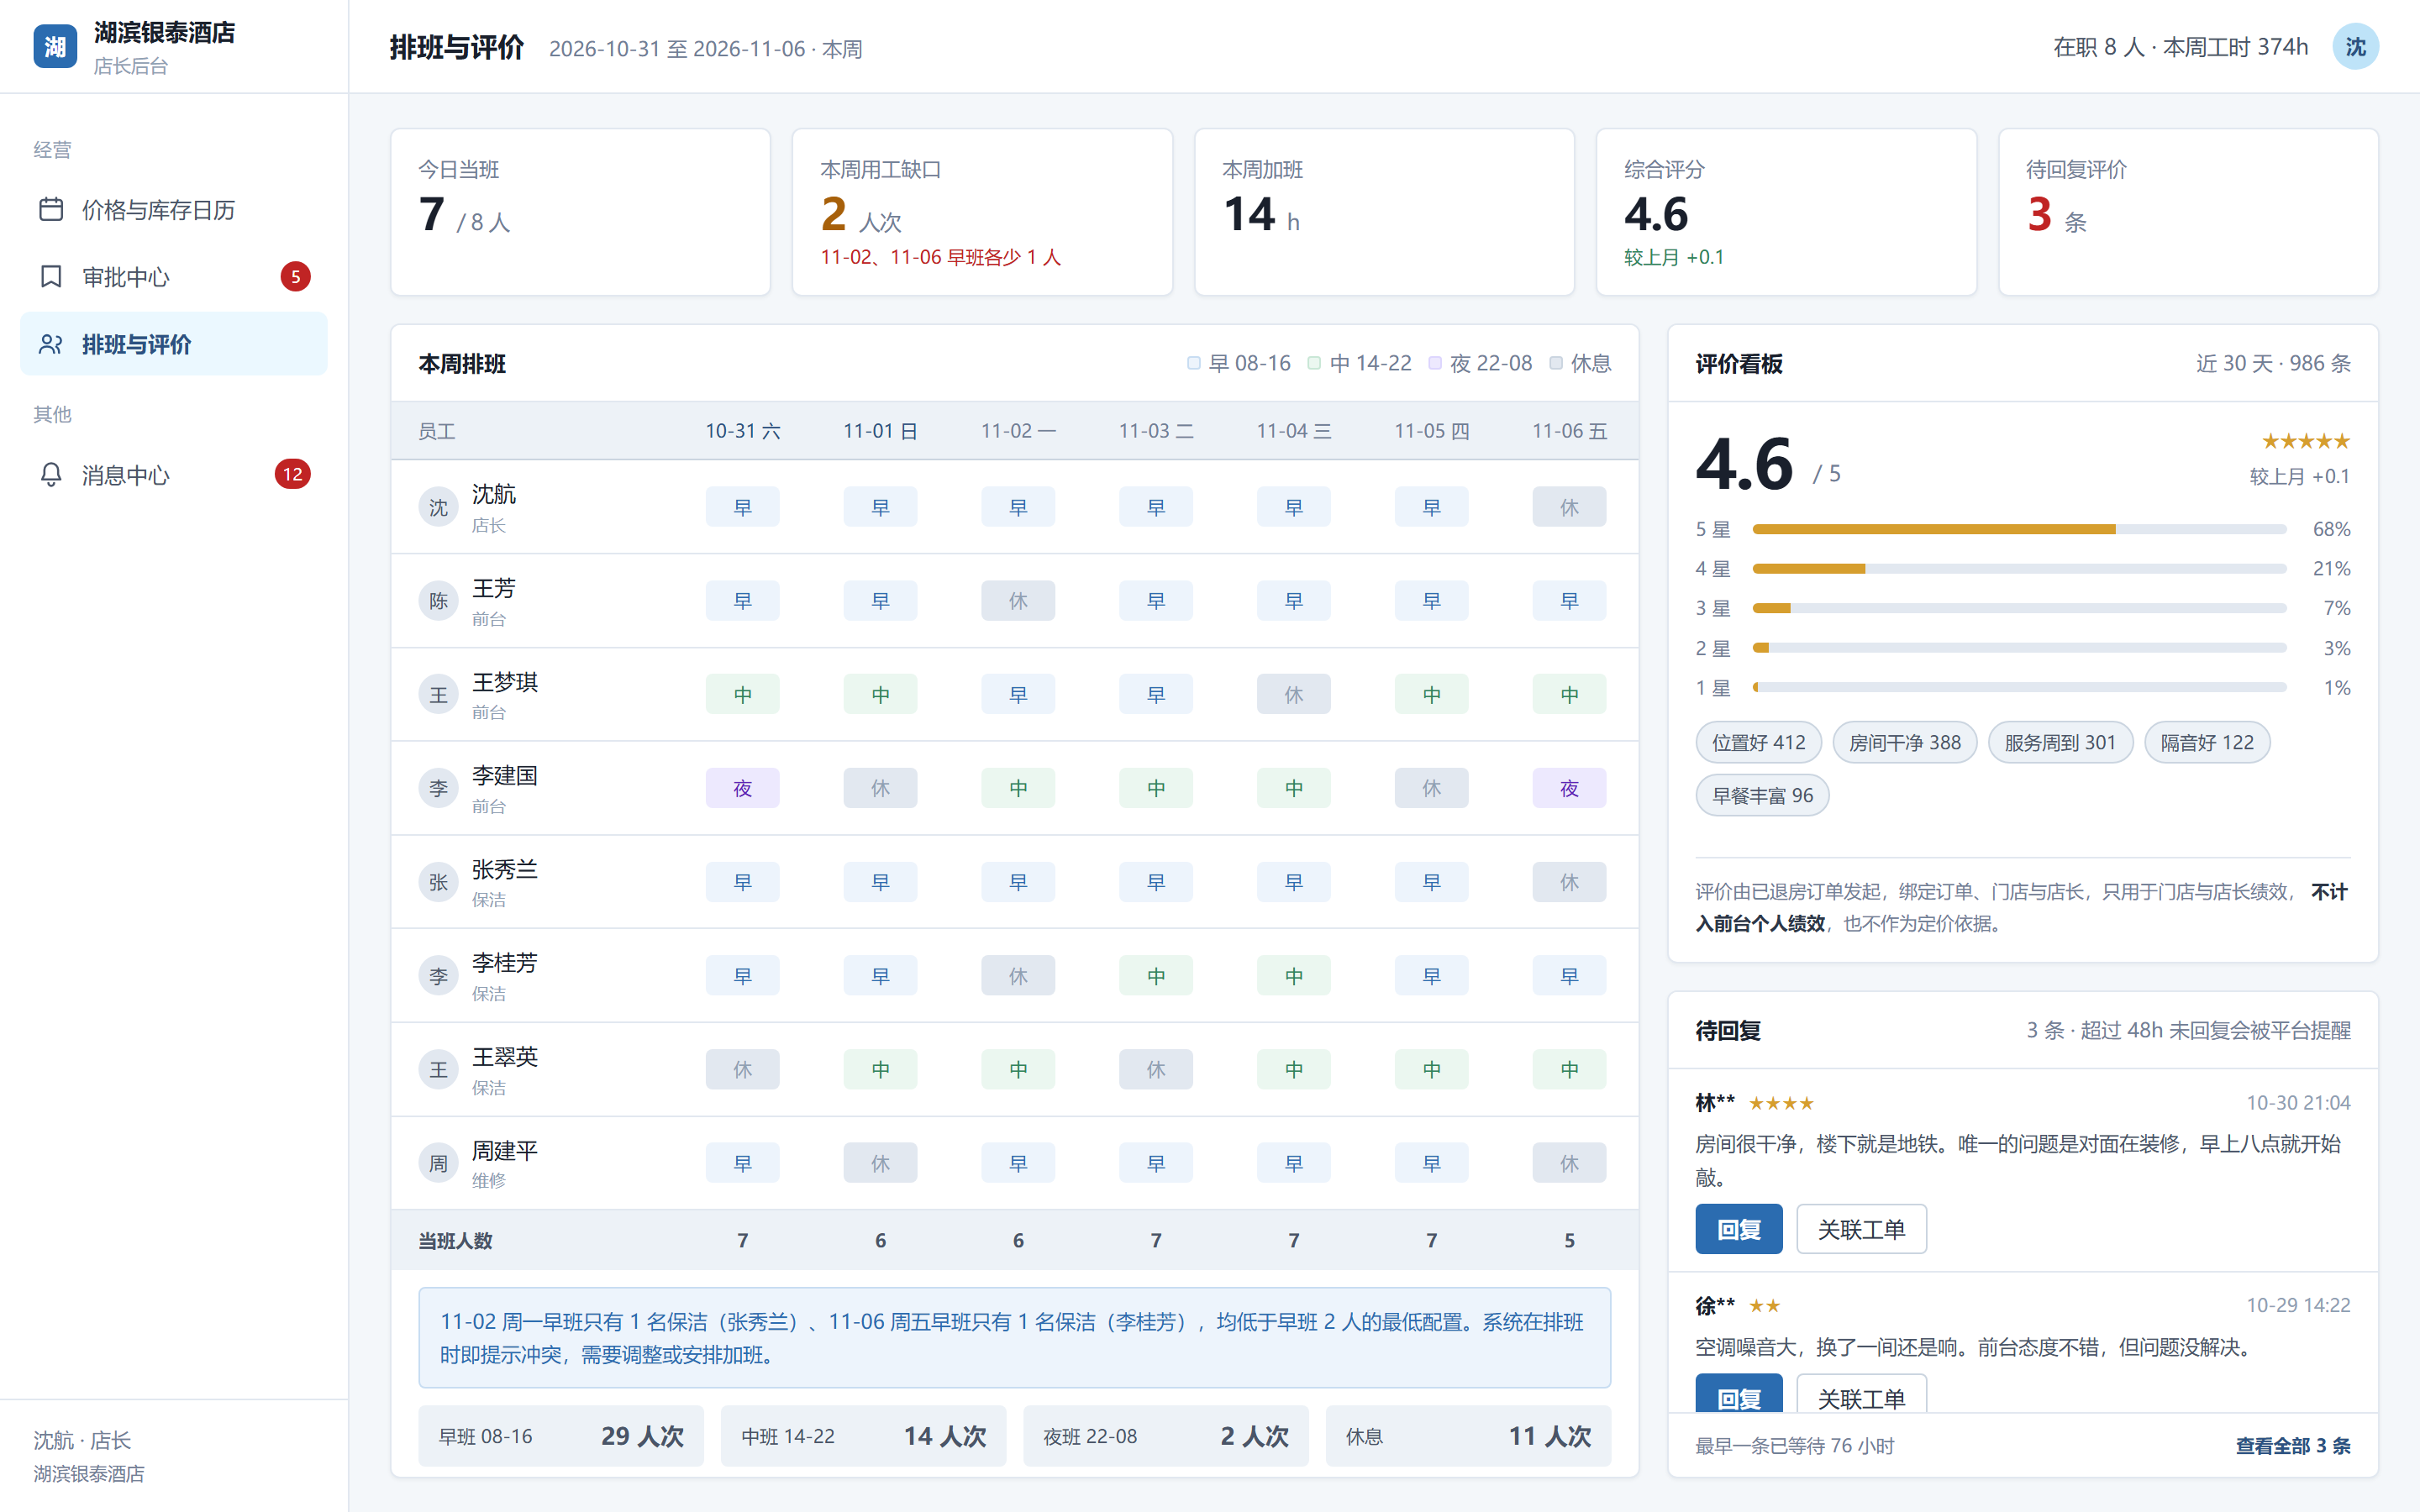
\includegraphics[width=\textwidth]{../UI界面/14_roster_review.png}
  \caption{排班与评价}
\end{subfigure}
\caption{店长端：排班与评价（14）}
\label{fig:ui_m2}
\end{figure}

\textbf{14 排班与评价。} 以周视图安排本店员工班次，标出缺岗日期；同屏展示综合评分和待回复评价。店长仅查看本店人员信息（REQ-026）。

\begin{figure}[htbp]
\centering
\begin{subfigure}[b]{0.95\textwidth}
  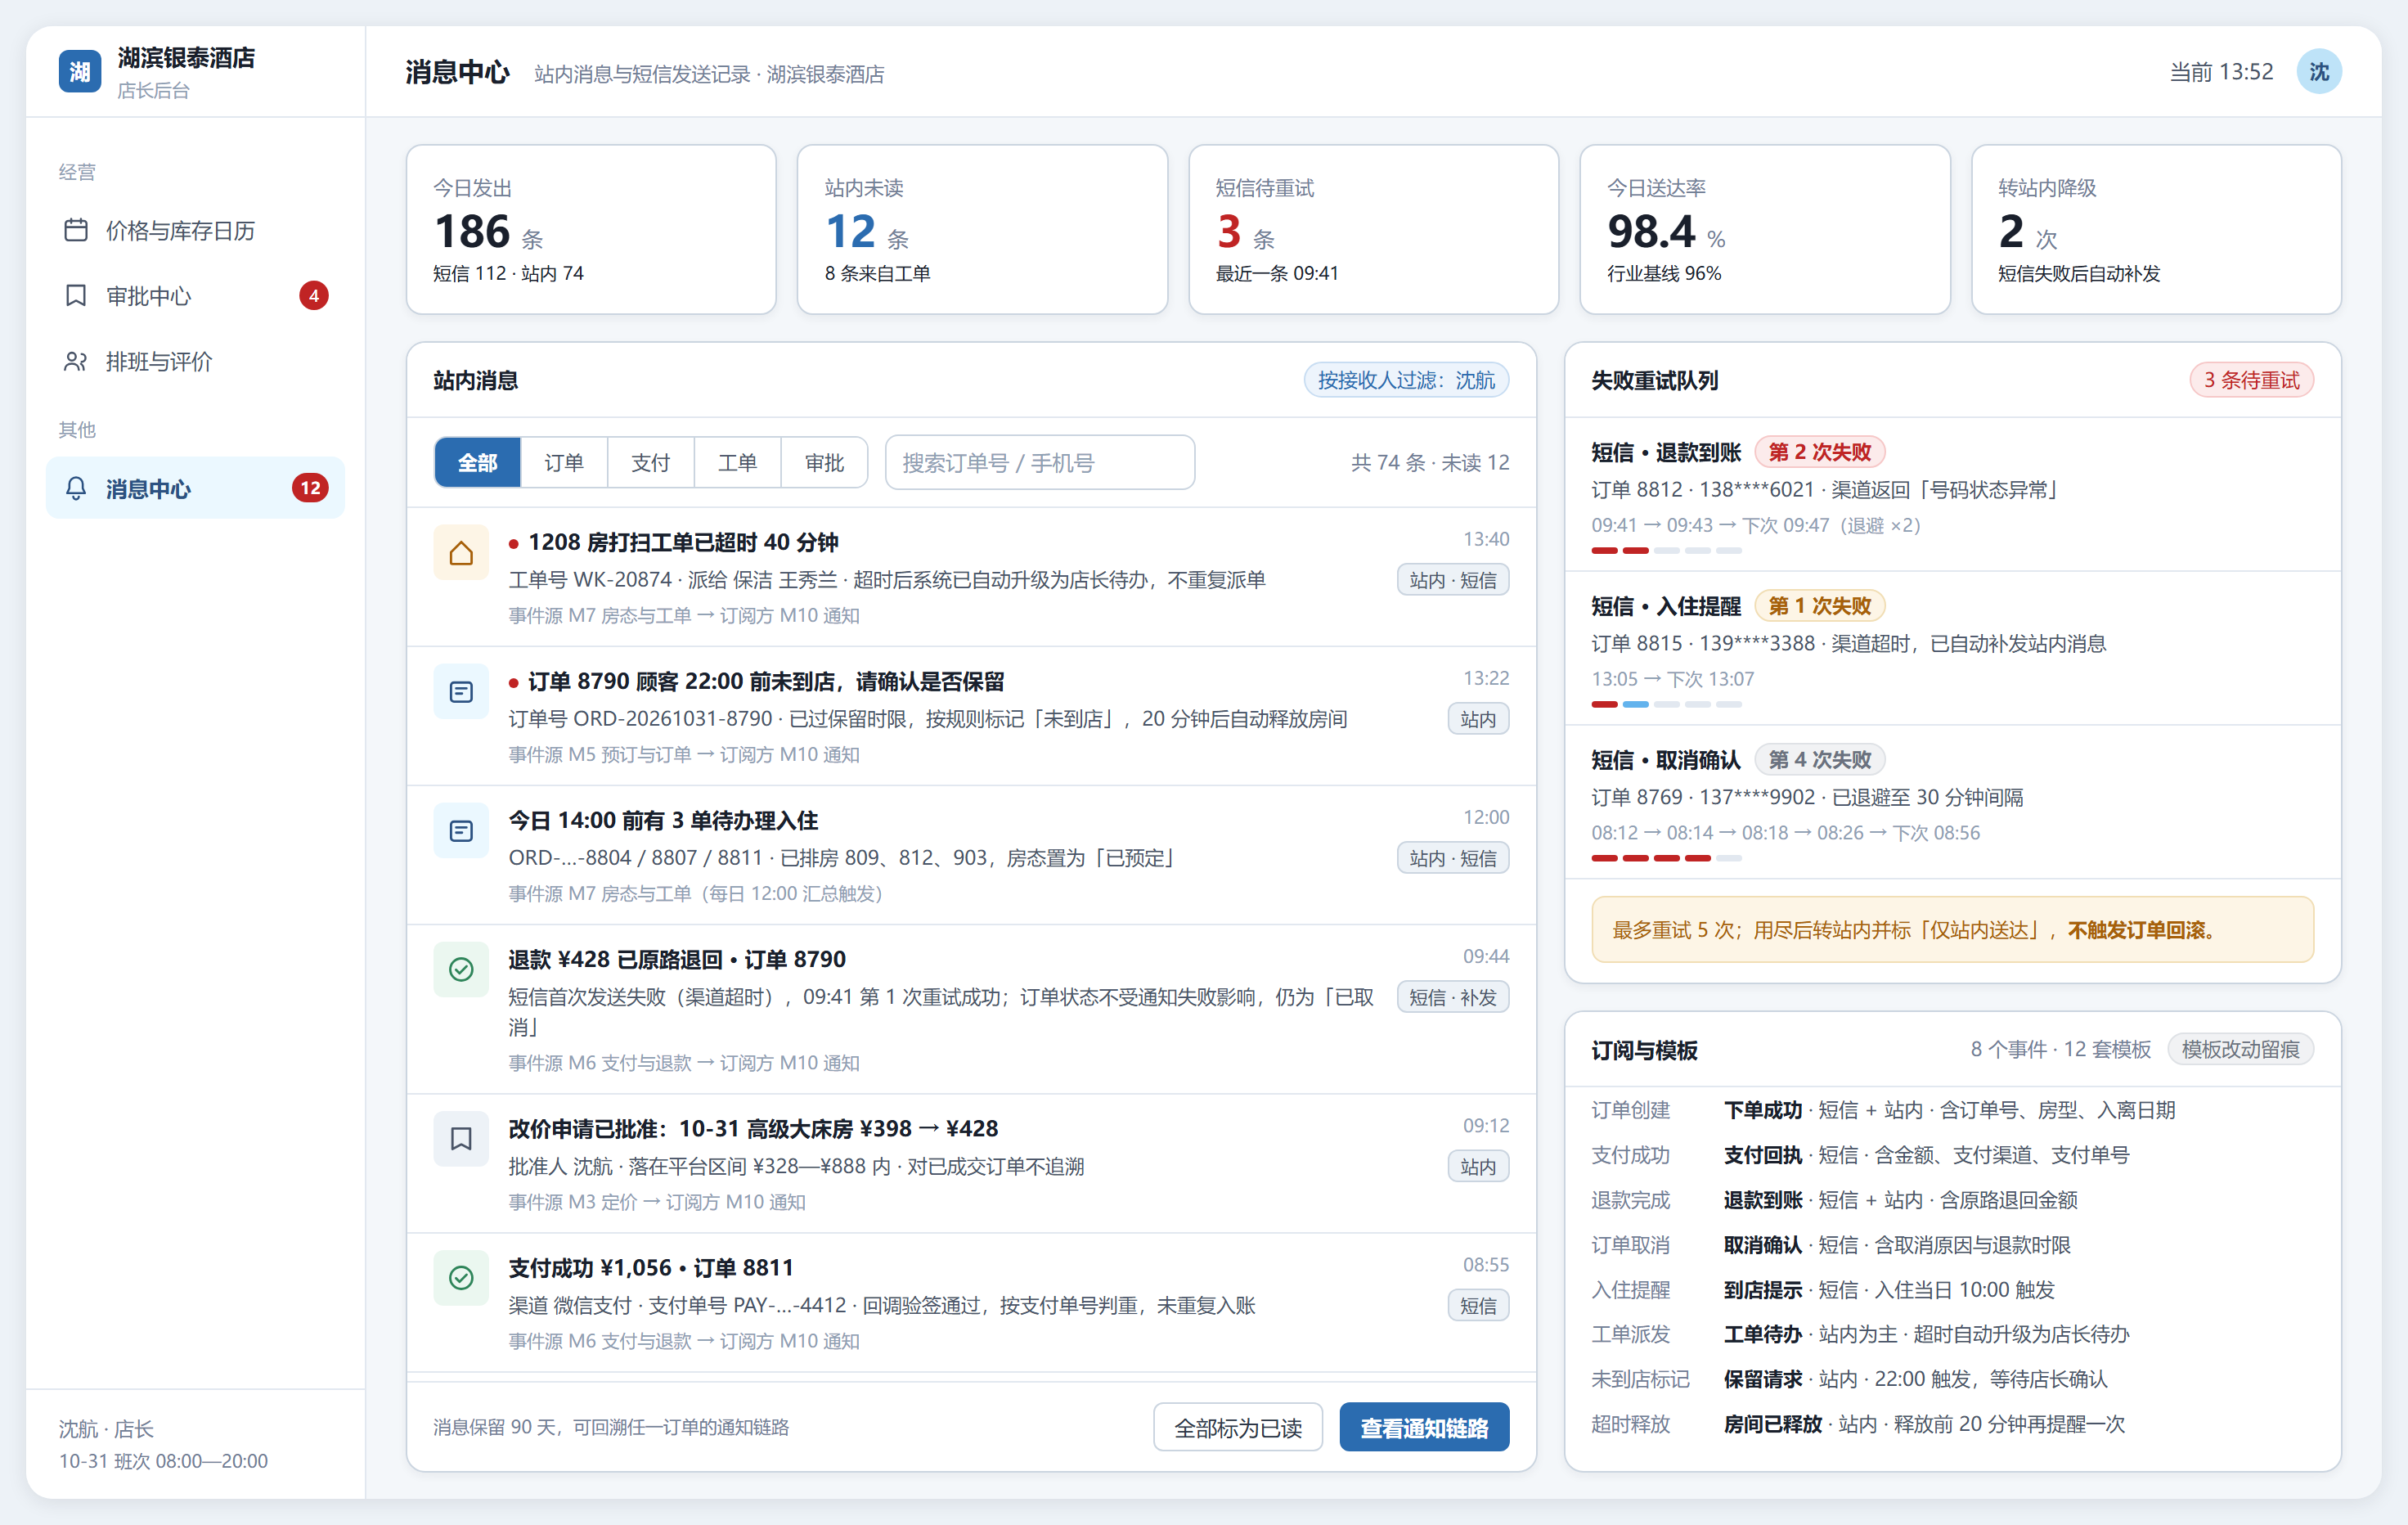
\includegraphics[width=\textwidth]{../UI界面/17_message_center.png}
  \caption{消息中心：站内消息、失败重试与订阅规则}
\end{subfigure}
\caption{店长端：消息中心（17）}
\label{fig:ui_m3}
\end{figure}

\textbf{17 消息中心。} 查询站内消息、短信发送状态与失败重试队列。通知最多重试五次，失败后转站内消息，不回滚订单；模板修改留痕（REQ-029）。

\subsection{平台端（4 屏，桌面后台）}

平台端提供跨店汇总、价格区间下发、人员调动和审计查询；不提供办理入住或修改房态入口（REQ-007）。

\begin{figure}[htbp]
\centering
\begin{subfigure}[b]{0.95\textwidth}
  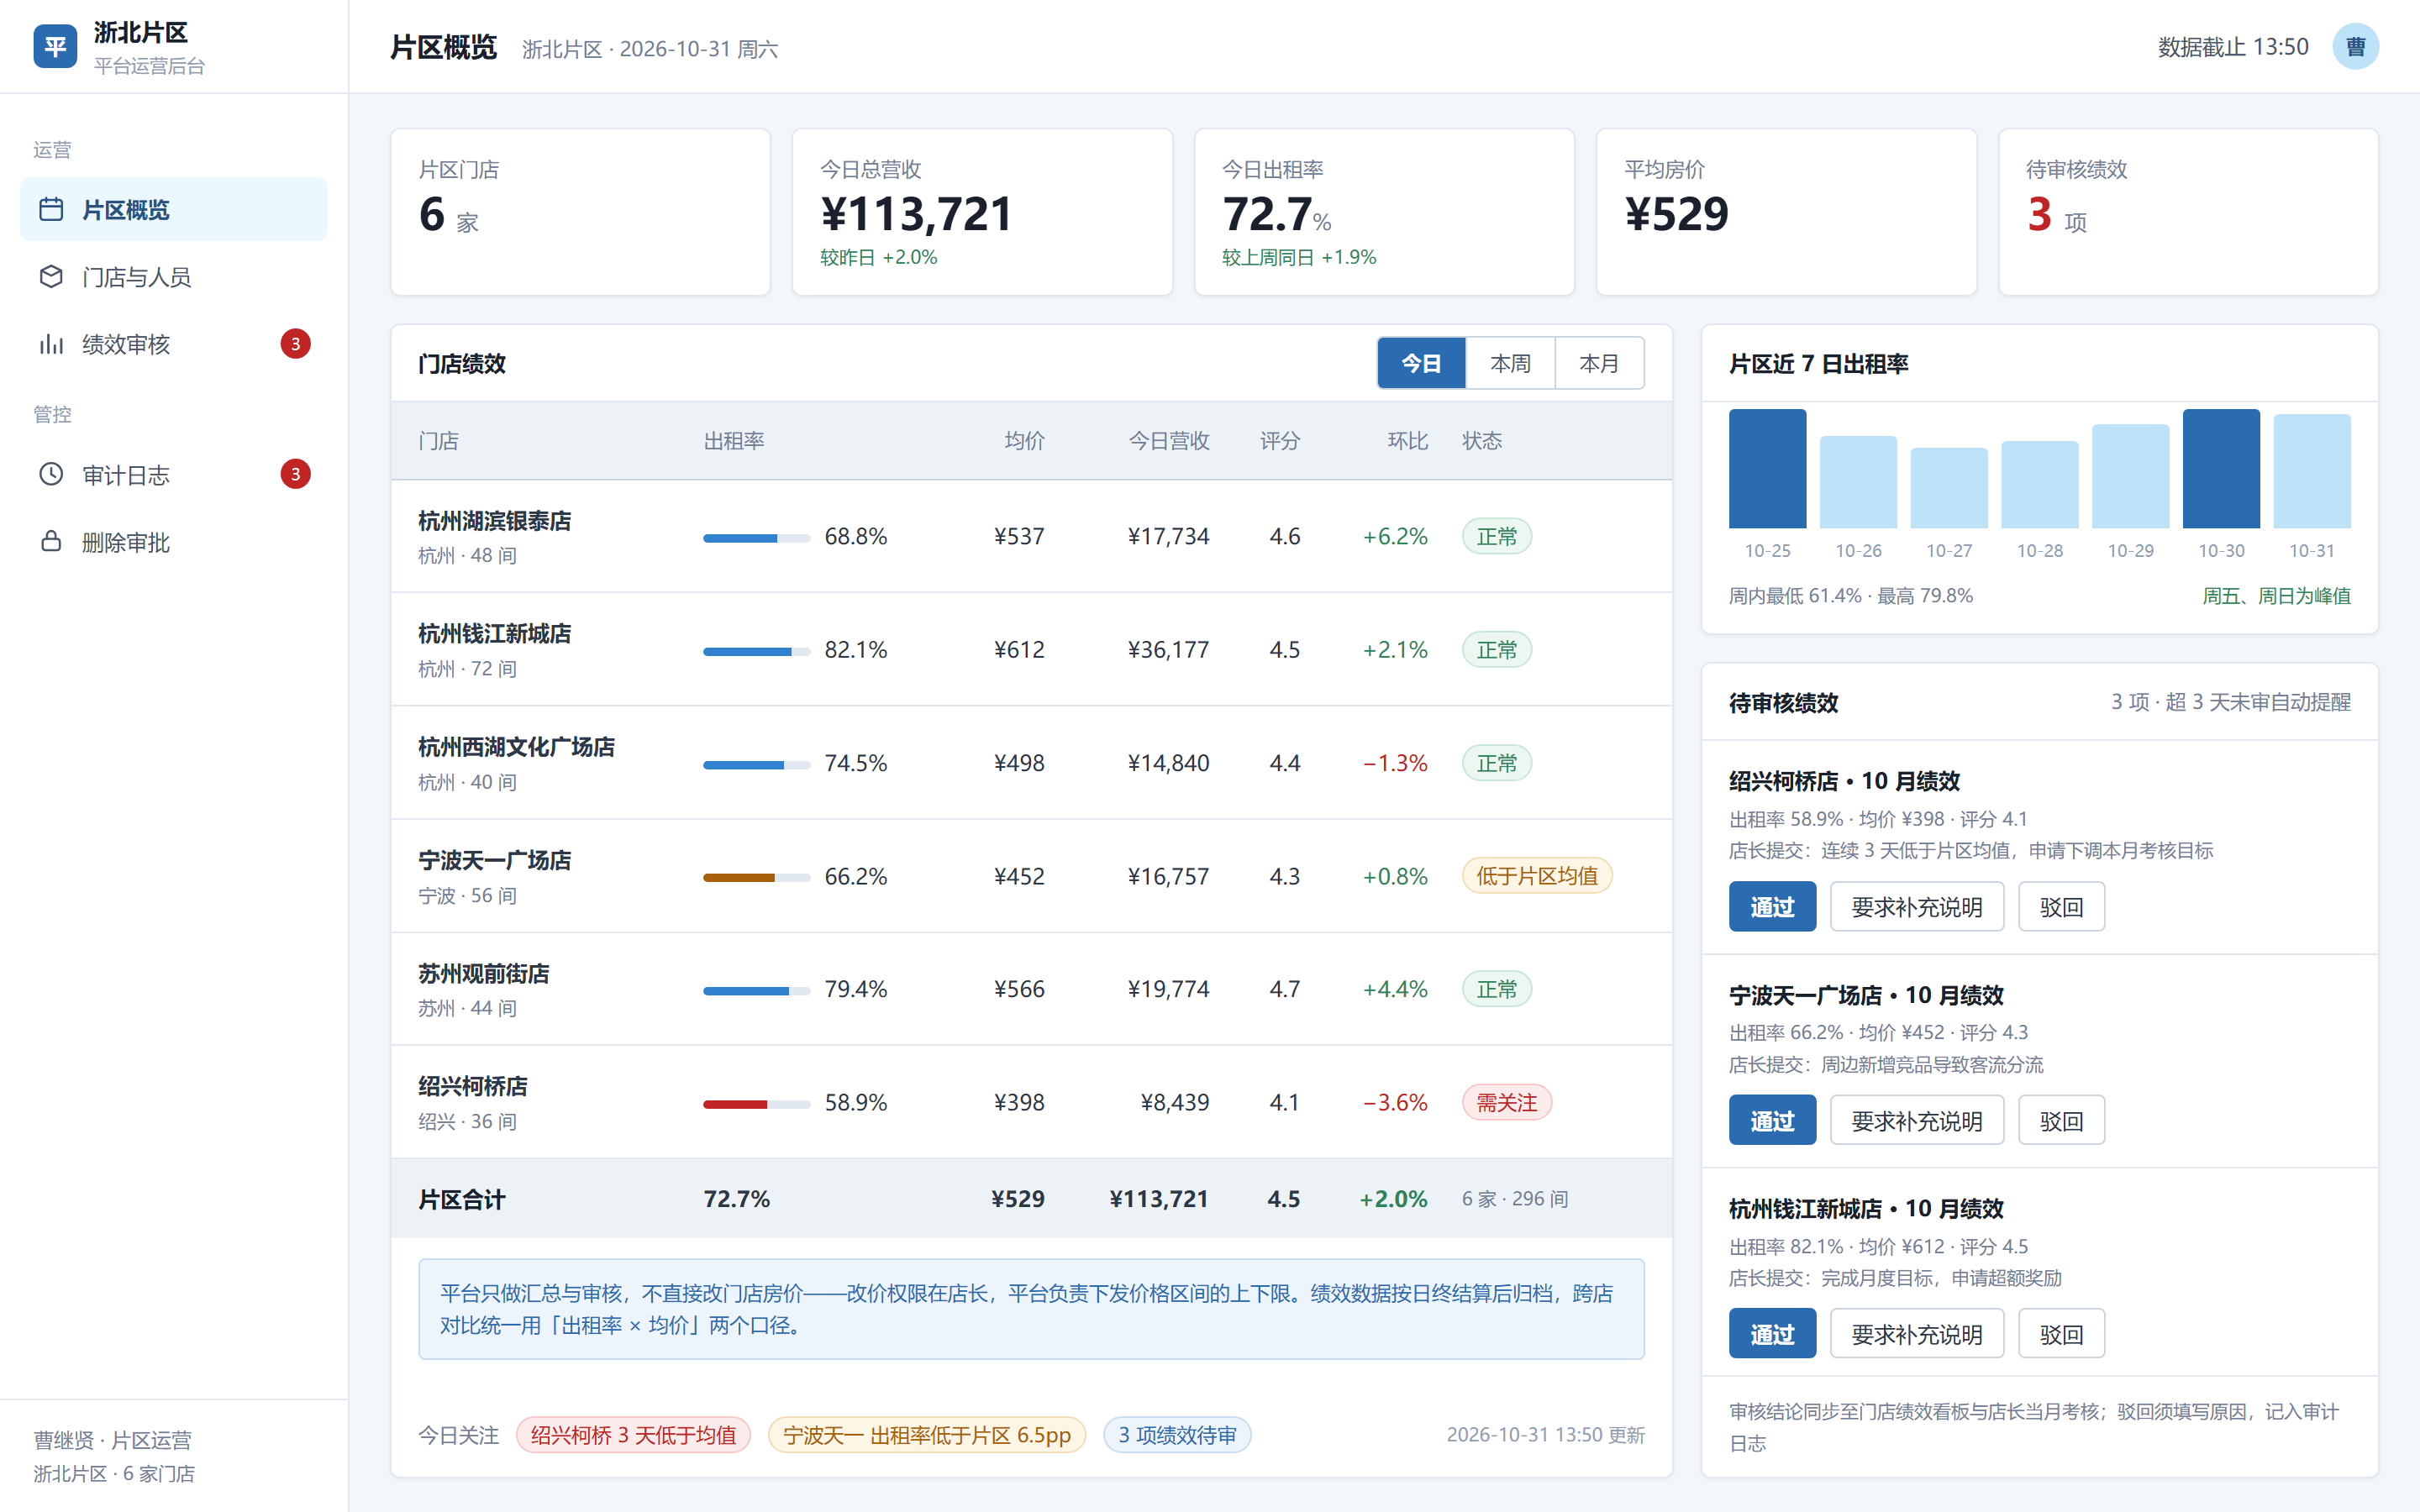
\includegraphics[width=\textwidth]{../UI界面/15_region_overview.png}
  \caption{片区概览与门店绩效}
\end{subfigure}\\[3pt]
\begin{subfigure}[b]{0.95\textwidth}
  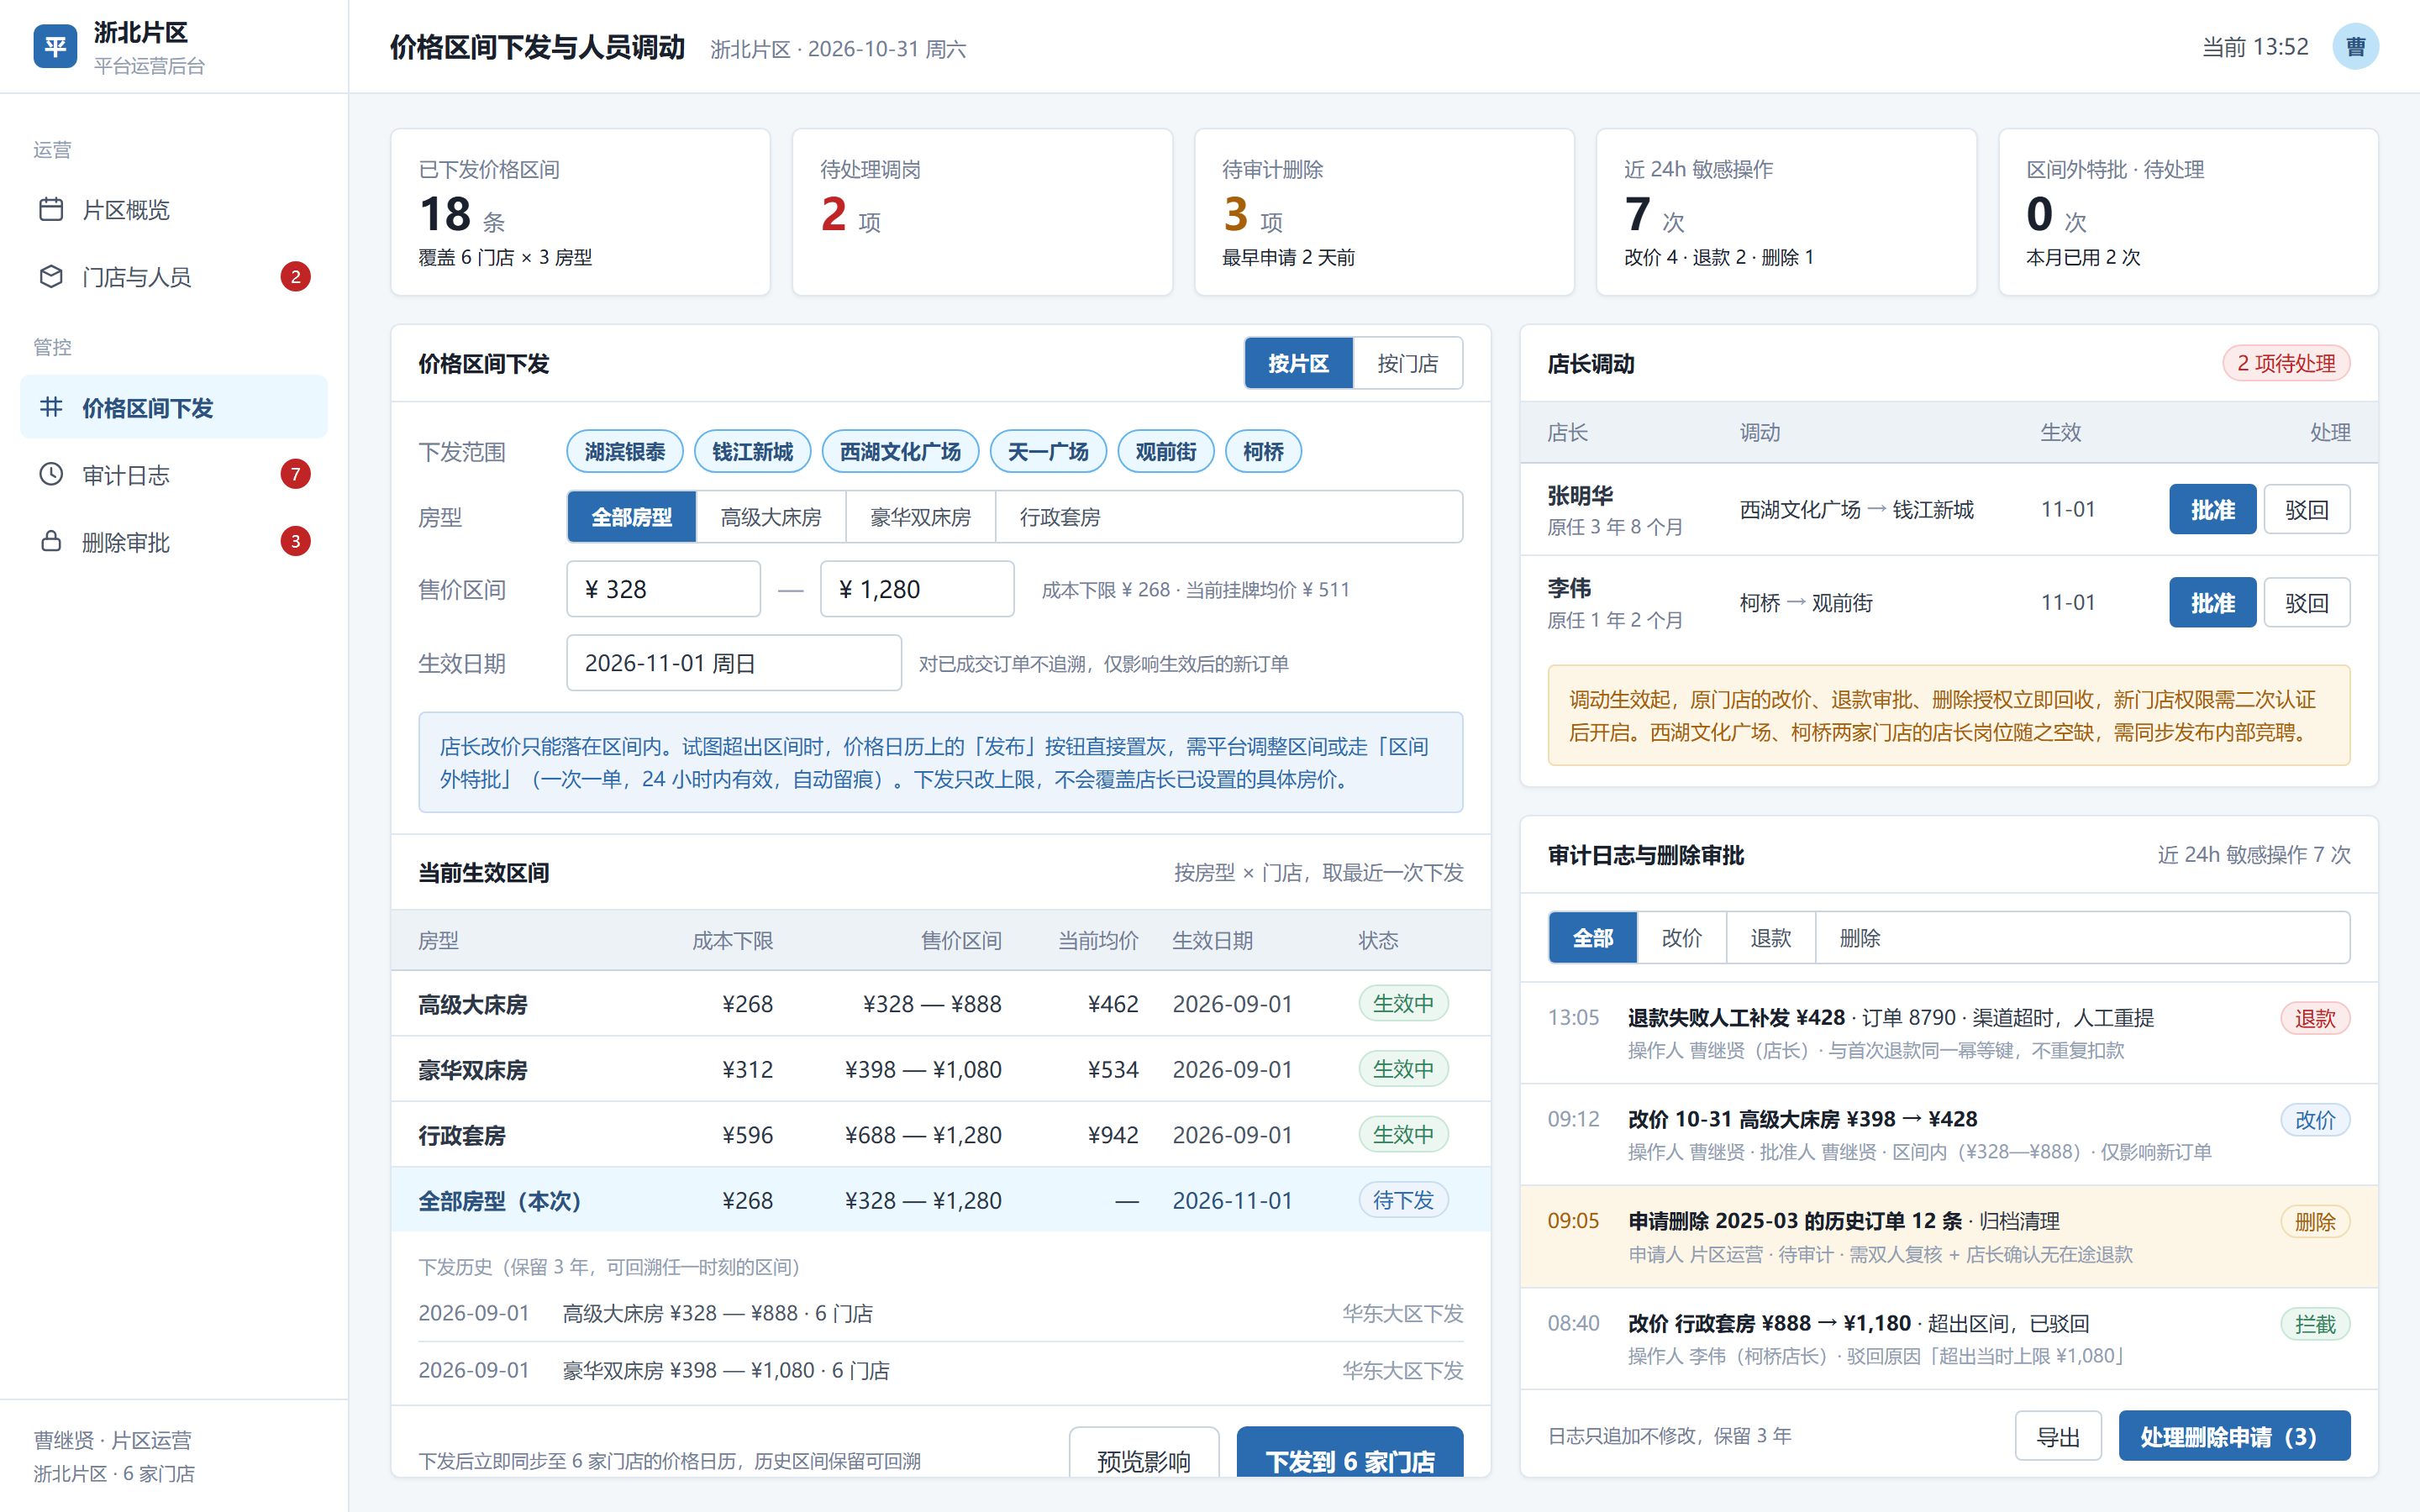
\includegraphics[width=\textwidth]{../UI界面/16_price_range_staffing.png}
  \caption{价格区间下发、人员调动与审计}
\end{subfigure}
\caption{平台端：片区概览与管控（15--16）}
\label{fig:ui_p}
\end{figure}

\textbf{15 片区概览与门店绩效。} 汇总六家门店的营收、出租率、均价和待审绩效；门店表展示各店评分及环比，右侧列出低于片区均值的门店。示例片区营收 ¥113,721、加权出租率 72.7\%。平台端只审核绩效，不直接修改门店房价（REQ-007）。

\textbf{16 价格区间下发、人员调动与审计。} 平台选择门店、房型、生效日期和价格区间，下发后只约束新订单，不改历史成交价（REQ-023）。同屏处理店长调动并查看敏感操作摘要；调动生效时回收原门店权限（REQ-007、REQ-014）。

\begin{figure}[htbp]
\centering
\begin{subfigure}[b]{0.95\textwidth}
  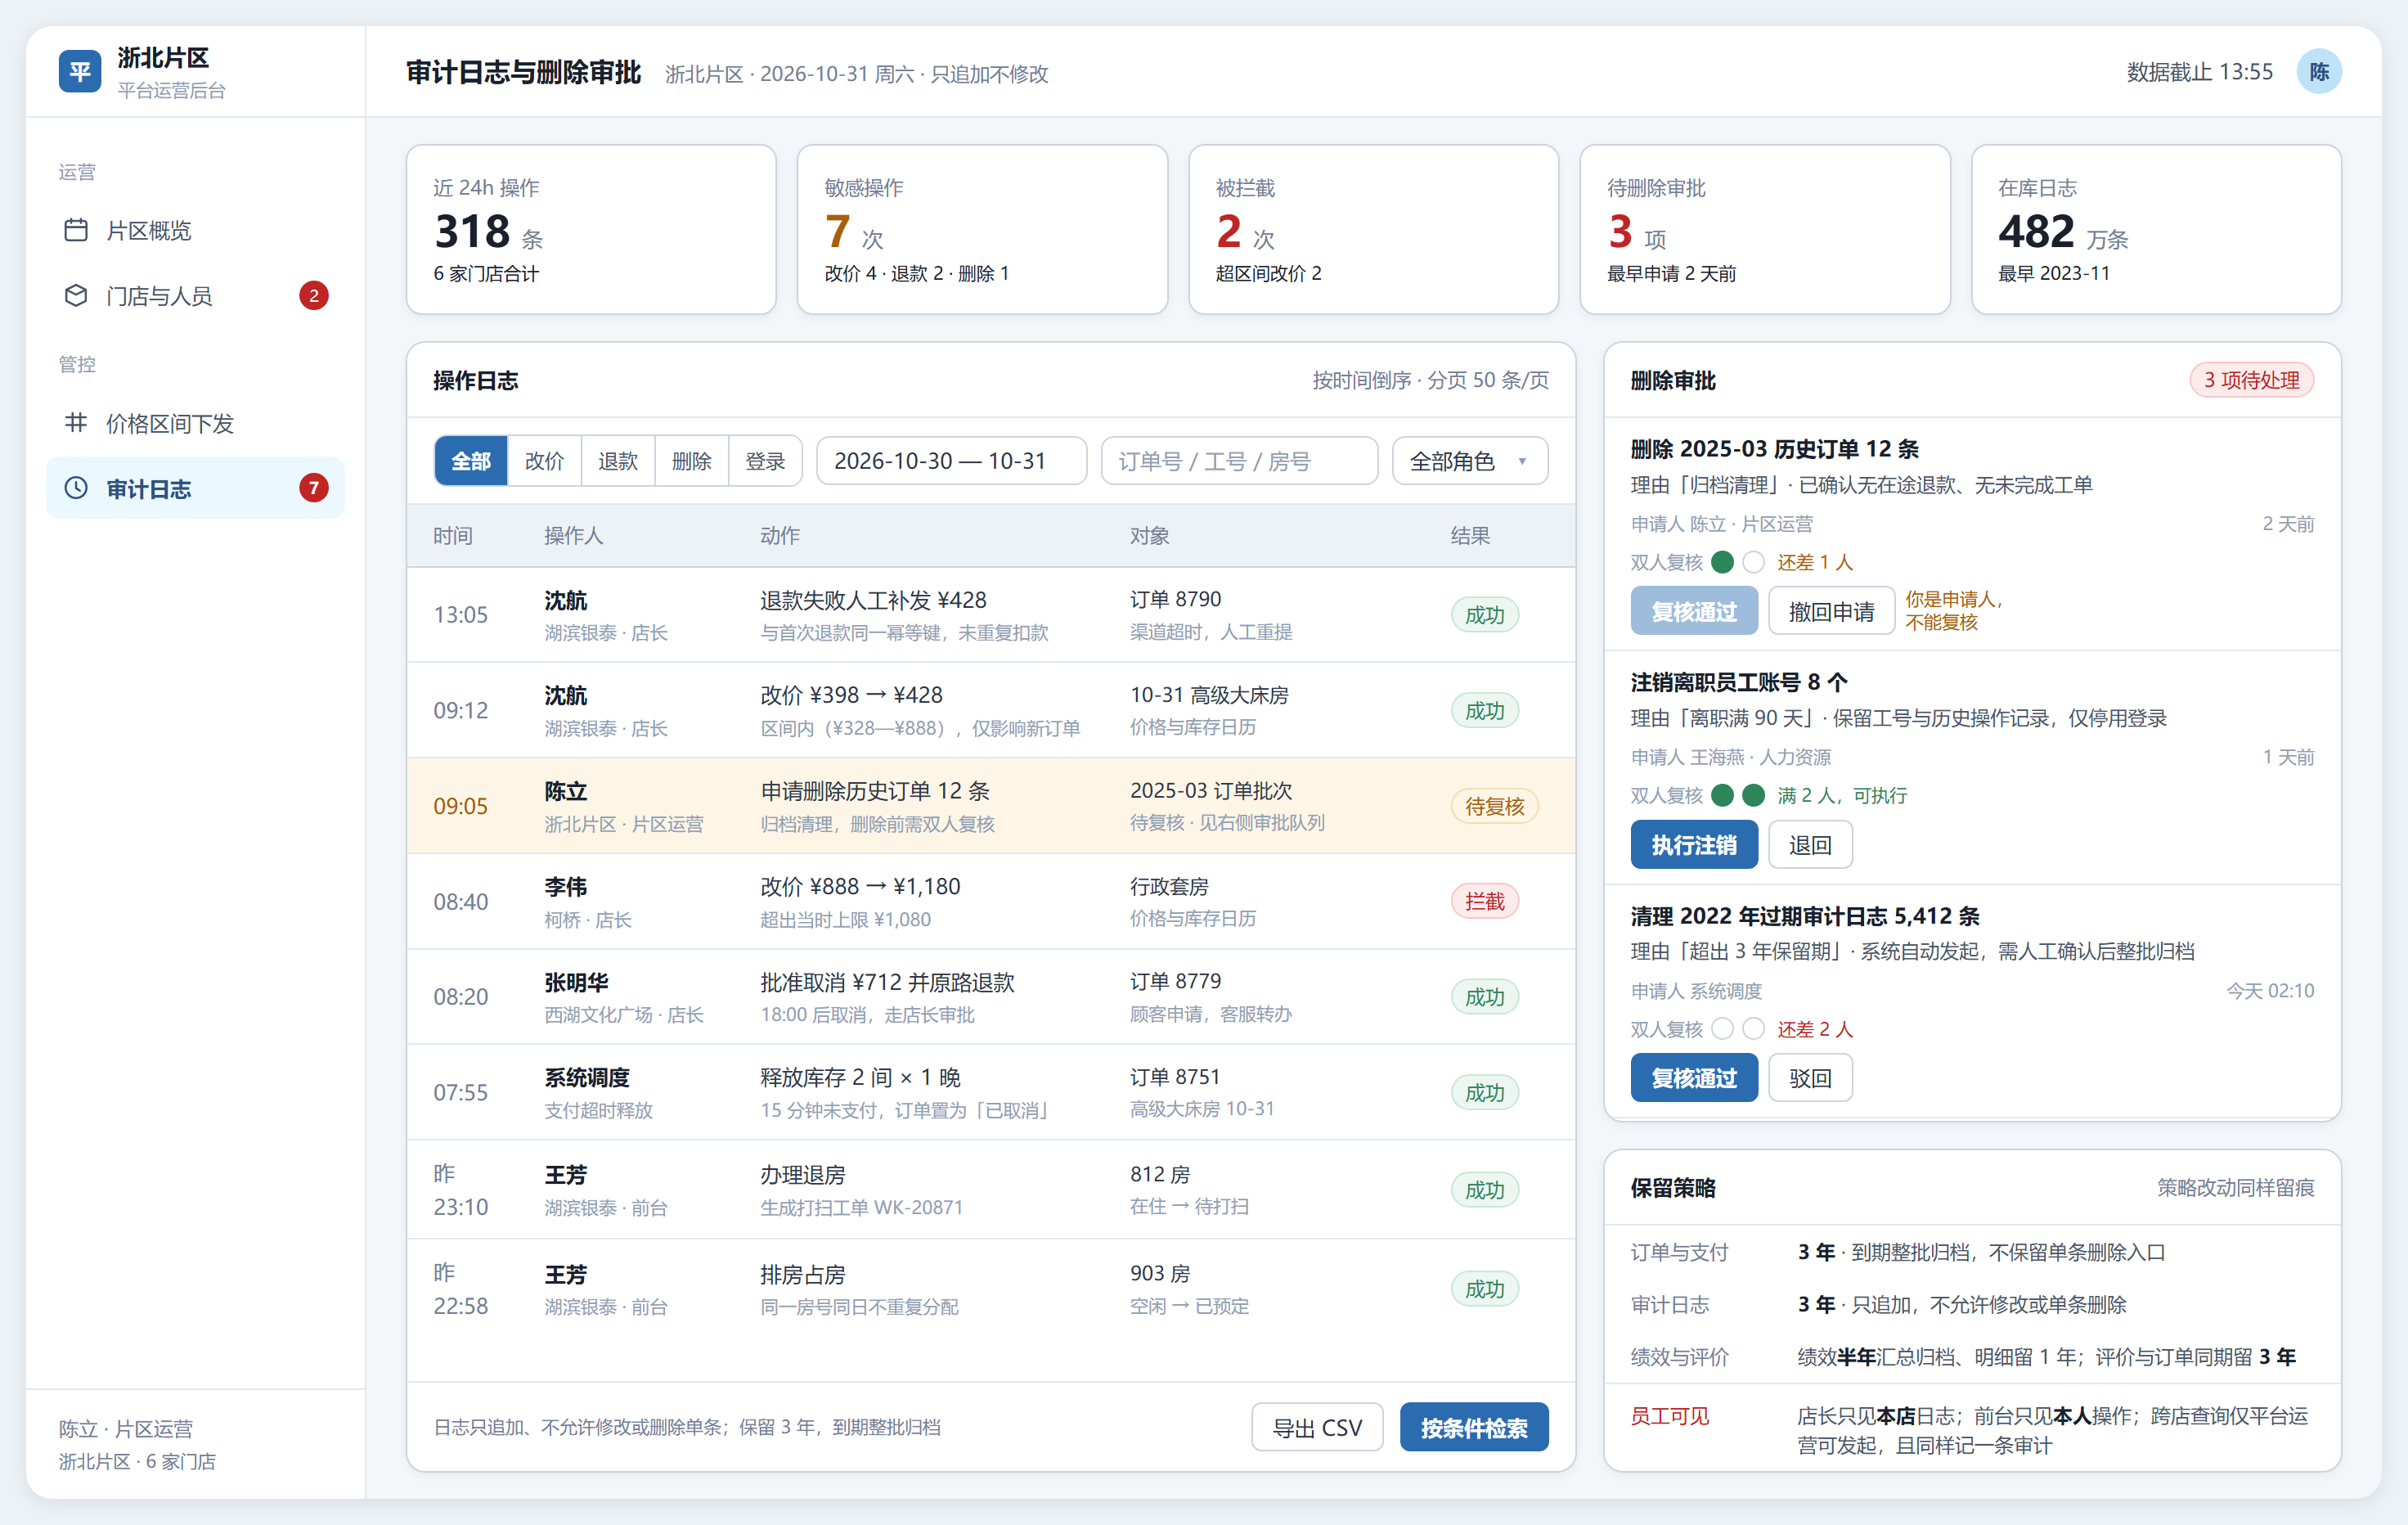
\includegraphics[width=\textwidth]{../UI界面/18_audit_log.png}
  \caption{审计日志与删除审批}
\end{subfigure}\\[3pt]
\begin{subfigure}[b]{0.95\textwidth}
  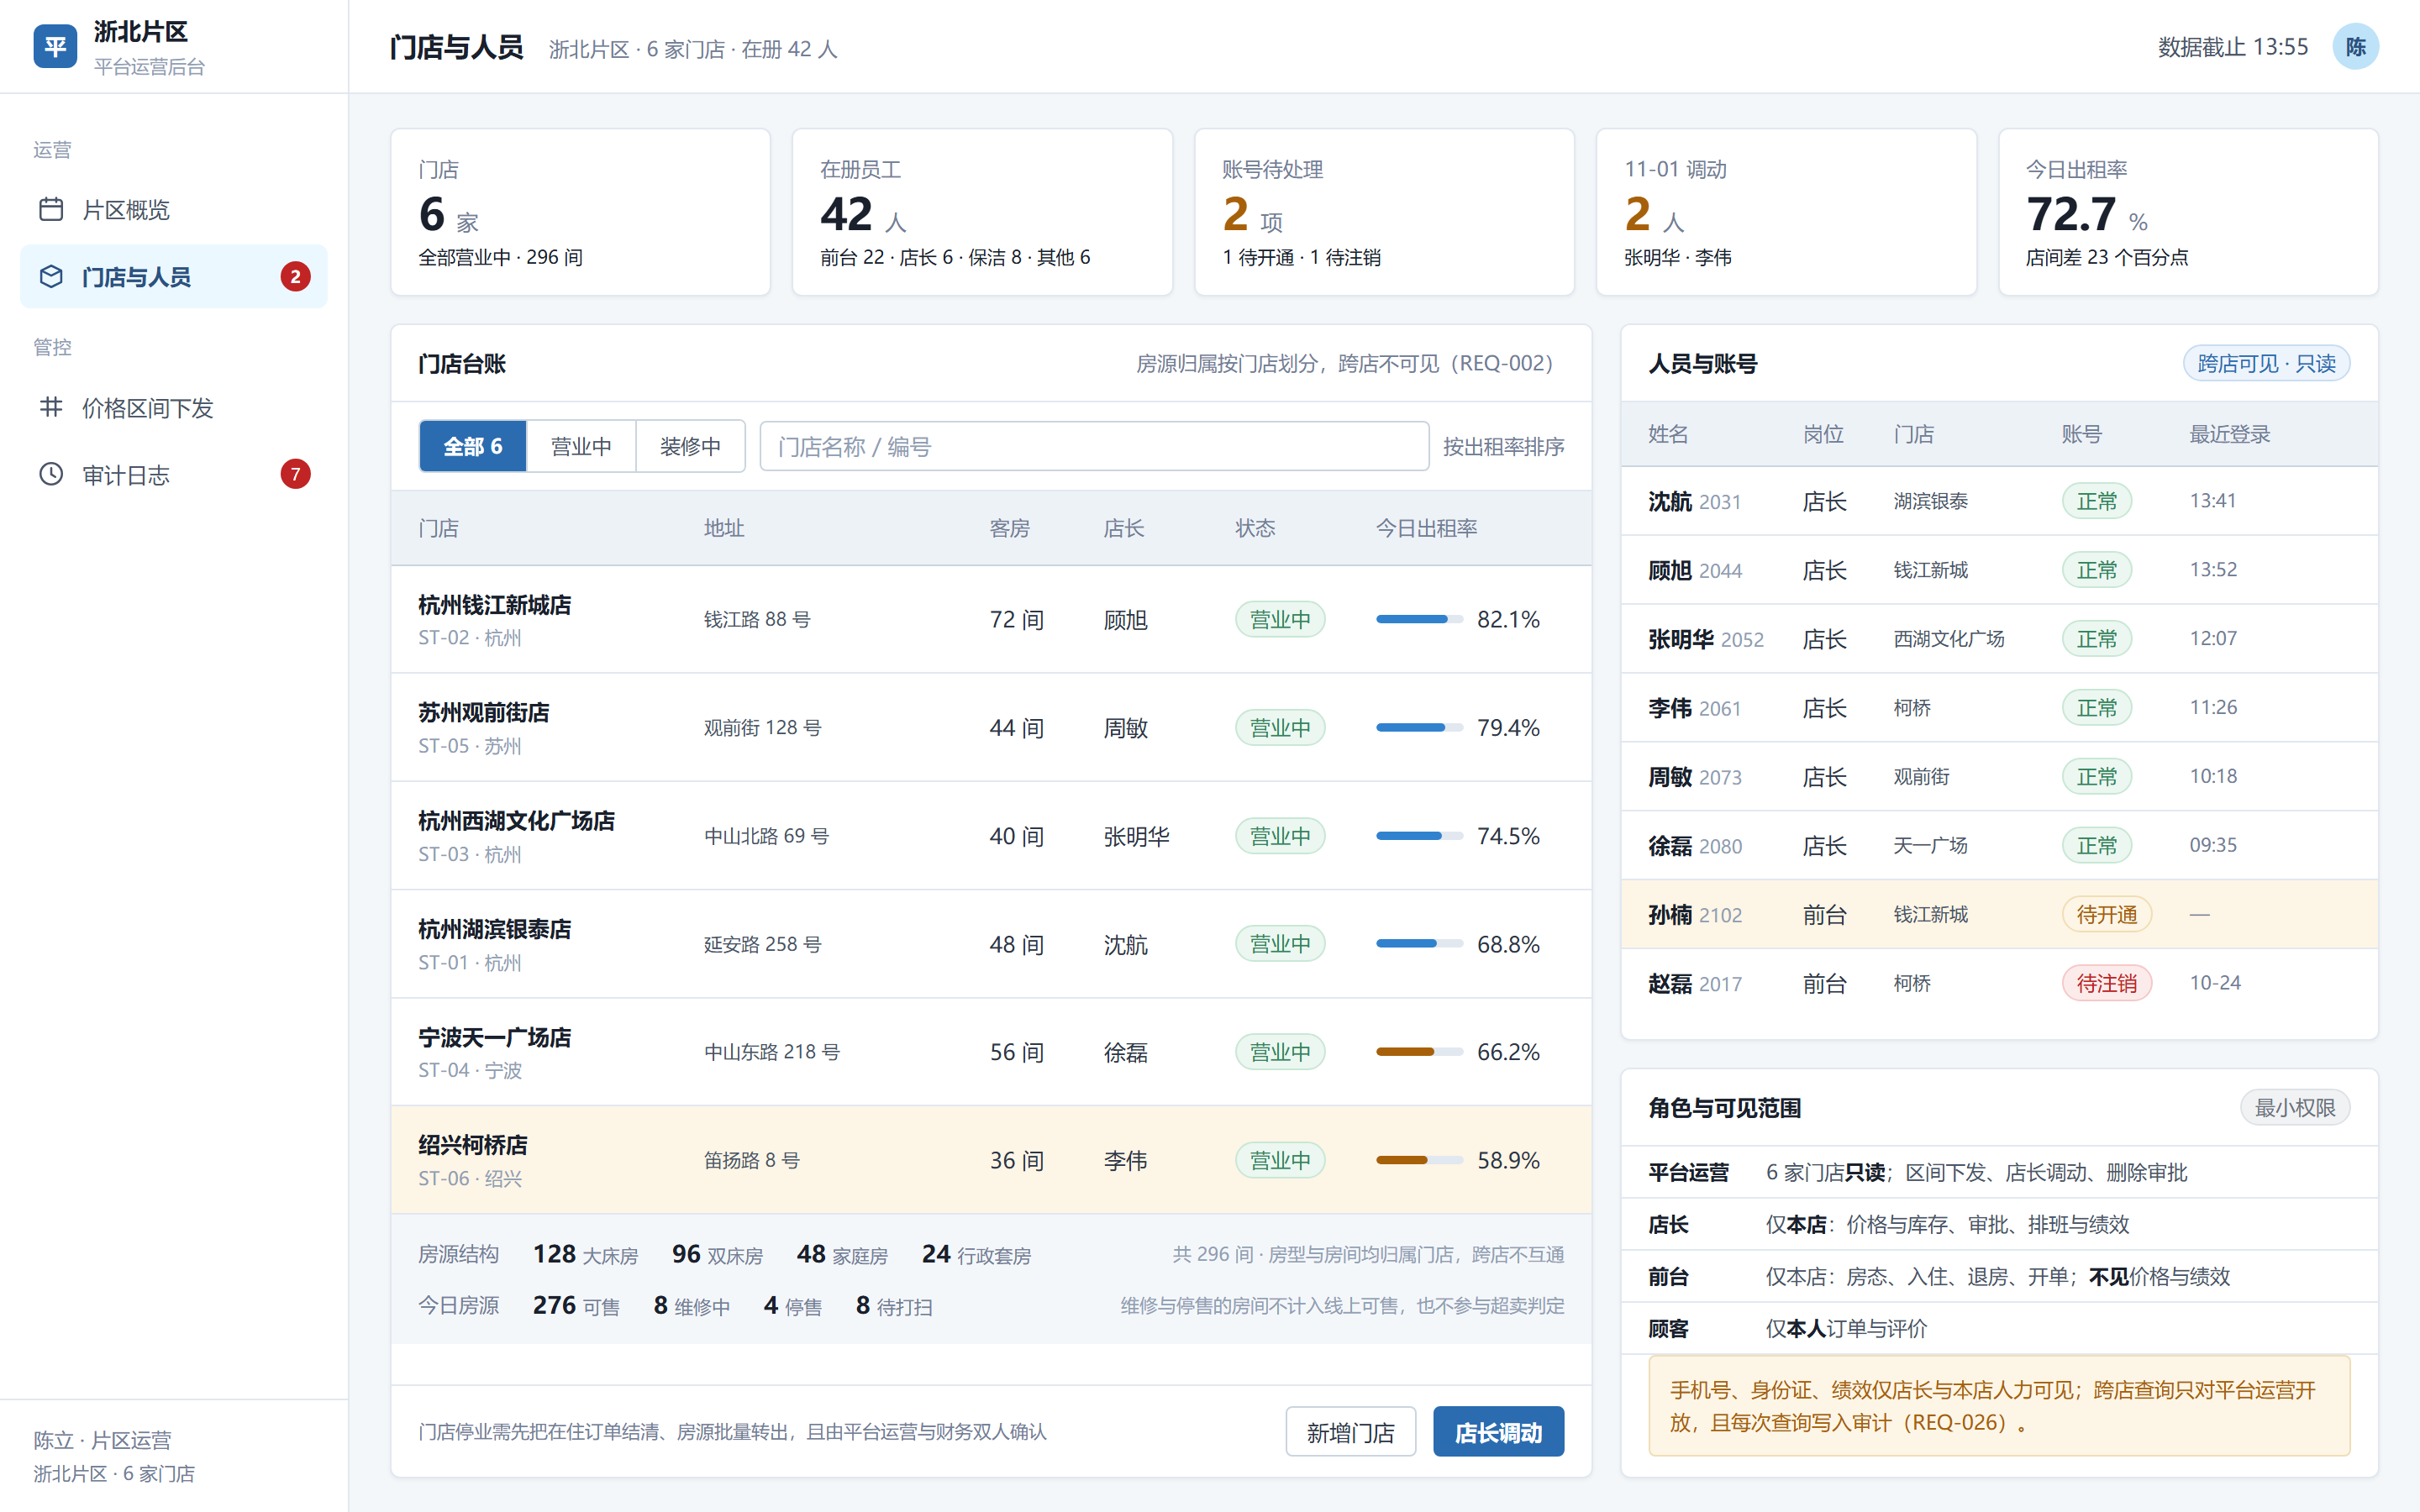
\includegraphics[width=\textwidth]{../UI界面/19_store_staff.png}
  \caption{门店与人员}
\end{subfigure}
\caption{平台端：审计与组织（18--19）}
\label{fig:ui_p2}
\end{figure}

\textbf{18 审计日志与删除审批。} 日志按时间列出操作人、动作、对象及结果，包含被拦截操作和系统定时任务；记录只追加、保留三年。删除审批展示复核进度，要求执行人与申请人不同；跨店查询同样留痕（REQ-014、REQ-026、REQ-030）。

\textbf{19 门店与人员。} 展示六家门店的房量、出租率、负责人及员工账号状态；调动在生效日前标为待生效，离职账号停用但保留历史操作。页面按角色展示可见范围，店长限本店、前台限本店业务、顾客限本人记录（REQ-001、REQ-026）。

\subsection{界面—模块—需求对照}

下表列出 19 屏界面对应的主要模块与需求。

{\tabfont
\begin{xltabular}{\textwidth}{@{}L{0.6cm}L{3.3cm}L{2.4cm}X@{}}
\caption{界面、模块与需求的对应关系}\label{tab:ui_map}\\
\toprule
\# & 界面 & 主要模块 & 落地的需求 \\
\midrule
\endfirsthead
\toprule
\# & 界面 & 主要模块 & 落地的需求 \\
\midrule
\endhead
\midrule
\multicolumn{4}{r}{\zihao{6}续下页}\\
\endfoot
\bottomrule
\endlastfoot
01 & 首页与搜索 & M2、M4 & REQ-002 查询；REQ-019 范围约束 \\
02 & 搜索结果 & M2、M4 & REQ-002；REQ-013 按日期逐晚的余量 \\
03 & 酒店详情与房型 & M2、M3、M4 & REQ-013 可订量取最小；REQ-023 明码标价 \\
04 & 订单确认 & M3、M5 & REQ-020 倒计时；REQ-023 价格快照；REQ-021 取消政策 \\
05 & 支付 & M6、M5 & REQ-020 超时释放；REQ-021 取消截止；REQ-028 一致性 \\
06 & 我的订单 & M5 & REQ-008 六态筛选；REQ-031 改期入口；REQ-003 评价入口 \\
07 & 评价提交 & M8 & REQ-003 仅已退房可评、一单一评 \\
08 & 房态看板 & M7、M2 & REQ-005 六种房态；REQ-022 超时未退；REQ-034 维修与可售 \\
09 & 排房与入住 & M7、M5 & REQ-018 三步入住；REQ-004 入住；REQ-024 排房占房 \\
10 & 退房与打扫 & M7 & REQ-003 退房；REQ-022 逾期；REQ-025 打扫工单 \\
11 & 线下开单 & M4、M5 & REQ-033 上限与线下保留；REQ-032 多晚次 \\
12 & 价格与库存日历 & M3、M4 & REQ-006 店长设价；REQ-033 上限；REQ-013 逐晚库存 \\
13 & 审批中心 & M3、M4、M5、M9 & REQ-014 留痕；REQ-021 取消审批；REQ-025 工单；REQ-034 维修 \\
14 & 排班与评价 & M8 & REQ-026 员工信息范围；REQ-003 评价；REQ-007 绩效汇总 \\
15 & 片区概览与绩效 & M8、M1 & REQ-007 平台管理；REQ-026 可见范围 \\
16 & 价格区间与人员调动 & M3、M1、M9 & REQ-007；REQ-030 删除审批；REQ-009 幂等退款留痕 \\
17 & 消息中心 & M10、M5 & REQ-029 通知失败不回滚；REQ-010 事件订阅 \\
18 & 审计日志与删除审批 & M9 & REQ-030 双人复核与回避；REQ-014 操作留痕；REQ-026 可见范围 \\
19 & 门店与人员 & M1、M2 & REQ-001 账号与权限；REQ-002 门店归属；REQ-026 员工信息范围 \\
\end{xltabular}
}

REQ-035、REQ-036 在实验一尚未确认，因此界面未设计对应流程。性能、可靠性等全局约束不单独设置界面；权限通过各端可见菜单和操作范围体现。

% ==================== 七、AI 辅助设计的使用记录 ====================
\section{AI 辅助设计的使用记录}

\subsection{记录方式与口径}

本章记录本设计中五次实际使用大模型的过程。记录遵守两条自我约束：

\begin{itemize}
  \item \textbf{只记真实发生的事}——AI 给了什么、我判断了什么、最后改成了什么。没有发生过的「人工修改」一律不写，包括那些看起来更漂亮的例子。
  \item \textbf{缺点写具体到错在哪一句}。只写「AI 有幻觉、需人工核对」没有信息量；要写清它倾向了什么、为什么这个倾向在本作业里站不住。
\end{itemize}

五次使用覆盖了本设计的不同环节，其分布本身就是对「AI 能做什么、不能做什么」的答案：

\begin{table}[H]
\centering
\caption{五次使用记录概览}
\tabfont
\begin{tabularx}{\textwidth}{@{}L{1.3cm}L{3.0cm}L{3.4cm}X@{}}
\toprule
编号 & 使用场景 & 产出物 & 暴露的主要缺陷 \\
\midrule
U-01 & 模块划分维度的比较 & 模块划分方案与模块清单 & 对「交付约束」（每模块需有界面）不敏感 \\
U-02 & 下单链路的依赖推导 & 组件图的调用依赖 & 举出的具体例子本身是错的 \\
U-03 & 五处职责与接口分歧 & 职责表、组件图画法 & 在「好看」与「合规」冲突时选好看 \\
U-04 & 19 屏跨屏数据一致性核对 & 修正后的 19 屏界面 & 单屏自洽、跨屏互斥；补屏另起一套事实 \\
U-05 & 报告自身的图表与引用自检 & 修正后的章节与编号 & 引用关系一旦篇幅变长即失效 \\
\bottomrule
\end{tabularx}
\end{table}

\subsection{U-01：模块划分方式的比较与取舍}

\textbf{使用场景。} 作业要求「写明软件的模块划分」，但实验一的 36 条需求是平铺编号的，本身没有模块结构，模块必须重新构造。这一步没有唯一正确答案，需要先知道有哪几种切法。

\textbf{输入与生成结果。} 输入实验一的完整需求清单与实验二的要求，AI 给出三种切法：A 按角色切（顾客 / 前台 / 店长 / 平台）；B 按业务能力切（每模块负责一类业务，多角色共用）；C 按订单生命周期切（搜索 $\rightarrow$ 下单 $\rightarrow$ 支付 $\rightarrow$ 入住 $\rightarrow$ 退房 $\rightarrow$ 售后）。它推荐 B，并给出十个模块草案：账号与权限、门店与房源、定价、库存、预订与订单、支付与退款、房态与工单、评价、审计与数据保留、通知。

\textbf{优缺点分析。} 长处是\textbf{一次给出多个维度并说明各自代价}，比只给一个方案更容易做判断；把 36 条需求批量归类很省时，人工逐条归类容易漏。不足是\textbf{它对作业的交付约束不敏感}：作业要求「为每个功能模块设计 UI 界面」，而「通知」模块没有任何界面——短信与推送发生在业务事件背后，用户看不到它。AI 给的是一个技术上漂亮、在作业里却站不住的划分。此外，模块规模是否失衡需要人自己数一遍条数才看得出来，AI 不主动提醒：评价、通知、支付各只对应 1 条需求，预订与订单对应 8 条。

\textbf{修改优化后的结果。} 采用 B，但做了两处调整：① 通知模块按「无界面」的理由并入预订与订单，模块数从 10 降到 9；② REQ-009（取消与退款）原本整条挂在预订模块，导致「退款执行」归谁不清楚，把退款执行划到支付与退款，取消规则仍留在预订。另确认五条横切约束不挂单个模块：REQ-015 性能、REQ-017 可靠性、REQ-018 易用性、REQ-019 范围、REQ-027 输入校验。

\textbf{一处必须交代的出入。} 以上记录发生在模块划分的阶段，当时的结论是 9 个模块。报告第 2 章与组件图用的是 \textbf{10 个模块}——成稿时通知被重新独立为 M10，理由有三：其一，它在组件图上以「事件订阅者」的身份出现，与调用依赖的形态不同，合并进 M5 会让 M5 同时承担业务与通知两种职责；其二，REQ-029 要求通知失败进入独立失败队列并重试，这个失败语义不能污染订单事务；其三，通知的站内消息在界面上是可查的（消息记录与重试状态），因此「无界面」这个最初的排除理由在重新审视时不成立。需要说明的是，写这段话时第三条还只是一个判断——直到第 6 章补出 17 屏消息中心，它才真正落到界面上；界面反过来也证伪了最初的理由。这不是事后补的理由，而是这次比对暴露出的结论：\textbf{「有没有界面」这条判据本身是模糊的}，它取决于界面定义到哪一层，用它做排除条件时要格外小心。

\subsection{U-02：下单链路上模块交互的推导}

\textbf{使用场景。} 模块划分完成后，需要说清模块之间怎么交互，这是组件图与时序图的依据。计划用「走一遍具体业务流程」的办法推导依赖关系，而不是直接罗列「A 依赖 B」。

\textbf{生成结果。} 按步骤走完「顾客提交订单 $\rightarrow$ 订单变待支付、库存被占住」这条链路，得出主控为预订与订单，依赖账号与权限、定价、库存、审计，并说明门店与房源、支付与退款不参与的原因；据此提出三根单向箭头。

\textbf{优缺点分析。} 长处是\textbf{按业务流程逐步推导，比直接罗列更易发现遗漏}，并且能主动指出「哪些模块不该参与」——这一步用「不参与」的方式把边界划清楚了。不足很严重：\textbf{它给出的具体例子本身是错的}。它举「M4 库存释放后调 M5 会成环」作为需要避免的例子，但库存释放由订单取消触发，本来就是 M5 调 M4，箭头方向没变，不存在环。真正成环的位置是 M5 与 M6 之间（下单创建支付单是 M5$\rightarrow$M6，支付回调改订单状态是 M6$\rightarrow$M5）。\textbf{而且它不会自己发现这个错误}，需要人拿需求原文逐条去对。

\textbf{修改优化后的结果。} 下单链路确定为 M5 主控、三根单向依赖（M5$\rightarrow$M3、M5$\rightarrow$M4、M5$\rightarrow$M1）；M5 与 M6 之间的环用\textbf{事件}拆开——M6 支付成功后发布「支付已成功」事件，M5 订阅后自行推进订单状态，M6 不调用 M5。同时确定两处细节：支付单在用户点「去支付」时才创建，不在下单时创建，使支付网关故障不波及下单；库存与订单在同一事务内\textbf{先扣库存再建订单}，因为扣库存是链路上唯一会失败的关键动作，放在最前可以让失败的请求尽早退出。这两条后来成了第 3 章的决策四与决策一。

\subsection{U-03：模块职责与接口的五处分歧判断}

\textbf{使用场景。} 按九个模块起草职责与接口表时，有五处存在两种都说得通的写法，需要定一种并落到表里：① 横切依赖（M1、M9 被所有模块依赖）在组件图上怎么画；② 排房归门店与房源还是房态与工单；③ 22:00 未到店判定归预订模块还是房态模块；④ 线上可售上限由店长直接设定还是由公式算出；⑤ 取消后释放库存用同步调用还是事件。

\textbf{生成结果。} 针对五处各给出甲乙两案，并附上自己的倾向。

\textbf{优缺点分析。} 长处是\textbf{先把「存在两种写法」这件事摆出来}，这比只给一个答案有用得多——有几处（例如排房到底归谁）在提问之前完全没想到要选；附上倾向也便于快速判断。不足是\textbf{它的倾向未必对，而且错得很有代表性}：第 ① 处它倾向「不画箭头，只在图下注一句『所有模块依赖 M1 与 M9』」，理由是画了会糊掉，却没意识到那样这两个模块根本不会出现在组件图上，而作业明确要求写明模块划分，缺了这两块等于交了一张残缺的图。\textbf{它优化的是图的观感，不是作业的达标线}。

\textbf{修改优化后的结果。} 逐条定为：

\begin{enumerate}[leftmargin=3.2em]
  \item \textbf{改为与 AI 相反}：把 M1、M9 画成底部一条「公共支撑」带，各业务模块汇一根总箭头过去。同时在正文里明写这个折中本身违反「画全」原则及原因，不让它悄悄消失。
  \item 采纳：M2 只管房间档案，占房与释放房号是 M7 的事。
  \item 采纳：M5 的定时任务自己判定 22:00 未到店，M7 只回答「这单今天入住没有」——改的是订单状态，就该由订单模块主导。
  \item 采纳：可售上限以公式（房间总数 $-$ 维修 $-$ 线下保留）为天花板，店长可在此基础上\textbf{手动下调，但不得高于公式值}。这一条同时满足 REQ-006 的「可设置」与 REQ-033 的「按公式重算」，也是第 4 章那条公式的由来。
  \item 采纳：M5 \textbf{同步调用} M4 释放库存，不经过事件。释放失败会让库存长期被占、直接少卖房，这种事必须当场知道。
\end{enumerate}

\subsection{U-04：19 屏跨屏数据一致性核对}

\textbf{使用场景。} 19 屏界面按屏逐个生成时，每一屏单独看都自洽；但界面之间共享同一批数字（房量、出租率、价格、营收），一旦某一屏单独改动，就会出现「两套事实」。因此在 19 屏齐备后，做了一轮逐屏对账。

\textbf{生成结果与发现的问题。} 核对的方法是：先固定 1.5 节的六条数据基准，再把每一屏上出现的数字抽出来与基准比对。发现的问题可分为三类：

\begin{itemize}
  \item \textbf{跨屏不一致}：片区概览的营收环比写作 $+4.8\%$，但片区合计营收 ¥113,721 与前一日推算值对应的是 $+2.0\%$；门店排班页的「今日当班」人数与下方排班表实际当班行数对不上；顾客端各屏的门店评分写作 4.8，而后台门店档案与详情页统一是 4.6。
  \item \textbf{单屏金额算错}：订单列表里「一居室公寓 2 晚」的已付金额写作 ¥588，应为 ¥588 $\times$ 2 = ¥1,176；酒店详情页的「剩 3 间」与两晚库存取最小值 $\min(4,1)=1$ 矛盾，应为「剩 1 间」。
  \item \textbf{规则被界面悄悄改写}：支付页的取消政策原文暗示「18:00 之后可自助取消」，与 REQ-021（18:00 后转前台代提交 + 店长审批）直接冲突；平台端的退款案例时间落在 18:00 之后却走的是自助链路。这类错误最危险——\textbf{数字错了只是难看，规则错了会让人以为系统支持一个它并不支持的操作}。
  \item \textbf{补屏时另起一套事实}（补齐 17--19 屏时才暴露）：门店与人员屏的门店清单是另编的六家（富阳、临平、武林门等），房量与出租率与 15 屏完全不同，页头的「今日出租率 78.6\%」也不等于任一组按房量加权的值。原因是\textbf{后生成的屏没有去读已有屏的数字}，它只从「六家门店」这个描述出发重新编了一遍。同一批里还有身份冲突：同一个人在一部分屏是「湖滨银泰店长」、在平台三屏却是「片区运营」，审计屏甚至出现「操作人 $\times\times$ · 批准人 $\times\times$」的同人自批——正好撞在 REQ-030 的回避规则上。
\end{itemize}

\textbf{优缺点分析。} 长处是\textbf{生成速度与一致的单屏质量}：19 屏在结构、间距、状态色上高度一致，这是逐屏手画很难达到的。不足是\textbf{它没有跨屏的全局状态}——每次只在一个上下文中生成一屏，看不见其他屏上的数字；而设计里最需要一致的东西恰恰是跨屏的。此外它对业务规则的理解是「读到的这句话」，而不是「这条规则在所有界面上应该怎么体现」，所以会在不同屏上给出互相矛盾的倾向。

\textbf{修改优化后的结果。} 建立「单一事实源」：48 间房的六种房态相加必须等于 48、48 间 $\times$ 价格 $\times$ 出租率必须能解释当日营收、片区 6 店按房量加权的出租率必须等于 72.7\%。三道校验写进报告 1.5 节，之后任何一屏改数字都要过这三道；上列问题逐条修正并重新导出。

第三类问题（补屏另起一套事实）的修法与数字不同，它要求\textbf{先指定一屏为权威副本}：门店清单以 15 屏为准，19 屏逐行照抄同一组门店名、房量与出租率，房源结构的两条汇总也按 296 间重新配平，使两行各自的和都等于门店房量之和；身份冲突则改成一个人只有一个角色——片区运营另有其人，店长名只出现在本店语境里，审计屏的自批条目改写为「区间内无需审批」，删除申请的申请人与复核人拆成两个不同的人。这类修改必须\textbf{改到源文件再重新导出}，不能在导出图上修图，否则下一轮重导又回到错误状态。

\subsection{U-05：报告自身的图表与引用自检}

\textbf{使用场景。} 报告正文较长，图、表、决策条目、章节之间大量互相引用。写完后需要确认「文中提到的编号确实存在」。

\textbf{生成结果与发现的问题。} 逐章交叉检查引用，发现两处：

\begin{itemize}
  \item 第 2 章追溯矩阵把 REQ-015 引向「3.5 决策五」、REQ-016 引向「决策六」，但当时的决策表只有六行，且第五条讲的是状态机、第六条讲的是价格快照——\textbf{编号对得上，内容对不上}。
  \item 第 1 章与第 5 章开头都写「画了 14 张 UML 图」，实际目录里是 16 张；类图说明写「23 个类」，实际数是 24 个。
\end{itemize}

\textbf{优缺点分析。} 长处是\textbf{一致性检查适合交给模型}：这类问题是纯机械的比对，不涉及业务判断，AI 做得又快又全，比人工翻页可靠。不足是\textbf{它会在改一处时引入新的一处}——决策表扩成八条之后，如果没有重新对一遍所有引用，就会出现「新加的第七条没人引用、旧的第五条被错指」的二次问题。\textbf{一致性不是一次检查，而是每次改动后都要重跑的东西}。

\textbf{修改优化后的结果。} 决策表由六条扩为八条（新增决策七「查询走缓存、写落主库」与决策八「鉴权在网关一次做完」），并把第 2 章的引用改为决策七 / 决策八 / 决策三；图的张数与类的数量按实际改。这里有一个值得记下的教训：\textbf{写「第 N 章」「决策 N」这类相对编号，比写「3.5 节决策三」更容易在扩写后失效}，因此定稿时应统一按「章-节-序号」的绝对位置引用。

\subsection{大模型如何辅助软件设计}

把五次记录横过来看，AI 在本设计中的实际作用是清楚的：

\begin{table}[H]
\centering
\caption{AI 在设计各环节的实际作用与人的介入点}
\tabfont
\begin{tabularx}{\textwidth}{@{}L{2.9cm}L{4.8cm}X@{}}
\toprule
设计环节 & AI 做了什么事 & 人必须做的事 \\
\midrule
需求理解 & 把 36 条需求批量归类到模块 & 判断分类是否违背交付约束；发现规模失衡 \\
模块划分 & 给出多种划分维度与各自代价 & 按作业要求排除「无界面」的模块；定最终切法 \\
依赖推导 & 按业务流程逐步推依赖 & 拿需求原文核对每一个具体例子 \\
图与界面生成 & 生成 PlantUML 与 19 屏界面，风格统一 & 检查规则是否被界面悄悄改写；跨屏数字对账 \\
文本与编号 & 起草正文、维护图表编号与引用 & 判断编号背后指的到底是不是那个意思 \\
\bottomrule
\end{tabularx}
\end{table}

一句话概括：\textbf{AI 擅长的是「把已有约束铺开」，不擅长的是「判断哪条约束在这件事上更硬」。} 它能快速生成十个候选、九条依赖、十九屏界面，但它不知道「每个模块要有界面」是这个作业的达标线、「18:00 后不能自助取消」是业务红线——它只知道这些字出现在输入里。

\subsubsection{能否设计一套工作流，让人只做检查校对}

作业的结尾问题值得认真回答。结论是：\textbf{能做到「人只做检查校对」，但校对这一步不能简化成「看一眼」。}

一条可行的工作流分五步，前四步可以自动化，第五步不行：

\begin{enumerate}[leftmargin=3.2em]
  \item \textbf{结构化输入}。把需求写成带编号的条目（本设计的 REQ-001～036），把数据基准写成一张表（本设计的 1.5 节），把交付约束单独列成清单（图的类别与下限、每模块需有界面、提交物结构）。这一步是整条流水线的价值来源：\textbf{能被机器校验的东西，前提是它先被写成了可校验的形状}。
  \item \textbf{分单元生成}。按图、按屏、按章分别生成，每个单元附一句「本单元落了哪几条 REQ」。
  \item \textbf{机器校验}。三类自动检查：PlantUML 语法编译通过；REQ 覆盖矩阵与需求清单做差集，找出没被任何单元引用的需求；跨单元数值比对，把同一实体在不同单元上的数字列出来看是否相等。
  \item \textbf{差异回写}。把第三步的结果原样喂回生成环节，让模型只改被指出的位置，而不是整段重写——避免 U-05 里那类「改一处引入另一处」。
  \item \textbf{人工校对}。人只做三件机器做不了的事：\textbf{判断约束的优先级}（作业要求与图面观感冲突时，哪一个是达标线——U-03 的第 ① 处）；\textbf{判断「算得对」之外是否「说得对」}（U-04 里「18:00 后自助取消」数字全对但规则错了，这类机器查不出来）；\textbf{判断需求本身是否成立}（REQ-035、REQ-036 至今标为待确认，任何生成物都不该替实验一把它确认掉）。
\end{enumerate}

因此答案是：\textbf{可以让一个人一天之内完成原本一周的设计工作量，但那个人的角色从「画图的人」变成了「定判据的人」}。他的产出不再是一张图，而是那三条机器能读的输入——需求编号、数据基准、交付约束清单。这三样东西写不清，整条流水线产出的就是一堆漂亮而互相矛盾的东西；写清了，检查校对才真的只是检查校对。

反过来说，本设计里 AI 出的每一个错，追根到底都不是「模型能力不够」，而是\textbf{判据没有提前写下来}：模块划分时「有没有界面」是个模糊判据，于是它把通知塞进了订单模块；数据基准是逐屏才浮现的，于是出现了 ¥588 与 ¥1,176；决策编号是相对的，于是扩写后引用全错。\textbf{把判据前置，是这个工作流唯一真正的难点，也是最不能被 AI 代劳的部分。}

% ==================== 八、实验总结与不足 ====================
\section{实验总结与不足}

\subsection{设计产物概览}

本报告各章给出的设计产物如下，便于按图查阅：

\begin{table}[H]
\centering
\caption{各章的设计产物}
\tabfont
\begin{tabularx}{\textwidth}{@{}L{2.2cm}L{4.2cm}L{2.6cm}X@{}}
\toprule
章节 & 设计产物 & 规模 & 内容 \\
\midrule
第 2 章 & 功能划分与需求追溯 & 10 个模块、36 条需求 & 需求逐条落模块，跨模块与不覆盖的单独标注 \\
第 3 章 & 架构设计与模块交互 & 包图 / 组件图 / 部署图 & 模块依赖、交互链路与八条设计决策的代价 \\
第 4 章 & 数据库设计 & 22 张表 & 字段、索引、唯一约束与库存条件更新 \\
第 5 章 & UML 建模 & 16 张图 & 结构 4 张、行为 8 张、交互 4 张，均为 PlantUML 源码加导出图 \\
第 6 章 & 界面设计与功能描述 & 19 屏 & 四端各屏的元素、状态及对应需求 \\
第 7 章 & AI 协作过程记录 & 设计阶段 7 组，另有报告改稿 & 事前讨论、生成结果、优缺点与本人校改 \\
第 7 章末 & 人机分工流程 & 一条五步流程 & 从确定内容到核对结果均保留人的判断 \\
\bottomrule
\end{tabularx}
\end{table}

\subsection{主要设计结果}

本次完成的主要设计内容为：

\textbf{库存。} 日库存按房型和晚次记录，同房型请求先赋序再处理；下单采用条件更新与事务回滚，避免并发超卖（REQ-011）。并发抢房流程见第 5.6 节。

\textbf{状态。} 分别绘制订单与房间状态图，列出订单转换条件，非法转换统一拒绝（REQ-005、REQ-008）。

\textbf{界面。} 绘制 19 屏并建立界面与需求的对应表。09 屏展示三步入住；11 屏展示线下保留额度不足时拒绝开单，并提示引导客人线上预订或由店长先调整额度（REQ-018、REQ-033）。

这次设计中，我对「预订成功」和「分配房号」的区别理解得更清楚了。下单时按房型和日期占库存，入住前才给订单安排具体房间；因此类图中需要单独的占房记录，前台界面也要能查看哪些房间在相应日期可分配。把这两个步骤拆开后，库存模型、类图和入住流程之间的关系才说得通。

报告和界面初稿由 AI 辅助生成，我负责对照实验一需求核对设计内容。19 屏界面完成后，曾出现跨屏余量、取消文案与业务规则不一致的问题；我依据统一示例数据和需求编号提出修改意见，再检查改后的图稿。这个过程让我发现，界面和 UML 图除了展示方案，也能用来检查前面讨论的规则有没有真正落到每个操作上。AI 的具体使用与修改记录见第 7 章。

\subsection{后续细化}

\textbf{接口细节。} 本次确定了模块职责和调用方向，具体方法参数、返回值及错误码可在实现时补齐。

\textbf{界面状态。} 19 屏已覆盖主要操作；支付失败、搜索无结果等提示还可在现有界面上补充。

% ==================== 附录 ====================
\newpage
\appendix
\ctexset{
  section = {
    name   = {附录},
    number = \Alph{section},
    format = \heiti\zihao{3}\raggedright,
  },
}

\section{需求—模块—图—界面 追溯矩阵}

本附录把实验一的 36 条需求一次性映射到模块、UML 图与界面，用于核对「有没有哪条需求在设计里落了空」。「主要图」列取自第 5 章的 UML 图清单（表~\ref{tab:uml_list}）；界面号按第 6 章的 01--16 屏；「—」表示该需求不在界面层体现（属于后端能力或范围约束）。

{\tabfont
\begin{xltabular}{\textwidth}{@{}L{1.75cm}L{2.75cm}L{2.65cm}L{3.75cm}X@{}}
\caption{需求追溯矩阵}\label{tab:app_trace}\\
\toprule
需求 & 名称 & 模块 & 主要图 & 界面 \\
\midrule
\endfirsthead
\toprule
需求 & 名称 & 模块 & 主要图 & 界面 \\
\midrule
\endhead
\midrule
\multicolumn{5}{r}{\zihao{6}续下页}\\
\endfoot
\bottomrule
\endlastfoot
REQ-001 & 角色定义与最小权限 & M1 & 用例图 $\times$4、包图 & — \\
REQ-002 & 顾客查询与预订 & M2/M4/M5 & 类图、活动图 1 & 01, 02, 03, 04 \\
REQ-003 & 退房与评价提交 & M7/M8 & 状态图·订单、用例图·顾客 & 06, 07, 10 \\
REQ-004 & 前台办理入住 & M7 & 用例图·前台、状态图·房间 & 09 \\
REQ-005 & 房间状态机 & M7 & 状态图·房间 & 08, 09, 10 \\
REQ-006 & 店长门店管理 & M2/M3/M4/M7 & 用例图·店长、类图 & 12, 14 \\
REQ-007 & 平台地区负责人管理 & M1/M3/M8 & 用例图·平台 & 15, 16 \\
REQ-008 & 订单状态机 & M5 & 状态图·订单 & 06 \\
REQ-009 & 取消与退款 & M5/M6 & 类图、时序图·超时释放 & 05, 06, 16 \\
REQ-010 & 重复提交防护 & M5 & 活动图 1、类图 & 04 \\
REQ-011 & 并发抢房 & M4 & 时序图·并发抢房、活动图 1 & 03 \\
REQ-012 & 改价与下单隔离 & M3 & 时序图·改价互斥 & 12, 13 \\
REQ-013 & 库存与可售上限 & M4 & 类图、组件图 & 02, 03, 12 \\
REQ-014 & 操作日志 & M9 & 组件图 & 13, 16 \\
REQ-015 & 性能 & 横切 & 部署图 & — \\
REQ-016 & 安全 & 横切 & 包图、部署图 & — \\
REQ-017 & 可靠性与数据一致 & 横切 & 部署图 & — \\
REQ-018 & 易用性 & 横切 & 用例图·前台 & 09 \\
REQ-019 & 范围约束 & 约束 & — & — \\
REQ-020 & 支付超时释放 & M5/M6 & 状态图·订单、时序图·超时释放 & 04, 05 \\
REQ-021 & 取消截止与前台代取消 & M5 & 状态图·订单、用例图·顾客 & 05, 06 \\
REQ-022 & 未到店标记与迟入住 & M5/M7 & 状态图·订单 & 08, 10 \\
REQ-023 & 价格快照与定价依据 & M3/M5 & 类图（明细单价快照） & 03, 04 \\
REQ-024 & 房号分配 & M7 & 类图（占房记录）、用例图·前台 & 09 \\
REQ-025 & 房态变更工单 & M7 & 类图（工单）、用例图·前台 & 10, 13 \\
REQ-026 & 员工信息可见范围 & M1 & 用例图 $\times$4 & 14, 15 \\
REQ-027 & 输入校验与错误提示 & 横切 & 活动图 1 & 04, 11 \\
REQ-028 & 支付与订单一致性 & M6/M5 & 时序图·支付回调、时序图·超时释放 & 16 \\
REQ-029 & 通知失败处理 & M10 & 组件图 & — \\
REQ-030 & 数据保留与删除审批 & M9 & 用例图·平台 & 16 \\
REQ-031 & 订单变更 & M3/M4/M5 & 用例图·顾客 & 06 \\
REQ-032 & 多房型多晚次组合 & M4/M5 & 类图（明细唯一约束） & 11 \\
REQ-033 & 线上可售上限与线下保留 & M2/M4 & 组件图、类图 & 11, 12, 13 \\
REQ-034 & 维修中与可售上限联动 & M2/M4/M7 & 状态图·房间、组件图 & 08, 12, 13 \\
REQ-035 & 订单排房时限 & —— & —— & 待确认，不覆盖 \\
REQ-036 & 账号注册与登录 & —— & —— & 待确认，不覆盖 \\
\end{xltabular}
}

从这张表可以读出三件事：第一，36 条需求中 34 条有设计落点，2 条因实验一未确认而明确不覆盖；第二，被引用最多的图是类图与组件图，说明「数据形状」与「模块边界」是本设计的两根主线；第三，有四条需求（REQ-015、016、017、019）在图与界面上都没有单独落点，它们是被全系统共享的非功能约束——这类需求不应硬塞给某个模块，写清「为什么不单独落点」比强行分配更有说服力。

\needspace{9cm}
\section{提交物清单}

提交包解开后是一层根目录加两个子目录。\texttt{UML/} 下每个 \texttt{.png} 都配有一份同名的 \texttt{.puml}（16 组、32 个文件），下表只列 \texttt{.png}。

{\zihao{5}\ttfamily\raggedright
\noindent 实验2\_241220031\_曹继贤/\par
\noindent\hspace*{2em}实验报告.pdf\par
\noindent\hspace*{2em}UML/\par
\noindent\hspace*{4em}UML类图.png\qquad UML包图.png\par
\noindent\hspace*{4em}UML组件图.png\qquad UML部署图.png\par
\noindent\hspace*{4em}UML用例图\_顾客端.png\qquad UML用例图\_前台端.png\par
\noindent\hspace*{4em}UML用例图\_店长端.png\qquad UML用例图\_平台端.png\par
\noindent\hspace*{4em}UML状态图\_订单.png\qquad UML状态图\_房间.png\par
\noindent\hspace*{4em}UML活动图\_下单与锁库存.png\qquad UML活动图\_支付回调与订单生效.png\par
\noindent\hspace*{4em}UML时序图\_并发抢房.png\qquad UML时序图\_改价互斥.png\par
\noindent\hspace*{4em}UML时序图\_支付回调.png\qquad UML时序图\_超时释放与对账.png\par
\noindent\hspace*{2em}UI界面/\par
\noindent\hspace*{4em}01\_home\_search.png\qquad 02\_search\_result.png\par
\noindent\hspace*{4em}03\_hotel\_detail.png\qquad 04\_order\_confirm.png\par
\noindent\hspace*{4em}05\_payment.png\qquad 06\_my\_orders.png\par
\noindent\hspace*{4em}07\_review\_submit.png\qquad 08\_room\_board.png\par
\noindent\hspace*{4em}09\_checkin.png\qquad 10\_housekeeping.png\par
\noindent\hspace*{4em}11\_walkin\_order.png\qquad 12\_price\_calendar.png\par
\noindent\hspace*{4em}13\_approval\_center.png\qquad 14\_roster\_review.png\par
\noindent\hspace*{4em}15\_region\_overview.png\qquad 16\_price\_range\_staffing.png\par
}

\section{图的绘制方式}

全部 16 张 UML 图由 PlantUML 绘制，源文件（\texttt{.puml}）与导出图（\texttt{.png}）同名放在 \texttt{UML/} 下，可用以下命令重新生成：

\begin{quote}
\zihao{5}\ttfamily
java -jar plantuml.jar -charset UTF-8 -tpng UML/*.puml
\end{quote}

统一的绘图约定：白底、深灰线、单一强调色；中文字体统一为 Microsoft YaHei；结构图与行为图宽度按内容自适应，时序图与活动图固定较窄的画幅以便插入正文。16 屏界面用 HTML 与 CSS 编写后按 2 倍像素密度导出 PNG（顾客端 780 $\times$ 1688，后台 2880 $\times$ 1800），因此插入报告后文字仍可辨认。


\end{document}
